
%% Formato para la presentaci\'on de  proyectos de grado. 
%% Maestría en Ingeniería de Software
%% Pontificia Universidad Javeriana
%% Elaborado por Angela Villota y Luisa Rincón
%% Inspirado en Formato elaborado para carrera de Ing de Sistemas
%% V 1.0 Abril - 2022

\documentclass[11pt]{article}
\usepackage[utf8]{inputenc}
\usepackage{geometry}
\geometry{letterpaper}
\usepackage[spanish,es-tabla]{babel}
\usepackage{cite}
\usepackage{titling}
\usepackage{setspace}
\usepackage{graphicx}
\graphicspath{{img/}} %ruta de la carpeta en donde estaràn las imágenes
\usepackage{blindtext}
% \usepackage{url}
\usepackage{hyperref}
\usepackage{natbib} %% para citaciones
\usepackage[format=hang,font=small,labelfont=bf]{caption}

% *** ALIGNMENT PACKAGES ***
%
\usepackage{array}
\usepackage{booktabs}
\usepackage{pdflscape}
\usepackage{multirow}
\usepackage{float}
\usepackage{longtable}
\usepackage{dblfloatfix}
\usepackage{subfig}
\usepackage{todonotes}
\usepackage{ulem}
\usepackage{xcolor,colortbl}
\usepackage{subcaption}

\onehalfspacing
\setcounter{secnumdepth}{5}
\setcounter{tocdepth}{2}

\usepackage{xcolor}
\definecolor{light-gray}{gray}{0.95}
\newcommand{\code}[1]{\colorbox{light-gray}{\texttt{#1}}}

\renewcommand\maketitlehooka{\null\mbox{}\vfill}
\renewcommand\maketitlehookd{\vfill\null}

\begin{document}
%crear titulo
%\maketitle

%%%%%%%%%%%%%%%%%
% Portada del Anteproyecto
%%%%%%%%%%%%%%%%%
\begin{center}
\thispagestyle{empty}
\vspace*{0cm}
\begin{center}
    
\includegraphics[width=8cm]{pujlogo}~\\[1.75cm]
\end{center}
\textbf{\fontsize{11}{12}\selectfont
Metodología MLOps para la entrega continúa de un modelo de Machine Learning para el reconocimiento y control de las plagas Stenoma catenifer y heilipus lauri en el cultivo de aguacate Hass}\\[1.75cm]
\normalsize\textbf{Juan Felipe Rodriguez Torres}\\[1.5cm]
\small Proyecto presentado como requisito para optar al
t\'{\i}tulo de:\\
\textbf{Magister en Ingenier\'{\i}a de Software}\\[1.5cm]
Director:\\
Ph.D. David Arango Londoño\\[1.6cm]

Pontificia Universidad Javeriana Cali\\
Facultad de Ingeniería\\
Departamento de Electrónica y Ciencias de la Computación\\
Cali, Colombia\\
\today\\
\end{center}

\newpage
%%%%%%%%%%%%%%%%%
% Presentacion Anteproyecto
%%%%%%%%%%%%%%%%%
%%%%%%%%%%%%%%%%%
% Presentacion Anteproyecto
%%%%%%%%%%%%%%%%%
\thispagestyle{empty}
Santiago de Cali, \today

\newcommand{\underlinetext}[2][1pt]{{%
  \renewcommand{\ULdepth}{#1}%
  \uline{#2}%
}}

\begin{flushleft}
Ingeniero: \\
Juan Carlos Martínez Arias \\
Director Posgrados de Ingeniería \\
Facultad de Ingeniería y Ciencias \\
Pontificia Universidad Javeriana - Cali \\
\end{flushleft}


Con el fin de cumplir con los requisitos exigidos por la Universidad para llevar a cabo el Trabajo de Grado y posteriormente optar por el título de Magíster en Ingeniería, nos permitimos presentar a su consideración el anteproyecto de Trabajo de Grado denominado "\textit{Metodología MLOps para la entrega continúa de un modelo de Machine Learning para el reconocimiento y control de las plagas Stenoma catenifer y heilipus lauri en el cultivo de aguacate Hass}", el cual será realizado por el estudiante \textit{Juan Felipe Rodriguez Torres} con código \textit{3070801526} perteneciente al énfasis en Ingeniería de Software, bajo la dirección del profesor \textit{David Arango Londoño}.

El suscrito director del Trabajo de Grado autoriza para que se proceda a hacer la evaluación de este Anteproyecto ante el Tribunal que para el efecto se designe, toda vez que ha revisado cuidadosamente el documento y avala que ya se encuentra listo para ser presentado oficialmente.

\vspace{1cm}

\begin{table}[h]
\begin{tabular}{@{}p{0.5\textwidth} p{0.5\textwidth}@{}}
\textit{Firma Estudiante} \hrulefill & \textit{Firma Director} \hrulefill \\
\textit{Nombre Estudiante} \underlinetext[1pt]{Juan Felipe Rodriguez Torres} & \textit{Nombre Director} \underline{David Arango Londoño} \\
C.C. \underline{1130668332} \textit{de} \underline{Cali} & C.C. \underline{1130586950} \textit{de} \underline{Cali} \\
\end{tabular}
\end{table}

\vspace{1cm}

Documentación anexa:

\begin{itemize}
  \item Una copia del Anteproyecto del Trabajo de Grado.
  \item Ficha Resumen Anteproyecto del Trabajo de Grado.
\end{itemize}

\newpage
%%%%%%%%%%%%%%%%%
% Ficha resumen
%%%%%%%%%%%%%%%%%
\thispagestyle{empty}
\begin{center}
    \Large{Ficha Resumen \\ Trabajo de Grado de Maestría}
\end{center}

\textbf{Título: Metodología MLOps para la entrega continúa de un modelo de Machine Learning para el reconocimiento y control de las plagas \textit{Stenoma catenifer} y \textit{heilipus lauri} en el cultivo de aguacate Hass.}
\begin{enumerate}
    \item Tipo de proyecto: Aplicado
    \item Área de trabajo: Ingeniería de Software
    \item Estudiante: Juan Felipe Rodriguez
    \item Correo electrónico: jfrodriguezt@javerianacali.edu.co
    \item Dirección y teléfono: Carrera 112 48 - 92 Apto 701 Torre 5, 3058176473
    \item Director: Ph. D. David Arango
    \item Correo electrónico del director: david.arango@javerianacali.edu.co
    \item Palabras clave(al menos 5): Big Data, Machine Learning, MLOps, Cultivo de aguacate, Plagas \textit{Stenoma catenifer} y \textit{heilipus lauri}.
    \item Fecha de inicio: 15/Septiembre/2023
    \item Resumen: La creciente aplicación de avances tecnológicos en diversos ámbitos de la vida ha llevado a la adopción de tecnologías innovadoras en la agricultura para mejorar la productividad y la eficiencia. Dentro de estas tecnologías, la metodología MLOps se destaca por su capacidad para mantener la operación de los modelos de aprendizaje automático y su despliegue, mientras se mejora y reentrenan los modelos, en donde se optimiza la toma de decisiones y el aumento de la precisión de los resultados.
\newpage
\thispagestyle{empty}

    La investigación se centra en el cultivo del aguacate Hass, un componente crucial para la economía y el desarrollo socioeconómico en países como México y Colombia. Sin embargo, este cultivo enfrenta desafíos significativos, como las plagas \textit{Stenoma catenifer} y \textit{heilipus lauri}. Para combatir este problema, se plantea una serie de objetivos que giran en torno a la implementación de la metodología MLOps y un modelo de Machine Learning. La metodología MLOps se presenta como una solución prometedora para combatir este problema, proporcionando un marco de trabajo apropiado para los científicos de datos, lo que les permite integrar, automatizar y monitorear los modelos de Machine Learning.

    En concreto, se busca implementar una metodología MLOps que permita la integración, automatización y monitoreo de un modelo de Machine Learning, específicamente diseñado para el reconocimiento y control de dichas plagas en el cultivo del aguacate Hass. Esta metodología fue validada mediante  su despliegue en un entorno controlado, lo que permitió monitorear y mejorar continuamente el rendimiento del modelo.

    Además, se planeó, desarrolló y entrenó este modelo de Machine Learning utilizando técnicas apropiadas de preprocesamiento y selección de características para garantizar una detección de las plagas en el cultivo de aguacate Hass. Con esto se obtuvo una herramienta digital accesible para los científicos de datos, que facilite la predicción y prevención de la aparición de plagas, lo que constituirá un recurso valioso para ellos.

    Finalmente, se espera que los resultados de este proyecto incluyan un informe detallado sobre el diseño, ejecución y evaluación de la metodología MLOps, así como la creación de una metodología MLOps que permitió el monitoreo y reevaluación continua del rendimiento del modelo de Machine Learning a desarrollar. Este enfoque MLOps permitirió un seguimiento más adecuado del cultivo de aguacate Hass, contribuyendo así a la sostenibilidad y productividad del sector agrícola.
\end{enumerate}

\newpage

%%%%%%%%%%%%%%%%%
% Resumen / abstract
%%%%%%%%%%%%%%%%%
\thispagestyle{empty}
\section*{Resumen}
Este estudio se enfocó en la implementación de una metodología MLOps en la agricultura, específicamente en el cultivo del aguacate Hass, que enfrenta desafíos como las plagas. La metodología MLOps se destaca por mantener la operación y el despliegue de modelos de aprendizaje automático mientras se mejora su rendimiento. El objetivo es desarrollar un modelo de Machine Learning para el reconocimiento y control de plagas, utilizando técnicas de preprocesamiento y selección de características. Se propuso la implementación de una metodología MLOps que permitió la integración, automatización y monitoreo del modelo ML, validándola en un entorno controlado. Se créo una herramienta digital para los científicos de datos, facilitando la predicción y prevención de plagas. El proyecto generó un informe detallado del diseño, ejecución y evaluación de la metodología MLOps, así como la creación de una metodología que permita reevaluar continuamente el rendimiento del modelo de Machine Learning. Este enfoque contribuye a la sostenibilidad y productividad del sector agrícola.


\paragraph*{}{\textbf{Palabras Clave}} Big Data, Machine Learning, MLOps, Cultivo de
aguacate, Plagas \textit{Stenoma catenifer} y \textit{heilipus lauri}.

\section*{Abstract}
This study focused on the implementation of the MLOps methodology in agriculture, specifically in Hass avocado cultivation, which faces challenges such as pests. The MLOps methodology stands out for maintaining the operation and deployment of machine learning models while improving their performance. The objective is to develop a machine learning model for pest recognition and control, utilizing preprocessing techniques and feature selection. It was proposed to implement an MLOps methodology that allows for the integration, automation, and monitoring of the ML model, validating it in a controlled environment. The project aims to create a digital tool for data scientists, facilitating pest prediction and prevention. 

\newpage
\thispagestyle{empty}
The project generated a detailed report on the design, execution, and evaluation of the MLOps methodology, as well as the creation of a methodology that enables continuous re-evaluation of the machine learning model's performance. This approach contributes to the sustainability and productivity of the agricultural sector.
\paragraph*{}{\textbf{Keywords}} Big Data, Machine Learning, MLOps, Hass avocado cultivation, \textit{Stenoma catenifer} and \textit{heilipus lauri} Pests.
 
\newpage

%%%%%%%%%%%%%%%%%
% Indices y tablas
%%%%%%%%%%%%%%%%%
\thispagestyle{empty}
\tableofcontents
\thispagestyle{empty}
\newpage
\thispagestyle{empty}
\listoffigures
\thispagestyle{empty}
\listoftables
\newpage
\pagenumbering{arabic}

%%%%%%%%%%%%%%%%%
% Introducción
%%%%%%%%%%%%%%%%%
\section{Introducción}

En los últimos años alrededor del mundo se viene implementando la metodología MLOps que permite la implementación y el despliegue eficiente y escalable de modelos de aprendizaje automático (Machine Learning) para los científicos de datos en diferentes entornos productivos como los agrícolas. Este tipo de intervención tecnológica se traduce en la capacidad de desarrollar modelos de predicción y análisis de datos agrícolas, como pronósticos climáticos, análisis de suelos, monitoreo de cultivos y detección temprana de enfermedades o plagas \citep{fao2021}.

El uso de los modelos de Machine Learning en la agricultura ofrece varias ventajas significativas, como por ejemplo permite aprovechar los datos recopilados de sensores y dispositivos IoT para tomar decisiones en datos y en tiempo real, asimismo optimizar el riego en el proceso de cosecha, la aplicación de fertilizantes y pesticidas y la planificación de la cosecha, que son aspectos clave para la producción agrícola necesarios para los científicos de datos en este ámbito económico.

Con la ayuda de la metodología MLOps, estos modelos propician la automatización de tareas repetitivas y complejas, como el procesamiento de grandes volúmenes de datos, la generación de informes y la gestión de la logística \citep{arleyllano2016,monsalve2021}, acciones que ahorran tiempo y recursos, permitiendo que los científicos de datos se enfoquen en actividades estratégicas y en la toma de decisiones de manera eficaz.

En este sentido, el MLOps para el aprendizaje automático, es un enfoque que combina prácticas y herramientas de desarrollo de software con técnicas de aprendizaje automático, brindando a los científicos de datos una serie de beneficios significativos como la automatización de tareas repetitivas, el entrenamiento y despliegue de modelos, además, facilita la colaboración entre los equipos de ciencia de datos y operaciones, promoviendo la comunicación fluida y el intercambio de conocimientos.\newpage

El MLOps proporciona a los científicos de datos una infraestructura sólida y procesos eficientes para desarrollar, implementar y mantener modelos de aprendizaje automático, en los distintos escenarios económicos y productivos, donde estas estrategias favorecen a las prácticas de control de versiones y monitoreo continuo, garantizando la trazabilidad y el control de calidad de los modelos.

La adopción de la metodología MLOps en la agricultura obedece a la capacidad para mejorar la calidad y la precisión de los resultados, ya que los modelos de aprendizaje automático pueden analizar patrones complejos en los datos y generar predicciones más precisas sobre el rendimiento de los cultivos, la salud de los suelos y otros aspectos agrícolas.
 
\newpage

%% Problema
\section{Definición del problema}

\subsection{Planteamiento del problema}
La producción agrícola del aguacate Hass para el caso de México en el año 2019 correspondió a un 2.4 millones de toneladas, aportando el 45\% en las exportaciones de este país y aumentando la cantidad de exportaciones en un 22\% en el año 2020 \citep{cruz2022competitividad}. Estos aportes a nivel nacional se reflejan en PIB, contribuyendo al avance socioeconómico de las regiones agrícolas.

El aguacate Hass corresponde cerca del 82\% de todos los aguacates el más consumido a nivel mundial. De acuerdo con los datos de la \citet{faostat2021hacia} el primer país productor de aguacate Hass es México con unas 2.393.849 toneladas al año, seguido de Colombia con unas 876.754 toneladas al año y de República Dominicana con 676.373 toneladas al año.

Los avances en la agroindustria en Colombia contribuyen al ámbito económico y laboral, siendo en la actualidad la producción agrícola del cultivo de aguacate Hass un producto de alta demanda a nivel nacional e internacional. Para el \citet{dane2016cultivo}, Las problemáticas a tener en cuenta en el cultivo del aguacate Hass corresponden a: factores atmosféricos relacionados con la temperatura, las precipitaciones, el viento, la altitud, los factores de las condiciones del terreno y los factores relacionados con la siembra donde se encuentra la fertilización, los abonos y el tratamiento de las plagas y enfermedades.

Dentro de las plagas más importantes en el cultivo del aguacate Hass se encuentran la Stenoma catenifer y el heilipus lauri, insectos y larvas que introducen sus huevos provocando el daño en las semillas de los frutos en crecimiento. Además, el Stenoma catenifer impacta en el fruto al perforar el brote terminal y los laterales del aguacate, formando túneles de hasta 25cm, corta los pedúnculos y la base de los frutos pequeños, como resultado los frutos verdes y pequeños caen.

Para prevenir y controlar estas plagas, se recomienda implementar prácticas agrícolas adecuadas, como el manejo integrado de plagas, la selección de variedades resistentes y el control de la humedad en el suelo. Además, se deben realizar monitoreos constantes para detectar y tratar a tiempo cualquier plaga o enfermedad que pueda aparecer en el cultivo del aguacate Hass.

Para la detección de este tipo de plaga en la producción agrícola del cultivo del Hass existe el método Manejo Integrado de Plagas (MIP) en el cual se señala el monitoreo de manera manual y de observación constante partiendo de tres elementos, el primero corresponde a la prevención en relación a los cuidados, las restricciones y la limpieza del personal y sus utensilios de trabajo, el segundo al control donde se utiliza evaluaciones y registros manuales, instalación de trampas y el tercero es el manejo de la enfermedad en el cual se genera una protección y cuidado de las plantas dependiendo de los patógenos dañinos \citep{ica2012manejo}.

En este sentido, el Machine Learning permite a los científicos de datos, a través de imágenes, el reconocimiento de patrones de concentración y expansión de las plagas de manera óptima en todo el cultivo generando una reducción económica y mejorando la calidad del producto agrícola.

El cultivo del aguacate Hass en Colombia ha tenido una gran demanda a nivel nacional e internacional, generando un crecimiento del 34\% del total de área sembrada de aguacate, además al ser un producto que presenta una cosecha constante por las condiciones del relieve y climáticas del país viene en un crecimiento de área sembrada de un 65\% \citep{proyectocolombiamide2021}. Dadas estas circunstancias, para los científicos de datos la implementación de la metodología MLOps se presenta como una oportunidad para mejorar la calidad, confiabilidad y eficiencia de los modelos de Machine Learning utilizados en la detección de plagas, evaluación del nivel de daño y reconocimiento de deformaciones y coloraciones específicas en las áreas afectadas. Al someter los modelos a rigurosos procesos de control de calidad, los científicos de datos con esta metodología garantizan la trazabilidad y transparencia a lo largo de todo el ciclo de vida del modelo, brindando así resultados más precisos y confiables.

\newpage
La utilización de MLOps se ha convertido en una práctica cada vez más extendida en el campo de la ciencia de datos, y se ha demostrado que mejora significativamente la eficiencia y la seguridad en la implementación de modelos de Machine Learning \citep{geron2019hands}. Su aplicación en el contexto de la agricultura y la predicción de plagas y enfermedades puede ser un paso importante para mejorar la productividad y sostenibilidad del cultivo de aguacate Hass y otros cultivos agrícolas.

Es importante destacar la relevancia de utilizar metodologías de MLOps para garantizar el correcto desarrollo, implementación y mantenimiento continuo de un modelo de control y cuidado de plagas permitiendo mejorar los procesos productivos agrícolas en Colombia. El modelo de Machine Learning al ser un programa de automatización y actualización constante de sus tareas avanza en el mejoramiento y la eficiencia de su procesamiento de información de manera continua a través de la metodología MLOps aportando a los procesos de análisis a los científicos de datos.

\subsection{Formulación del problema}

En este contexto la investigación busca desarrollar una herramienta digital que ayude a pronosticar y prevenir la posible presencia o no de las plagas como el Stenoma catenifer y el heilipus lauri en el cultivo de aguacate Hass, entendiendo que es crítico la detección temprana del brote en un cultivo, se propone la creación de un software accesible para los científicos de datos que les permita abordar esta problemática. Con base en esto, surge la siguiente pregunta de investigación: ¿Cómo el uso de la metodología MLOps en el desarrollo de un modelo de Machine Learning facilita la integración, la actualización y el despliegue continuo del reconocimiento de las plagas Stenoma catenifer y heilipus lauri en el cultivo de aguacate Hass, contribuyendo a mejorar los modelos agrícolas de forma automática y brindando beneficios económicos y sociales a la comunidad de científicos de datos? asimismo ¿Cómo mantener el programa de Machine Learning de forma automatizada y con supervisión continua, de modo que no se vea comprometido su rendimiento?
\newpage

%% Objetivos
\section{Objetivos del proyecto}

\subsection{Objetivo General}
Implementar la metodología MLOps para la entrega continua de un modelo de Machine Learning para el reconocimiento y control de las plagas Stenoma catenifer y heilipus lauri en el cultivo de aguacate Hass.




\subsection{Objetivos específicos}
\begin{itemize}
  \item Implementar técnicas de procesamiento de imágenes para extraer características relevantes y mejorar la capacidad del modelo de Machine Learning en el reconocimiento y detección de las plagas Stenoma catenifer y heilipus lauri en el cultivo de aguacate Hass a partir de imágenes capturadas en campo.
  \item Desarrollar y entrenar un modelo de Machine Learning utilizando técnicas apropiadas de preprocesamiento y selección de características, así como algoritmos de aprendizaje supervisado o no supervisado, para lograr una detección de las plagas Stenoma catenifer y heilipus lauri en el cultivo de aguacate Hass.
  \item Desarrollar una metodología MLOps que permita la integración, automatización y monitoreo del modelo de Machine Learning diseñado para el reconocimiento y control de las plagas Stenoma catenifer y heilipus lauri en el cultivo de aguacate Hass.
  \item Validar el uso de MLOps mediante despliegue en un ambiente controlado, con la capacidad de monitorear y reevaluar continuamente el rendimiento del modelo.  
\end{itemize}

\newpage
\subsection{Resultados esperados}
En esta propuesta de investigación para la maestría en desarrollo de ingeniería de software se plantearon los siguientes resultados esperados:
\begin{enumerate}
  \item Implementación de un modelo de Machine Learning para detectar las plagas Stenoma catenifer y heilipus lauri en el cultivo de aguacate hass.
  \item La implementación de la estrategia MLOps que permitirá la integración, automatización y monitoreo continuo del modelo de Machine Learning. 
  \item Generación de una vista de despliegue que proporcione los componentes de la metodología MLOps.
  \item La demostración del modelo de Machine Learning utilizando la metodología MLOps, con la capacidad de monitorear y reevaluar continuamente el rendimiento del modelo.
\end{enumerate}
\newpage

%% Alcance
\section{Alcance}
Los alcances que se buscó desarrollar en esta investigación correspondieron a una implementación de una metodología de MLOps para contribuir a un modelo de Machine Learning permitiendo la integración, la actualización y el despliegue continuo del reconocimiento de plagas Stenoma catenifer y heilipus lauri en el cultivo de aguacate Hass, partiendo de las siguientes fases:

\begin{itemize}
  \item \textbf{Experimentación / Desarrollo / Pruebas.}\\
    Feature Store: validación y preparación de los datos.\\
    Código de fuente.\\
    Model Registry.
  \item \textbf{Pre-Producción y Producción.}\\
    El modelo se despliega y se monitoriza.
    Pipelines
  \item \textbf{Fase de despliegue del modelo}
\end{itemize}

El desarrollo de una metodología MLOps que permita la implementación de modelos con mayor rapidez con procesos automatizados, contribuyendo a acelerar el tiempo de creación de valor al entregar información de manera ágil.

Fuera del alcance se encuentra la optimización del modelo de manera constante y la reutilización del modelo a medida que los datos evolucionan con el tiempo generando de manera efectiva mejoras al rendimiento y la adaptabilidad del modelo a partir de técnicas de transferencia de aprendizaje, donde se ajustan los pesos y las capas del modelo para adaptarse a los nuevos datos.


\newpage

%% Justificacion
\section{Justificación del trabajo de grado}
En todos los ámbitos de la vida de las personas como la educación, la economía, la política, la cultura y el medio ambiente pueden existir procesos de transformación. Estas transformaciones sociales a nivel mundial generan acciones de aprendizajes y de mercados globales, donde las tecnologías y los aportes de nuevos o mejorados software los cuales  “generan reducciones significativas de costos por la experiencia y utilización de patentes o porque aportan beneficios por la capacidad de vender variedades similares de productos en diversos mercados” \citep[p. 27]{vela2012}.

En la actualidad, la agricultura es un renglón económico que viene identificando diseños de políticas públicas para la intervención de aplicaciones tecnológicas y generar el aprovechamiento y mejoras de la productividad agraria a nivel mundial. Estas iniciativas resultan de las dificultades económicas y de productividad agraria, las cuales deben de ser transformadas para el desarrollo del campo, como explica la FAO (\citeyear{fao2021}):

\begin{quote}
    La incorporación de estas tecnologías supone la generación de información (basada en la recopilación y procesamiento de datos) e indicaciones que permiten el monitoreo, el análisis, la planificación y el control inteligente de procesos de producción, transformación, distribución y comercialización de productos agrícolas \cite[p.88]{fao2021}.
\end{quote}


El uso de tecnología y datos se ha vuelto cada vez más importante para mejorar la eficiencia y la productividad en la agricultura. En este contexto, el empleo de la metodología MLOps (Machine Learning Operations) se justifica como una herramienta poderosa para potenciar la agricultura y lograr una gestión más eficiente de los recursos. Estas mejoras en América Latina proporcionan una sostenibilidad en la producción agrícola y contribuye a procesos más saludable para el medio ambiente (ver figura \ref{fig:figura1}).

\begin{figure}[h]
\centering
\caption{Acceso y aprovechamiento de tecnología digital en la agricultura de América del Sur}
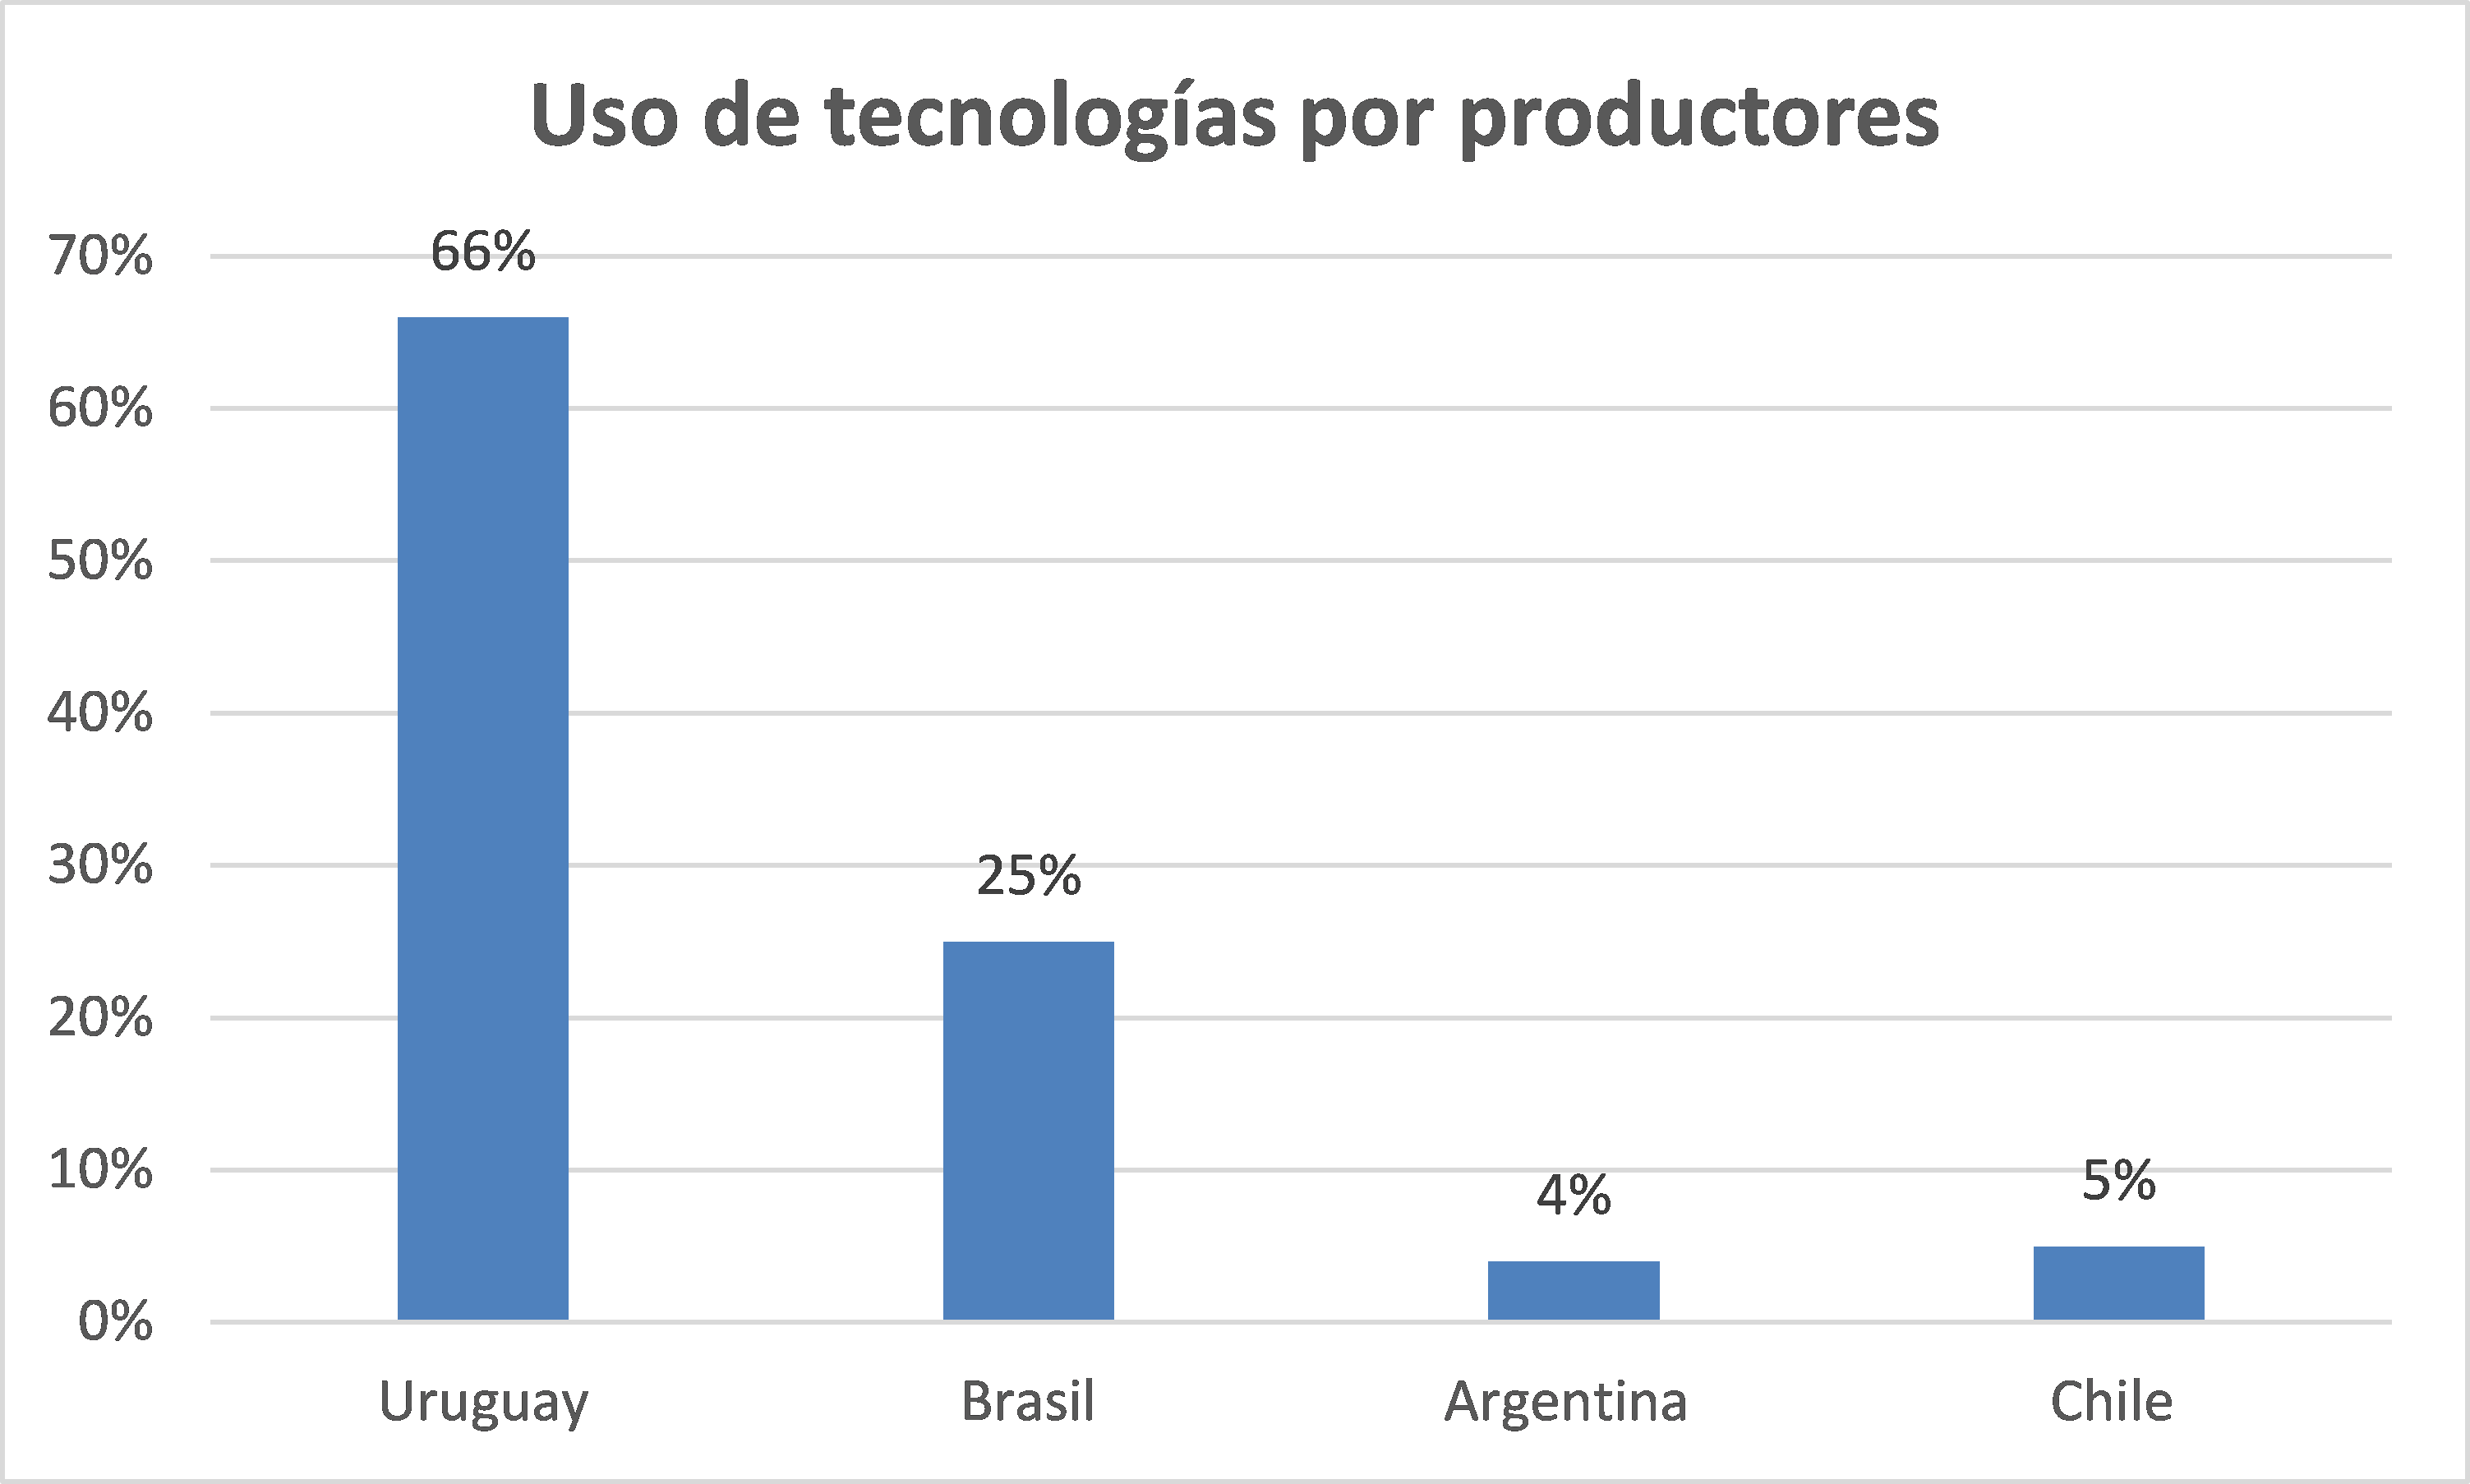
\includegraphics[width=1\textwidth]{usoTecnologias.png}
\caption*{\footnotesize Fuente: Información tomada de FAO \citeyear{fao2021}}
\label{fig:figura1}
\end{figure}

\newpage

El uso de la metodología MLOps en la agricultura ofrece mejoras debido a su capacidad para optimizar la toma de decisiones, automatizar tareas y mejorar la precisión de los resultados de los modelos de machine learning. Esta tecnología puede marcar una gran diferencia en la eficiencia y la sostenibilidad de la agricultura, ayudando a enfrentar los desafíos actuales y futuros del sector.

De allí que, la metodología MLOps tiene un gran potencial para transformar la agricultura y brindar beneficios significativos a los científicos de datos involucrados en esta industria, debido a que pueden aprovechar varias ventajas, como por ejemplo el MLOps permite una mejor gestión de los modelos de aprendizaje automático, es posible utilizar prácticas de control de versiones para rastrear y gestionar los cambios en los modelos, lo que facilita la colaboración y la reproducibilidad de los resultados en las áreas de producción agrícola. Además, el MLOps garantiza un monitoreo continuo de los modelos en producción, lo que permite identificar y solucionar problemas rápidamente.

Al utilizar técnicas de aprendizaje automático, los científicos de datos pueden analizar grandes volúmenes de datos agrícolas para identificar patrones y tomar decisiones informadas, ayudando a implementar estos modelos en sistemas integrados, lo que permite la automatización de tareas agrícolas como el riego, la fertilización y la detección de enfermedades. Esto conduce a un uso más eficiente de los recursos, reduciendo costos y minimizando el impacto ambiental.

En este sentido la tecnología constituye una herramienta relevante para el mundo actual, de allí que este tipo de investigaciones permitan abordar métodos aplicables en la ingeniería de software tanto para la generación de conocimientos, como métodos de aplicación en escenarios reales, como la agricultura y, en particular, el cultivo del aguacate Hass. Asimismo, esta clase de investigaciones abre la vía para la articulación entre los profesionales, las universidades y la industria agrícola para fomentar prácticas económicas y tecnológicas, mejorar y fortalecer actividades de investigación en laboratorios de computación y programas de alfabetización digital, con el objetivo de contribuir al desarrollo económico, científico y académico, asegurando que la ingeniería de software se emplee de forma concreta y provechosa en la solución de problemas prácticos en diversas áreas, como la agricultura.
\newpage

%% Marco conceptual
\section{Marco teórico de referencia y antecedentes}

El marco de referencia está organizado en un primer momento con el análisis del estado del arte para la comprensión del objeto de estudios sobre MLOps para el ámbito agrícola y un segundo momento con los elementos teórico-conceptuales que permiten la argumentación teórica sobre Machine Learning, la metodología MLOps y el cultivo de aguacate Hass con las plagas detalladas para esta investigación.

\subsection{Estado del arte}
Las investigaciones a nivel internacional se describen a continuación:

\begin{longtable}{|p{2cm}|p{3cm}|p{3cm}|p{4cm}|p{3cm}|}

\caption{Investigaciones internacionales}\\
\hline
\textbf{Autor} & \textbf{Título} & \textbf{Objetivo} & \textbf{Metodología} & \textbf{Resultado} \\
\hline
\endhead

\citet{aimacana2021} & Análisis comparativo de algoritmos de Machine Learning para la detección de plagas en los cultivos representativos de la sierra ecuatoriana & Realizar un análisis comparativo entre distintos algoritmos de Machine y Deep Learning, que permita determinar cuál de ellos ofrece mejores resultados en la detección de plagas en cultivos endémicos de la serranía ecuatoriana. & Metodología CRISPDM la cual sus siglas significan Proceso Estándar Entre Industrias para la Minería de Datos. & El estudio realizado se aplicó el mejor modelo para la construcción de un prototipo el cual fue la red neuronal convolucional InceptionV3; el prototipo realizado, permite al usuario enviar imágenes para ser procesadas por el modelo y este a su vez reciba una predicción e información de los síntomas, además de una sugerencia de un posible tratamiento. \\
\hline
\citet{castaneda2021} & Detección de nutrientes del suelo y planta, y pestes en campos de cultivo de banano orgánico con Machine Learning & Diseño una plataforma que sirva de apoyo al agricultor para poder estimar qué macronutrientes tiene en deficiencia su planta de banano, con la finalidad de obtener un mejor producto en la cosecha del banano orgánico, así como una posible interfaz para la detección de plagas en el banano. & Se utilizó un conjunto de fotografías público, el cual fue encontrado en un repositorio y se escogieron aquellas plagas que afectaban al banano. Posteriormente, se realizó un aumento a este conjunto de fotografías mediante transformaciones lineales y las imágenes resultantes fueron pre procesadas en diferentes espacios de color para ser utilizadas como entradas a la red neuronal. & El modelo permitió una alta precisión a través de diferentes métricas. Continuamente se desarrolló un prototipo de plataforma web para que los agricultores en un futuro pudieran acceder al sistema. \\
\hline
\citet{valenzuela2022} & Detección y Clasificación de Enfermedades en el Tomate Mediante Deep Learning y Computer Visión & Aplicar el aprendizaje profundo a problemas de visión de computadora tales como detección y clasificación específicamente en las enfermedades del tomate mediante el procesamiento de imágenes digitales. & Neuronales pre-entrenadas (transfer learning), para hacer la detección de la hoja de tomate (primera: Faster Mask R-CNN) y luego a partir de la detección, realizar la clasificación de la enfermedad (segunda: red neuronal convolucional), tomando como entrada el área de la imagen donde se encuentra la hoja, luego de realizar la clasificación el sistema desarrollado proporciona información de los síntomas asociados a la enfermedad, como también cómo proceder con la prevención y el tratamiento a seguir en tiempo real. & Con el advenimiento de las redes neuronales, ha permitido mejorar drásticamente la precisión, tanto de la detección de objetos como de la clasificación de imágenes. \\
\hline
\citet{garcia2022} & Implementación de modelo Machine Learning aplicado al estudio de enfermedades de café en el centro de investigación Sacha Wiwa, perteneciente a la parroquia Gasaganga, Cantón la Maná, provincia de Cotopaxi & Implementar modelo de clasificación de imágenes empleando técnicas de Machine Learning, para la detección de enfermedades del Cafeto (Coffea arábica) en huertas del Centro de Investigación Sacha Wiwa. & Cualitativa experimental permite la selección, análisis y presentación de los datos documentados de una manera ordenada y siguiendo los objetivos del proyecto. & Mediante el modelo de Machine Learning desarrollado en el entorno virtual “Jupyter lab” se lograron crear y entrenar las redes neuronales convencionales para la clasificación de las enfermedades del café expuestas en el caso de estudio en conjunto con la clasificación sana del cafeto. \\
\hline
\caption*{\footnotesize Fuente: Elaboración propia}
\end{longtable}


En las investigaciones a nivel internacional se pude observar que el desarrollo de Machine Learning, en particular el uso de redes neuronales, ha demostrado ser de gran importancia en el control de plagas y enfermedades en diversos campos, como la agricultura, asimismo este utiliza un modelo de red neuronal convolucional para la detección de plagas y enfermedades como por ejemplo en los cultivos de  café,  tomate y banano donde es un ejemplo claro de cómo el Machine Learning puede contribuir al control de plagas.

Uno de los principales beneficios del Machine Learning en el control de plagas es su capacidad para analizar grandes volúmenes de datos y extraer patrones y características relevantes, en las investigaciones se observaron que utilizaban imágenes  de plantas enfermas como sanas, lo que le permitió aprender a reconocer los síntomas y distinguir entre diferentes enfermedades. Esto es especialmente útil en el control de plagas, ya que puede facilitar la detección temprana de enfermedades y ayudar a los agricultores a tomar medidas preventivas o correctivas de manera oportuna.

Para el caso de las investigaciones nacionales se detallan en la siguiente tabla:


\begin{longtable}{|p{2cm}|p{3cm}|p{3cm}|p{4cm}|p{3cm}|}

\caption{Investigaciones a nivel nacional}\\
\hline
\textbf{Autor} & \textbf{Título} & \textbf{Objetivo} & \textbf{Metodología} & \textbf{Resultado} \\
\hline
\endhead

\hline
\endfoot

\hline
\endlastfoot

\citet{tovar2019} & Diseño e implementación de un aplicativo móvil para realizar la detección temprana de la enfermedad de la Sigatoka Negra en los cultivos de plátanos & Diseñar e implementar un aplicativo móvil, para realizar la detección temprana de la enfermedad de la Sigatoka Negra en los cultivos de plátanos. & La metodología utilizada para la detección de esta enfermedad, consistió en construir una base de datos que contiene imágenes de los posibles estados de la misma, teniendo en cuenta la escala estándar de Fouré utilizada para analizar la forma de evolución de la Sigatoka Negra. Luego se inició con la creación del algoritmo, en donde se realizó la segmentación de cada una de las imágenes para generar un realce en la enfermedad, para posteriormente obtener las características respectivas y finalmente a partir de las técnicas de Machine Learning generar una clasificación que identifique el estadío en el que se encuentra una hoja al tomar una imagen que no se ubique dentro de la base de datos. & El aplicativo móvil demostró un porcentaje de acierto del 80\% en la detección de la Sigatoka Negra. Por lo tanto, la aplicación puede llegar a ayudar a los productores de plátano, evitando así pérdidas económicas. \\
\citet{avila2022} & Entrenamiento de redes neuronales para la identificación de plagas en cultivos de café. & Implementar un aplicativo basado en visión artificial para la identificación de Cercospora, Phoma, Roya, minador de hojas y Arañita roja, en el café a partir del análisis de las hojas de la planta. & Esta base será introducida a modelos de redes neuronales: densa, neuronal convolucional y neuronal convolucional con overfitting, usando el lenguaje Python y las bibliotecas: Keras y TensorFlow. Una vez entrenado el modelo, se procede al análisis de las imágenes que contienen la morfología de la planta y que servirán de entrada a una red neuronal para poder comparar los resultados y determinar cuál de los modelos presenta mejores resultados. & El modelo convolucional con overfitting presenta el mejor resultado de predicción, pero aun así, es un modelo limitado que podría ser reemplazado por otros modelos de mayor alcance, como ResNet50, CIFAR-10, VGG19. Al tener una cantidad de plagas tan limitada, es evidente que no se puede hacer un reconocimiento más detallado de las plagas, por lo que sería necesaria ampliar la base de datos \\
\hline
\caption*{\footnotesize Fuente: Elaboración propia}
\end{longtable}

A nivel nacional los diferentes modelos operativos en el contexto de la detección de plaga hace referencia a un modelo convolucional con overfitting que presenta los mejores resultados de predicción, pero se plantea la posibilidad de reemplazarlo por otros modelos de mayor alcance, como ResNet50, CIFAR-10 o VGG19.

La elección del modelo operativo es crucial en cualquier aplicación de Machine Learning, ya que tiene un impacto directo en la precisión y el rendimiento del sistema. En el caso mencionado, el modelo convolucional con overfitting logró un alto nivel de acierto en la detección de plaga.

\subsection{Bases teóricas}
\subsubsection{Metodología MLOps}

Machine Learning Operations (en sus siglas en ingles MLOps) es un conjunto de prácticas que combinan Machine Learning, DevOps e Ingeniería de datos, cuyo objetivo es implementar y mantener sistemas ML en producción de manera confiable y eficiente.
 
En esa dirección Rivero (\citeyear{rivero2022}) explica que, MLOps se refiere a las prácticas y metodologías que permiten gestionar y optimizar el ciclo de vida de los sistemas de aprendizaje automático (Machine Learning) de forma que se puede desarrollar confiablemente. Se tiene en cuenta que, la metodología MLOps combina técnicas y herramientas de desarrollo de software con conocimientos de ciencia de datos y operaciones de infraestructura, para permitir la implementación, el monitoreo y el mantenimiento escalable de los modelos de aprendizaje automático en producción.

En el contexto del desarrollo de modelos de Machine Learning, MLOps aborda los desafíos asociados con la gestión de datos, la experimentación, el entrenamiento, la implementación, el monitoreo y la reevaluación continua del rendimiento del modelo, que lo hacen diferente a DevOps y la Ingenieria de Datos como se describe en la Tabla \ref{tab:practicas}. Esto implica el uso de técnicas como la integración y entrega continua (CI/CD), la orquestación de flujos de trabajo, la automatización de pruebas y la gestión de versiones.

\begin{table}[h]
\centering
\caption{Comparativo entre DevOps, Ingeniería de Datos y MLOps}
\label{tab:practicas}
\begin{tabular}{|p{3cm}|p{3cm}|p{3cm}|p{4cm}|}
\hline
\textbf{Práctica} & \textbf{DevOps} & \textbf{Ingeniería de Datos} & \textbf{MLOps} \\
\hline
Control de versiones & Versionamiento de código & Versionamiento de código linaje de datos & Versionamiento de código + datos + modelos (conectados) \\
\hline
Pipeline & n/a & Flujo de datos/ETL & Flujo de ML de entrenamiento, flujo de ML para predicción \\
\hline
Validación de comportamiento & Pruebas unitarias & Pruebas unitarias & Validación de modelo \\
\hline
CI/CD & Despliegue de código en producción & Despliega código en flujo de datos & Despliegue de código a producción + Flujo de datos de ML \\
\hline
Validación de datos & n/a & Validación de negocio y formato & Validación estadística \\
\hline
Monitoreo & Basados en SLOs & Basados en SLOs & SLOs + monitoreo diferencial y estadístico \\
\hline
\end{tabular}
\caption*{\footnotesize Fuente: \citet{rivero2022}}
\end{table}

\newpage

El objetivo fundamental de MLOps es garantizar que los modelos de aprendizaje automático sean confiables, reproducibles y escalables en entornos de producción. Al adoptar prácticas de MLOps, las organizaciones pueden acelerar el tiempo de comercialización de sus modelos, mejorar la colaboración entre equipos multidisciplinarios, minimizar los riesgos asociados con los modelos en producción y facilitar la implementación de mejoras y actualizaciones. Estos avances en la metodología MLOps se vienen desarrollando desde el año 2000 para resolver los distintos problemas para los contextos ML (ver figura \ref{fig:figura2}).\\


\begin{figure}[h]
\caption{Evolución temporal de MLOps}
\centering
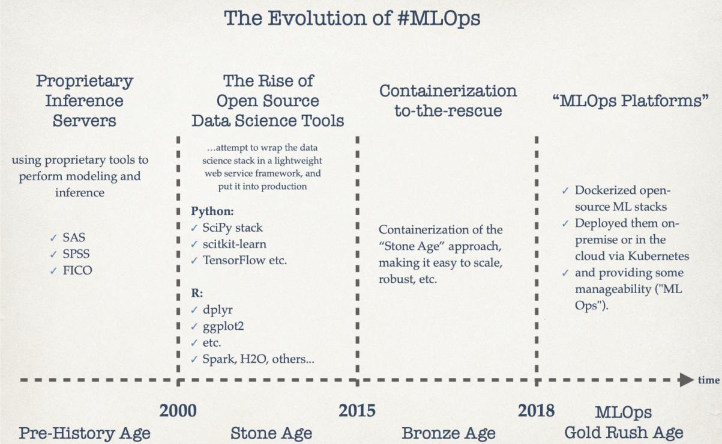
\includegraphics[width=1\textwidth]{evolucionTemporalMLOPS.png}
\label{fig:figura2}
\caption*{\footnotesize Fuente: \citet{visengeriyeva2020}}
\end{figure}


\newpage
La metodología MLOps es una disciplina que fusiona las mejores prácticas de desarrollo de software con los desafíos específicos del Machine Learning, con el objetivo de facilitar la implementación y gestión de modelos de aprendizaje automático. Con el auge del software de código abierto y la disponibilidad de datos, más profesionales de software comenzaron a usar bibliotecas Python o R para entrenar modelos ML. 

A medida que iba surgiendo la tecnología de contenerización, se resolvió el despliegue del modelo de forma escalable mediante el uso de contenedores Docker y Kubernetes. Recientemente, vemos la evolución de esas soluciones hacia plataformas de implementación de ML que cubren toda la iteración de experimentación, capacitación, implementación y monitoreo de modelos \citep{visengeriyeva2020}.
\newpage

\textbf{Proceso de la metodología MLOps}
\begin{itemize}
\item \textbf{Flujos de ML:} Los flujos de datos, también llamados pipelines de datos o procesos ETL (extraer, transformar y cargar), son procesos donde los datos son obtenidos desde una fuente, para ser transformada y luego cargada en la misma fuente o en otro sistema. Las transformaciones de los datos se refieren a todos los cambios necesarios sobre los mismos, para que queden con el formato que es requerido en el destino final (el modelo de ML).
\item \textbf{Versionado de modelos y de datos:} En aprendizaje automático es igual de importante mantener registro de las diferentes versiones del código, pero se le suma también la necesidad de registrar las versiones del modelo, así como de los datos que fueron utilizados para entrenarlo, y de otros datos como hiper-parámetros del modelo.
\item \textbf{Validación de modelos:} Se debe tener en cuenta:
    \begin{enumerate}
        \item \textbf{Precisión del modelo:} de los casos que el modelo clasificó como verdaderos positivos (TP).
        \item \textbf{Recall del modelo:} la precisión abierta por categorías.
        \item \textbf{Medición de sesgo en los datos:} es importante realizar mediciones que ayuden a entender si el modelo está sesgado.
        \item \textbf{Casos críticos:} un modelo puede tener buena precisión, exhaustividad(recall) y no estar sesgado, pero no tomar los casos más importantes en la historia reciente.
        \item \textbf{Medición de un modelo de regresión:}\\
- Métricas globales del modelo como RMSE, MAE Y R2.\\
- Las mismas métricas pero aperturadas por diferentes cortes, para entender si hay algún segmento en el cual el modelo tenga oportunidades de mejora.\\
- Medición del sesgo en los datos, igual que en los problemas de clasificación.\\
- Casos críticos, igual que en los problemas de clasificación.
    \end{enumerate}
\item \textbf{Validación de datos:} Se genera en dos pasos, el primero corresponde al más básico es la calidad de los mismos, lo cual incluye verificar cantidad de nulos, el SLA (service level agreement) de actualización de los datos, que todos los datos sean del tipo esperado, entre otros. El segundo es el más complejo consiste en monitorear la distribución de los datos. Un cambio en la distribución puede ser originada por una falla en alguno de los pipelines o por cambios en los datos \citep{rivero2022}. 
\end{itemize}

Entre las diversas herramientas disponibles para el MLOps, se pueden clasificar en dos categorías distintas: las sencillas y las complejas. Las herramientas sencillas son particularmente útiles para facilitar el despliegue local, es decir, en un mismo ordenador o un servidor local. Este enfoque es especialmente adecuado para equipos pequeños de investigación, donde estos miembros del equipo pueden acceder desde diferentes computadoras de manera local. Estas herramientas sencillas representan el primer paso para llevar la solución a la fase de despliegue, especialmente en entornos de producción.

Por otro lado, las herramientas complejas están diseñadas para gestionar mayores capacidades de cómputo. Estas pueden configurarse con capacidades específicas, e incluso el sistema puede autoajustarse según el tráfico y los requisitos de almacenamiento, incorporando la funcionalidad conocida como ``On Demand'', donde son capaces de autoescalar según las necesidades del momento. 

Después de implementar las herramientas sencillas, se puede aprovechar lo creado para desplegar una aplicación. Esta aplicación, inicialmente desarrollada o creada localmente, puede integrarse con uno de los servicios en la nube más comunes y populares. Estos servicios en la nube, como AWS, Azure, GCP, son seleccionados debido a su amplia cuota de mercado y su uso generalizado en la actualidad. Esto permite llevar la aplicación creada localmente a aprovechar las capacidades y escalabilidad que ofrecen los servicios en la nube para su despliegue.

\newpage

La implementación de un monitoreo completo plantea ciertas consideraciones, especialmente cuando se considera la adopción de herramientas complejas. La complejidad de estas herramientas conlleva un aumento en los costos, ya que se aplican cargos por el conjunto completo de funcionalidades que ofrecen. En comparación, al optar por el uso de herramientas sencillas locales y utilizar solo una fracción de las herramientas complejas resulta más económico.

Además del aspecto financiero, es crucial tener en cuenta que el uso de herramientas complejas implica una curva de aprendizaje significativa. Se requiere una inversión de tiempo y esfuerzo para adquirir los conocimientos necesarios y comprender cómo manipular eficazmente todo el ciclo del MLOps. Esta curva de aprendizaje elevada puede representar una desventaja, ya que impone una barrera para aquellos que buscan implementar estas herramientas de manera efectiva.

En general, se han ido desarrollando muchas herramientas que se pueden utilizar para implementar la metodología de MLOps tanto de acceso libre (open source) o de pago, para usar localmente o desde internet. Y se deben escoger cada una con base a las necesidades del proyecto.

\begin{figure}[h]
	\centering
	\caption{Herramientas que implementan ciclo completo de MLOps}
	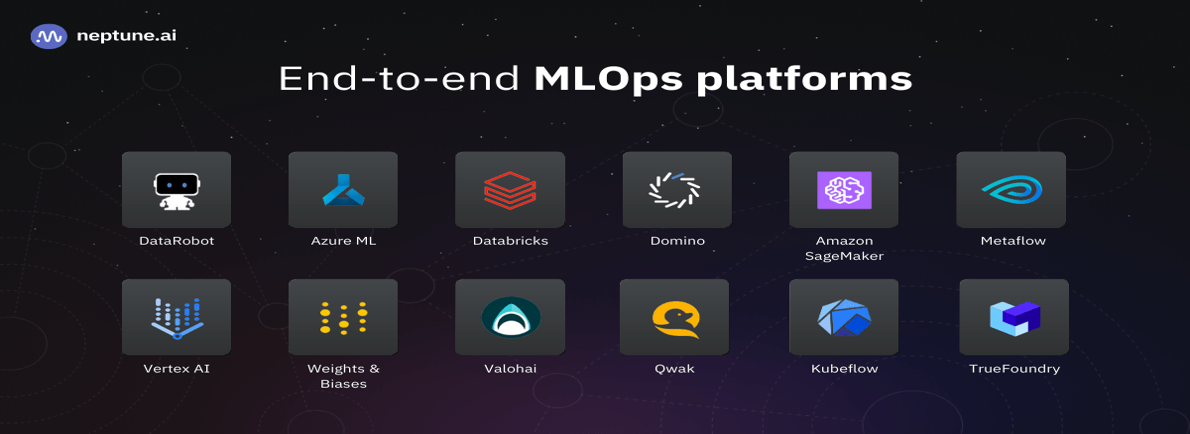
\includegraphics[width=0.8\textwidth]{resultados/herramientasMLOps.png}
	\caption*{\footnotesize Fuente: \cite{neptune2024}}
	\label{fig:figuraHerramientasMLOps}
\end{figure}

\newpage

Dentro de las plataformas descritas en la imagen anterior (ver figura \ref{fig:figuraHerramientasMLOps}) se encuentra MetaFlow, esta plataforma en sí misma, es una herramienta gratuita, aunque algunas de sus funcionalidades pueden requerir pagos. Por ejemplo, el despliegue en internet podría estar sujeto a tarifas adicionales. Para completar todo el ciclo de vida del MLOps, es necesario considerar diversas herramientas, muchas de las cuales ofrecen características completas o parciales para gestionar eficazmente este ciclo.

\begin{figure}[h]
	\centering
	\caption{Herramientas de análisis de datos y repositorio de código}
	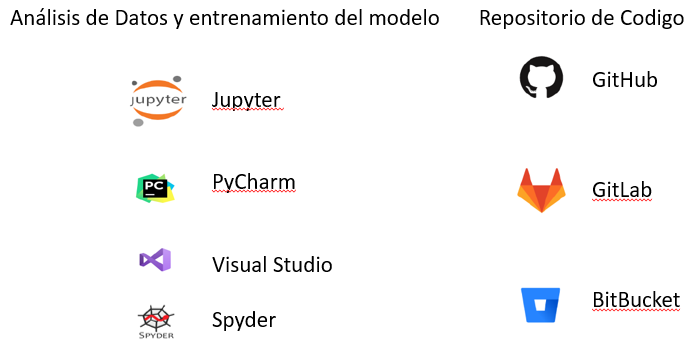
\includegraphics[width=0.7\textwidth]{resultados/herramientasAnaRepo.png}
	\caption*{\footnotesize Fuente: Elaboración propia}
	\label{fig:figuraHerramientasAnaRepo}
\end{figure}

\newpage

\begin{figure}[h]
	\centering
	\caption{Herramientas de registro de modelo, versionado del modelo y versionado de datos}
	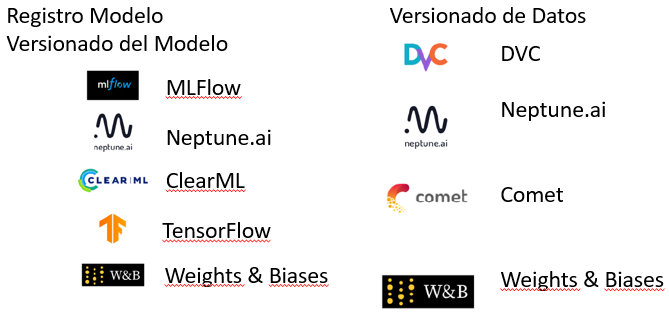
\includegraphics[width=0.7\textwidth]{resultados/herramientasRegModDatos.png}
	\caption*{\footnotesize Fuente: Elaboración propia}
	\label{fig:figuraHerramientasRegModDatos}
\end{figure}

\begin{figure}[h]
	\centering
	\caption{Herramientas para Construcción de API y Construcción de aplicación Web}
	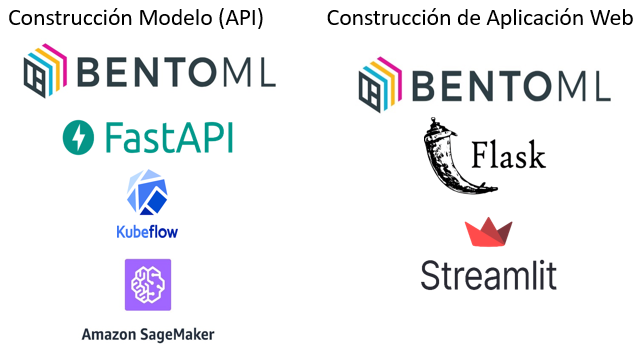
\includegraphics[width=0.6\textwidth]{resultados/herramientasDespApiApp.png}
	\caption*{\footnotesize Fuente: Elaboración propia}
	\label{fig:figuraHerramientasDespApiApp}
\end{figure}

\newpage

\begin{figure}[h]
	\centering
	\caption{Herramientas de Feature Store y Monitoreo del Modelo}
	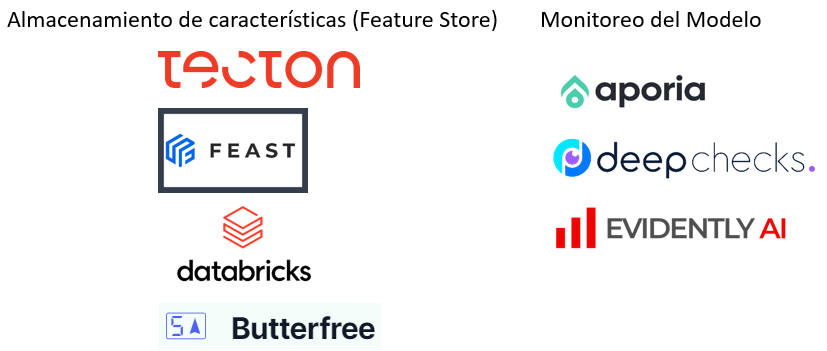
\includegraphics[width=0.9\textwidth]{resultados/herramientasFeaMon.png}
	\caption*{\footnotesize Fuente: Elaboración propia}
	\label{fig:figuraHerramientasFeaMon}
\end{figure}

Continuando con el tema, centrémonos ahora en las herramientas que simplifican los despliegues de una aplicación o una API de manera automatizada. La necesidad de estas herramientas radica en lo tedioso que implicaría realizar despliegues manualmente. En un enfoque manual, se tendría que especificar la imagen que debe utilizarse desde un contenedor, crear el contenedor, y posteriormente enviarlo a la nube. Luego, sería necesario obtener la URL para su uso. Este proceso, aunque es posible de realizar manualmente, se vuelve más eficiente y menos propenso a errores al utilizar herramientas como GitHub Actions, la cual es una herramienta de automatización integrada con GitHub.

Algunas características clave y conceptos asociados con GitHub son:

\begin{itemize}
	\item \textbf{Repositorios:} Son espacios donde se almacenan los archivos de un proyecto,  junto  con  la  información  de  seguimiento  de  versiones.  Cada  proyecto  en GitHub se guarda en un repositorio.
	\item \textbf{Control de Versiones:} GitHub utiliza Git, un sistema de control de versiones distribuido. Esto significa que cada desarrollador o miembro de un equipo, que trabaja en un proyecto tiene una copia completa del historial de cambios del proyecto en su  máquina  local.  Git  permite  rastrear  cambios,  fusionar  contribuciones  y  revertir  a versiones anteriores del código.
	\item \textbf{Automatización:} GitHub Actions es un servicio que permite a los ingenieros de software automatizar diversas tareas en respuesta a eventos específicos dentro del repositorio. En el contexto del proyecto, las tareas se configuran mediante flujos de trabajo definidos en archivos YAML. Estos flujos de trabajo simplifican la ejecución de pruebas, la construcción de una API o una aplicación, junto con los despliegues. GitHub Actions no solo facilita la automatización de estos procesos, sino que también respalda la integración continua y el despliegue continuo.
	
	Esta integración automatizada con GitHub Actions no solo agiliza el ciclo de desarrollo, sino que también asegura la coherencia y confiabilidad en el proceso de despliegue de una aplicación o una API. Con esta herramienta, se logra una gestión eficiente y automatizada de todo el ciclo de vida del modelo para llevarlo a producción, desde la integración de cambios hasta la entrega y despliegue en un proveedor de servicios en la nube.
\end{itemize}

\subsection{Modelo de Machine Learning}

De acuerdo con Murphy (\citeyear{murphy2012}), el modelo Machine Learning se refiere a la localización automatizada de datos que se encuentran estandarizados, además es una herramienta constante en el proceso de extracción de grandes volúmenes de información para su organización y análisis, definido también como Big Data. En la actualidad el Machine Learning se encuentra en los motores de búsqueda con los cuales se desarrollan resultados instantáneos como por ejemplo los anuncios, software antispam, las transacciones con la tarjeta de crédito, etc.

Estas nuevas tecnologías, a través del internet, permiten la recopilación de bases de datos de un tamaño considerable, pueden ser históricos o datos en tiempo real, siendo posible el análisis de datos debido a las mejoras constantes en la tecnología y el desarrollo de software. Para Shalev y Ben (\citeyear{shalev2014}), este desarrollo ha permitido que las bases de datos se encuentren en distintos formatos, lo que es un desafío para orientar estrategias que permitan resolver distintos problemas de acuerdo a las necesidades de cada formato y de esta manera avanzar en el desarrollo de métodos para el Machine Learning.

El Machine Learning al ser un proceso automatizado que retoma patrones en grandes cantidades de datos, permitiendo la implementación de modelos que utilizan aplicaciones de análisis de datos predictivos, teniendo en cuenta:

    \begin{enumerate}
        \item Técnicas de aprendizaje automático siendo un modelo de la relación entre un conjunto de características descriptivas y una característica objetivo basado en un conjunto de ejemplos históricos o instancias comunes.
        \item Posteriormente, es posible con este modelo establecer nuevas predicciones de manera constante \citep{shalev2014}.
    \end{enumerate}

Por esta razón con el Machine Learning es posible establecer tres tipos de modelos el geométrico, el probabilístico y el lógico (ver tabla \ref{tab:modelos}) y tres tipos de aprendizajes: el supervisado, el no supervisado y semi-supervisado (ver tabla \ref{tab:tipos}), ya que se busca el aprendizaje continuo, conocer el progreso y la veracidad de la información que se desarrolla, porque:

\begin{quote}
    "Su aplicación está determinada en diferentes ámbitos dependiendo de las necesidades del problema, permitiendo a los científicos y especialistas tomar decisiones referentes a temas tan puntales como si un tipo de material puede ser separado por características de resistencia a la fragmentación o capacidad de absorción de energía pudiendo determinar con esto si es recomendable su uso en una u otra tarea específica" \citep[p.42]{salamanca2021}.
\end{quote}

\begin{table}[htbp]
\centering
\caption{Modelos para el desarrollo de Machine Learning}
\label{tab:modelos}
\begin{tabular}{|l|p{10cm}|}
\hline
\textbf{Modelo} & \textbf{Características} \\
\hline
Geométrico & El espacio de instancias abarca la totalidad de las configuraciones concebibles, ya sea que estén representadas en nuestro conjunto de datos o no. Suele exhibir una estructura geométrica definida. Por ejemplo, cuando todas las características son de naturaleza numérica, cada una puede interpretarse como una coordenada en un sistema cartesiano. \\
\hline
Probabilístico & Numerosos modelos se sustentan en el siguiente concepto fundamental: Consideremos X como las variables que describen, por ejemplo, las características de una instancia conocida; mientras que Y representa las variables objetivo que nos conciernen, como la clase a la que pertenece dicha instancia. La esencia del aprendizaje automático radica en la capacidad de modelar la interrelación entre X e Y. \\
\hline
Lógico & Toma su inspiración de disciplinas como la informática y la ingeniería. Se denomina ``lógico" debido a que sus modelos pueden ser traducidos de manera sencilla en reglas comprensibles para los seres humanos, por ejemplo: \begin{verbatim}
if Viagra=1 then Class=Y=spam
\end{verbatim} \\
\hline
\end{tabular}
\caption*{\footnotesize Fuente: \citet[p.~43]{salamanca2021}}
\end{table}

\begin{table}[htbp]
\centering
\caption{Los tipos de aprendizaje en el ML}
\label{tab:tipos}
\begin{tabular}{|p{4cm}|p{10cm}|}
\hline
\textbf{Tipos} & \textbf{Fundamento} \\
\hline
Aprendizaje supervisado & Consiste en encontrar el mejor clasificador posible $f: X \rightarrow Y$ para un problema determinado. El algoritmo responsable de encontrar este mapeo se denomina algoritmo de clasificación, que infiere un modelo de cada ejemplo de entrada $x \in X$ y su respectiva clase $y \in Y$. Este modelo es una aproximación para la distribución de probabilidad conjunta (DPC) de las variables $X$ e $Y$. \\
\hline
Aprendizaje no supervisado & Son aquellos en los que no estamos interesados en ajustar pares (entrada, salida), sino en aumentar el conocimiento estructural de los datos disponibles (y posibles datos futuros que provengan del mismo fenómeno), por ejemplo, dando una agrupación de los datos según su similaridad (clustering), simplificando las estructura de los mismos manteniendo sus características fundamentales (como en los procesos de reducción de la dimensionalidad), o extrayendo la estructura interna con la que se distribuyen los datos en su espacio original (aprendizaje topológico). \\
\hline
Aprendizaje semi supervisado & El objetivo es la clasificación, pero la entrada contiene datos etiquetados y sin etiquetar. El aprendizaje semi-supervisado, debido a su estructura, se puede dividir principalmente en dos tipos, según el objetivo del análisis que se busque hacer a la base de datos:
\begin{minipage}[t]{\linewidth}
    \begin{enumerate}
      \item Aprendizaje transductivo, que separa el conjunto dado en conjunto de entrenamiento (donde la variable objetivo es conocida), y conjunto de prueba donde ésta no es dada.
      \item Aprendizaje inductivo trata de obtener una función de predicción usando todo el conjunto $\{(X, Y)\}$, es decir, usando tanto los datos donde la variable objetivo es conocida como aquellos en los que no.
    \end{enumerate}
\end{minipage} \\
\hline
\end{tabular}
\caption*{\footnotesize Fuente: \citet[p.~44-45]{salamanca2021}}
\end{table}

\newpage
Autores como \citet{contreras2022}, \citet{salamanca2021} y \citet{jara2016} explican que, en el campo del Machine Learning los métodos de predicción presentan un papel fundamental al permitir que las máquinas realicen predicciones precisas sobre datos no vistos. Existen varios métodos utilizados en el Machine Learning para generar predicciones, entre ellos se destacan los siguientes:

\begin{enumerate}
    \item Regresión: Es utilizado para predecir un valor numérico continuo basado en variables independientes. Algunos ejemplos comunes son la regresión lineal y la regresión logística, que se utilizan para predecir la relación entre variables \citep{salamanca2021}.
    \item Clasificación: Se utiliza para predecir la pertenencia a una clase o categoría específica. Los algoritmos de clasificación, como el árbol de decisiones, las máquinas de vectores de soporte (SVM) y los clasificadores de Naive Bayes, se emplean para clasificar datos en categorías predeterminadas \citep{salamanca2021}.
    \item Agrupamiento: Es utilizado para agrupar conjuntos de datos similares en clusters o grupos. Algunos métodos comunes de agrupamiento son el algoritmo k-means y el agrupamiento jerárquico, que ayudan a encontrar patrones y estructuras ocultas en los datos \citep{contreras2022}.
    \item Redes neuronales: Estas técnicas se basan en modelos inspirados en el funcionamiento del cerebro humano. Las redes neuronales profundas, como las redes neuronales convolucionales (CNN) y las redes neuronales recurrentes (RNN), han logrado grandes avances en áreas como la visión por computadora y el procesamiento del lenguaje natural \citep{salamanca2021}.
\end{enumerate}

Estos métodos de predicción en el Machine Learning han demostrado ser eficientes en una amplia gama de aplicaciones, desde la detección de fraudes hasta el diagnóstico médico y la recomendación de productos. La elección del método adecuado depende del tipo de datos, el problema a resolver y los objetivos específicos del proyecto de Machine Learning. Para verificar su eficiencia, estos métodos deben ser validados por una matriz de confusión la cual contiene:

\begin{figure}[h]
	\centering
	\caption{Matriz de confusión para la evaluación de los modelos}
	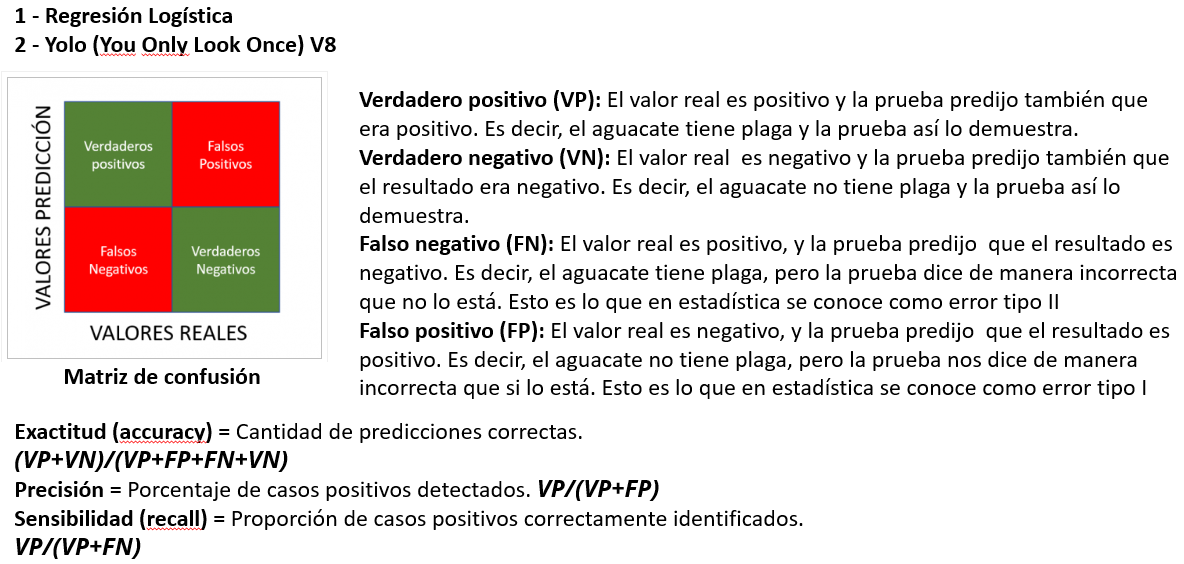
\includegraphics[width=1\textwidth]{resultados/evaModelos.png}
	\caption*{\footnotesize Fuente: Elaboración propia}
	\label{fig:figuraEvaModelos}
\end{figure}

\newpage


\subsubsection{Cultivo de aguacate Hass}

El cultivo del aguacate HASS es cada vez más popular en la agricultura debido a sus características y beneficios. El aguacate HASS es una variedad de aguacate que se distingue por su adaptabilidad a diferentes condiciones climáticas y su alta productividad. Según estudios realizados por el Departamento Administrativo de Nacional de Estadística \citep{dane2016cultivo}, esta variedad se ha destacado por su resistencia a enfermedades y plagas comunes en el cultivo del aguacate.

Una de las ventajas de cultivar el aguacate Hass es su capacidad para adaptarse a diferentes climas, según los autores \citet{reyes2022}, esta variedad es apta para regiones con temperaturas que oscilan entre los 10 y 35 grados Celsius, además, puede tolerar tanto condiciones secas como húmedas, lo que la convierte en una opción viable para diferentes áreas geográficas.

Cabe destacar, que  otra de las características  del aguacate Hass es su alta productividad, esta variedad puede alcanzar rendimientos superiores a los 20 kilogramos de fruta por árbol al año, esto la convierte en una opción rentable para los agricultores, ya que pueden obtener una mayor producción por unidad de superficie cultivada \citep{reyes2022}.

Además de su adaptabilidad y productividad, el aguacate Hass presenta resistencia a enfermedades comunes en el cultivo del aguacate, según los autores \citet{agapito2022}, esta variedad ha mostrado resistencia al hongo Phytophthora cinnamomi, causante de la pudrición de raíz, lo que reduce la necesidad de aplicar productos químicos para su control.

\subsubsection{Plagas Stenoma catenifer y heilipus lauri}

El cultivo del aguacate puede verse amenazado por diversas plagas que pueden afectar tanto las hojas, los frutos como las raíces de la planta, según  el Dane  (\citeyear{dane2016cultivo}) las plagas más comunes son el ácaro del aguacate entre los que se encuentran el \textit{Heilipus lauri} y el \textit{Stenoma catenifer}, quienes provoca un daño en la apariencia de la planta y puede reducir su capacidad de fotosíntesis, para controlar esta plaga, se pueden emplear insecticidas específicos o realizar una poda adecuada de las hojas afectadas.

Para \citet{carabali2022}, en el cultivo del aguacate Hass la \textit{Stenoma catenifer} (ver figura \ref{fig:figuraStenoma}) desarrolla su polilla al alimentarse de los frutos del aguacate, perforando galerías y causando daños considerables en la calidad de la cosecha. Asimismo la plaga del barrenador del hueso del aguacate \textit{Heilipus} spp (ver figura \ref{fig:figuraHeilipus}), puede causar daños graves al cultivo, las  larvas de este insecto se alimentan del interior del hueso del aguacate, lo que afecta el desarrollo adecuado del fruto \citep{carabali2022}.

\begin{figure}[h]
\centering
\caption{Fotografía del insecto Stenoma catenifer}
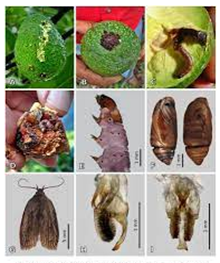
\includegraphics[width=0.5\textwidth]{stenoma.png}
\caption*{\footnotesize Fuente: \cite{diaz2017}}
\label{fig:figuraStenoma}
\end{figure}

\begin{figure}[h]
\centering
\caption{Fotografía del insecto Heilipus lauri}
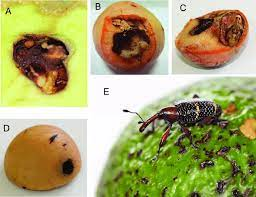
\includegraphics[width=0.5\textwidth]{heilipusLauri.png}
\caption*{\footnotesize Fuente: \cite{palacios2011}}
\label{fig:figuraHeilipus}
\end{figure}
\newpage

%% Metodología
\section{Metodología de la investigación}
La metodología exploratoria aplicada es un enfoque de investigación que se utiliza para explorar y comprender fenómenos o problemas que son poco conocidos o no han sido investigados previamente de manera exhaustiva \citep{zafra2006}. Se emplea cuando existe una falta de información o teorías bien establecidas sobre el tema de estudio, como lo son la identificación y monitoreo de plagas en el cultivo de aguacate Hass a través de metodologías MLOps.

De acuerdo con Zafra (\citeyear{zafra2006}), la metodología exploratoria aplicada es flexible y adaptable, permitiendo a los investigadores ajustar su enfoque a medida que se obtiene nueva información. Al principio del proceso, el investigador puede tener una comprensión limitada del fenómeno, pero a medida que avanza la investigación, se van generando nuevas preguntas e ideas que guían el proceso de recolección y análisis de datos.

La metodología exploratoria aplicada fue un enfoque flexible y creativo que permitió a los investigadores en ingeniería de software explorar y comprender fenómenos como el Big Data y las metodologías MLOps que son relativamente nuevos para generar conocimiento y a establecer las bases para investigaciones futuras más rigurosas y proporciona una base sólida para futuras investigaciones y puede contribuir a generar explicaciones y enfoques más avanzados en relación con la producción agrícola.

El estudio se llevó a cabo en cuatro huertos comerciales de aguacate Hass que se encuentran ubicados en los municipios de Sotará y Timbío del departamento del Cauca, donde existe un impacto considerable de las plagas \textit{Stenoma catenifer} y \textit{heilipus lauri} \citep{zapata2022}. Esta situación de plagas analizada cuenta con una amplia base de datos fotográficas que serán procesadas para esta investigación.

De allí que se oriente la investigación con las siguientes fases metodológicas que permitan dar cumplimiento al proyecto:

\textbf{Fase I:} Para el objetivo de implementar técnicas de procesamiento de imágenes para extraer características relevantes y mejorar la capacidad del modelo de Machine Learning en el reconocimiento y detección de las plagas \textit{Stenoma catenifer} y \textit{heilipus lauri} en el cultivo de aguacate Hass a partir de imágenes capturadas en campo:
\begin{itemize}
    \item Recopilar datos e imágenes que permitan una base de datos para reconocer las características propias de plantas con y sin plagas.
    \item Procesar los datos e imágenes de la plantación de café donde se desarrolla el proceso de redimensionar las imágenes, normalizar los valores de los píxeles y elimina los posibles errores de imagen.
    \item Realizar técnicas de segmentación para aislar las regiones relevantes que contienen la planta de café.
\end{itemize}

\textbf{Fase II:} El objetivo es desarrollar y entrenar un modelo de Machine Learning utilizando técnicas apropiadas de preprocesamiento y selección de características, así como algoritmos de aprendizaje supervisado o no supervisado, para lograr una detección de las plagas \textit{Stenoma catenifer} y \textit{heilipus lauri} en el cultivo de aguacate Hass.
\begin{itemize}
    \item Dividir el conjunto de datos preprocesado en un conjunto de entrenamiento y un conjunto de prueba.
    \item Realizar la implementación de los pipelines necesarios para la automatización de las tareas de encapsulamiento y despliegue.
    \item Utilizar el conjunto de entrenamiento para entrenar el modelo seleccionado donde  el modelo asimilará el reconocimiento de los patrones asociados con y sin las plagas.
\end{itemize}

\textbf{Fase III:} En el objetivo desarrollar una metodología MLOps que permita la integración, automatización y monitoreo del modelo de Machine Learning diseñado para el reconocimiento y control de las plagas \textit{Stenoma catenifer} y \textit{heilipus lauri} en el cultivo de aguacate Hass:
\begin{itemize}
    \item Seleccionar el modelo de Machine Learning para la detección de objetos en imágenes.
    \item Utilizar técnicas como el filtrado, detección de bordes, extracción de texturas y características específicas de las plagas que desees detectar en el modelo.
\end{itemize}

\textbf{Fase IV:} En el objetivo validar el uso de MLOps mediante despliegue en un ambiente controlado, con la capacidad de monitorear y mejorar continuamente el rendimiento del modelo.
\begin{itemize}
    \item Evaluar el modelo utilizando el conjunto de prueba y ajustarlos a los parámetros y a la arquitectura del modelo según sea necesario para mejorar su rendimiento.
    \item Observar el rendimiento del conjunto de prueba para desplegarlo en tiempo real en aplicaciones de detección de plagas.
\end{itemize}

Todo este proceso se realizó aplicando los principios fundamentales de MLOps, siguiendo las medidas de seguridad informática requeridas para salvaguardar los datos personales, y además, cumpliendo con el conjunto de mejores prácticas en el desarrollo de software en general.
\newpage

%% Recursos
%%\section{Recursos a emplear}
A continuación, se resumen los recursos necesarios para llevar a cabo la propuesta del presente proyecto.
\begin{enumerate}
    \item Recursos Humanos
    \begin{itemize}
        \item Director: Ph. D. David Arango Londoño
    \end{itemize}
    \item Físicos
    \begin{itemize}
        \item Huertos comerciales de aguacate Hass en los municipios de Sotará y Timbío.
        \item Sala de sistemas Pontificia Universidad Javeriana Cali.
        \item Software libre y especializado para el análisis de datos.
        \item Computador.
    \end{itemize}
    \item Bases de datos fotográficas
    \begin{itemize}
        \item Imágenes del proceso de análisis sobre plagas Stenoma catenifer y heilipus lauri en los huertos comerciales.
    \end{itemize}
    \item Bibliográficos \\
    Bases de datos, tales como:
    \begin{itemize}
        \item Science Direct
        \item Springer
        \item Proquest
        \item ASTM
        \item Dialnet
        \item Scielo 
        \item Redalyc 
    \end{itemize}
\end{enumerate}
%%\newpage

%% Cronograma
%%\section{Cronograma de actividades}


\begin{figure}[h]
\centering
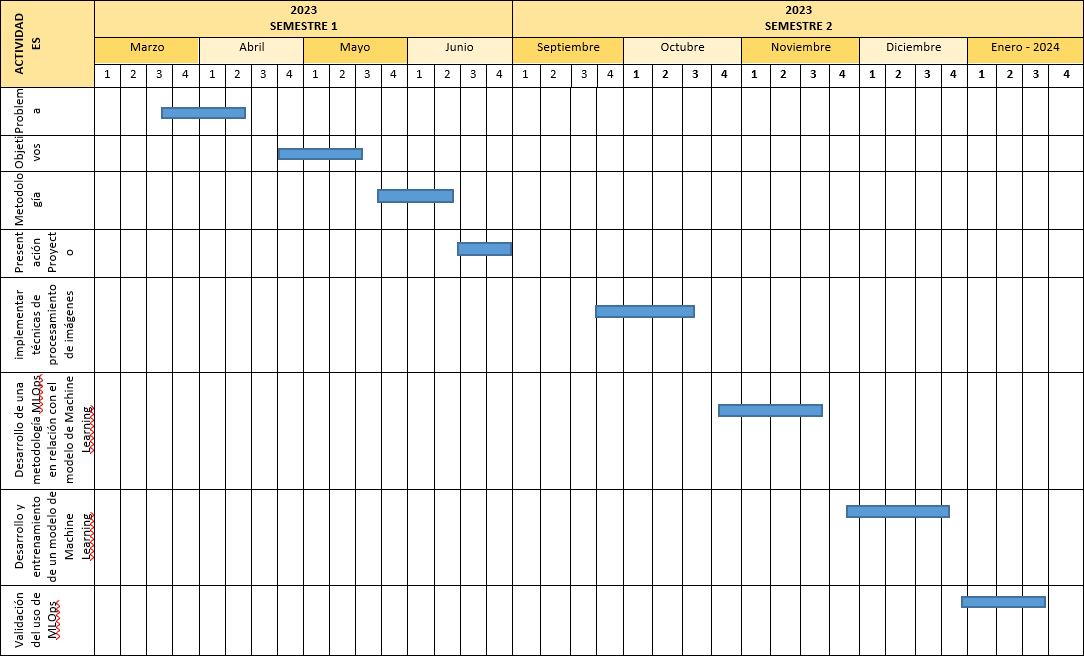
\includegraphics[width=1\textwidth]{img/cronogramaActividades.png}
\label{fig:figuraCronograma}
\end{figure}
%%\newpage

%% Resultados
\section{Resultados}

\subsection{Técnicas de procesamiento de imágenes para extraer características relevantes y mejorar la capacidad del modelo de Machine Learning en el reconocimiento y detección de las plagas Stenoma catenifer y heilipus lauri en el cultivo de aguacate Hass a partir de imágenes capturadas en campo.}

El preprocesamiento de las imágenes desempeña un papel crucial, donde se encuentra la eliminación de ruido, la corrección de la iluminación y el aumento de contraste permitiendo mejoras en la calidad de las imágenes, lo que facilita la observación, ubicación y detección de plagas. Además, la segmentación de la imagen, que implica dividirla en regiones de interés, permite aislar áreas afectadas por plagas, lo que simplifica dicho análisis.


\subsubsection{Exploración de datos}

El análisis exploratorio de datos partió de las 744 fotografía del cultivo de aguacate Hass con las cuales se reveló información valiosa sobre la distribución y características de las imágenes. Al examinar la distribución, se observa la variabilidad en la iluminación, color y perspectiva de las imágenes, indicando dos parámetros en la información, el primero corresponde a las imágenes que no presentan el impacto de las plagas (50 imágenes) y el segundo las imágenes que evidencian el proceso de la plaga en el cultivo (694 imágenes con plaga). Esto sugiere la necesidad de técnicas de pre-procesamiento para normalizar la información antes de cualquier análisis.

Por esta razón, se estableció dos carpetas de información donde una de ellas se consignan las fotografías que presentan las características de las plantas sana y en la otra carpeta se encuentran las fotografías que muestran las tipologías del impacto de las plagas.

\newpage

\begin{figure}[h]
\centering
\caption{Exploración de datos}
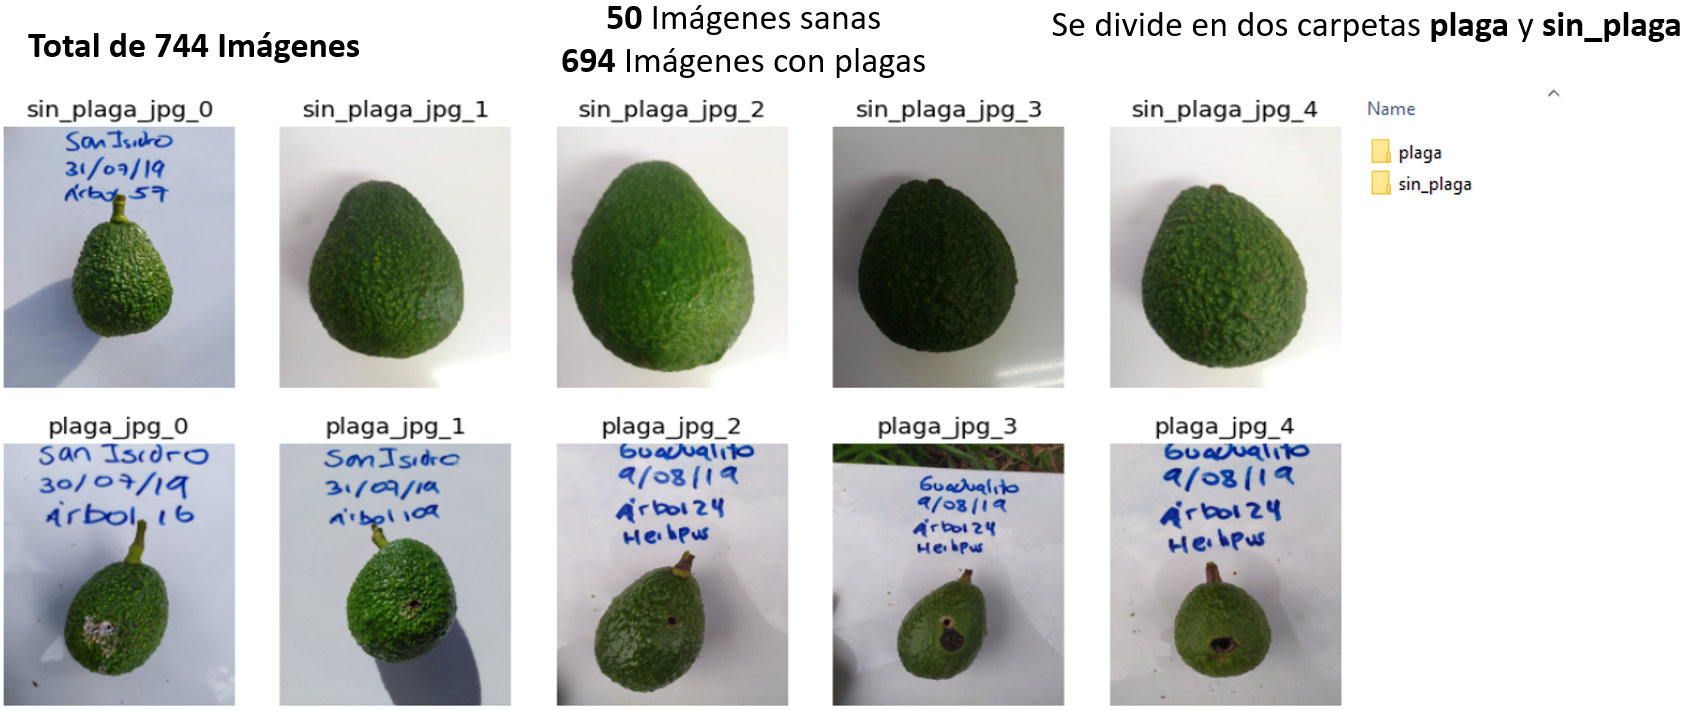
\includegraphics[width=1\textwidth]{resultados/expDatos.png}
\caption*{\footnotesize Fuente: Elaboración Propia}
\label{fig:figuraExpDatos}
\end{figure}


En este sentido, se desarrollaron algoritmos de extracción de características, como por ejemplo el histograma de colores, descriptores de texturas y las características basadas en formas, con las cuales se representa la información relevante de las imágenes dentro del cultivo, para que estas características se conviertan en entradas de reconocimiento en el modelo Machine Learning.

El siguiente código en Python está diseñado para la visualización de imágenes de cultivos de aguacate Hass, clasificadas en dos categorías: "Con Plaga" y "Sin Plaga". Este programa, destinado a ser ejecutado en un entorno de Jupyter Notebook, utiliza las bibliotecas Matplotlib y OpenCV. Su función principal es cargar y mostrar de manera detallada las dos tipologías definidas en las carpetas con imágenes de cada categoría, permitiendo una inspección visual clara de las características distintivas entre los cultivos afectados por plagas y aquellos que se consideran saludables.

\newpage

\begin{figure}[h]
\centering
\caption{código de extracción de características}
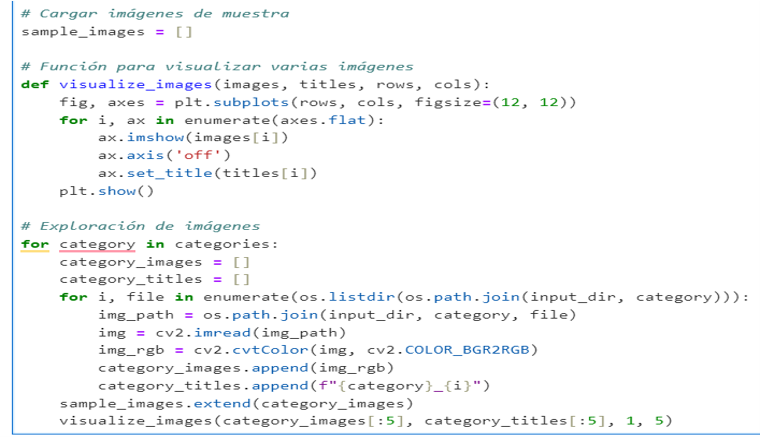
\includegraphics[width=1\textwidth]{resultados/codCaracteristicas.png}
\caption*{\footnotesize Fuente: Elaboración Propia}
\label{fig:figuraCodCaracteristicas}
\end{figure}

Este código estructurado simplifica la tarea de analizar visualmente las imágenes, proporcionando una representación clara de las dos clasificaciones, "Con Plaga" y "Sin Plaga", en el cultivo de aguacate Hass. Este código  generó una distribución de las imágenes por categoría para definir proporcionalmente cuántas imágenes se tenía de plaga y cuántas se tenían sin plaga.

Al realizar un análisis exploratorio de datos para comprender la distribución y características de las imágenes se puede señalar que, las imágenes sin plagas corresponden al 6,72\% y las imágenes con plagas el 93,28\% como se describe a continuación:

\newpage

\begin{figure}[h]
\centering
\caption{Distribución porcentual de las categorías de las imágenes}
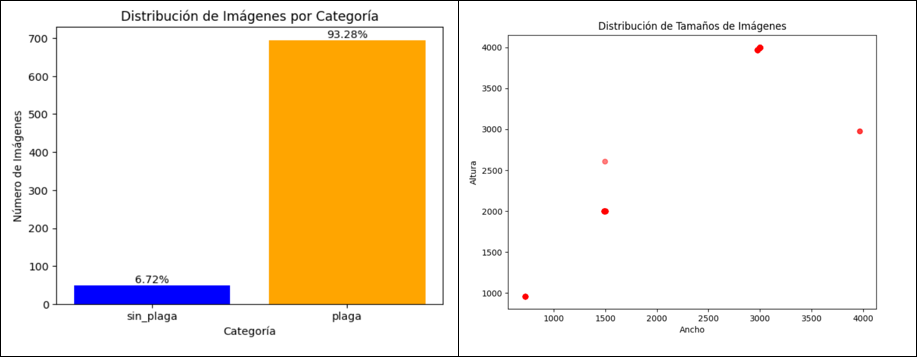
\includegraphics[width=1\textwidth]{resultados/distPorcentual.png}
\caption*{\footnotesize Fuente: Elaboración Propia}
\label{fig:figuraDistPorcentual}
\end{figure}

Se puede decir que las imágenes que generan mayor información corresponden a las que tienen plagas. Asimismo, la distribución de tamaño de imagen se observa que, identifican imágenes con un ancho de 4.000 píxeles por 3.000 píxeles de altura o por el contrario 3.000 de ancho por 4.000 de altura, donde se tomaron las fotografías tanto verticales como horizontales manteniendo esa rotación.

\newpage

\begin{figure}[h]
\centering
\caption{código imágenes por categoría y distribución de tamaño}
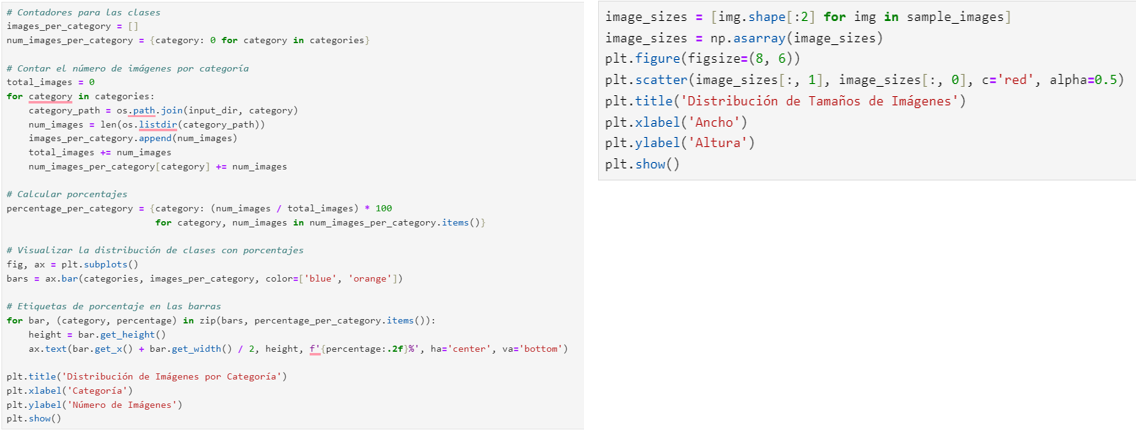
\includegraphics[width=1\textwidth]{resultados/codImagenes.png}
\caption*{\footnotesize Fuente: Elaboración Propia}
\label{fig:figuraCodImagenes}
\end{figure}

Este es el código correspondió para generar tanto la distribución de imágenes por categoría como la distribución por tamaños. 
Por otro lado, se generó un código para saber cómo está distribuido por cada alto y ancho de las imágenes. Como se puede ver en la imagen que el 87,6\% de las imágenes presentan una resolución de 4.000 píxeles por ancho y por el lado de las alturas más del 87,6\% tienen 3000 píxeles de alto.

\newpage

\begin{figure}[h]
\centering
\caption{Distribución alto y ancho de las imágenes}
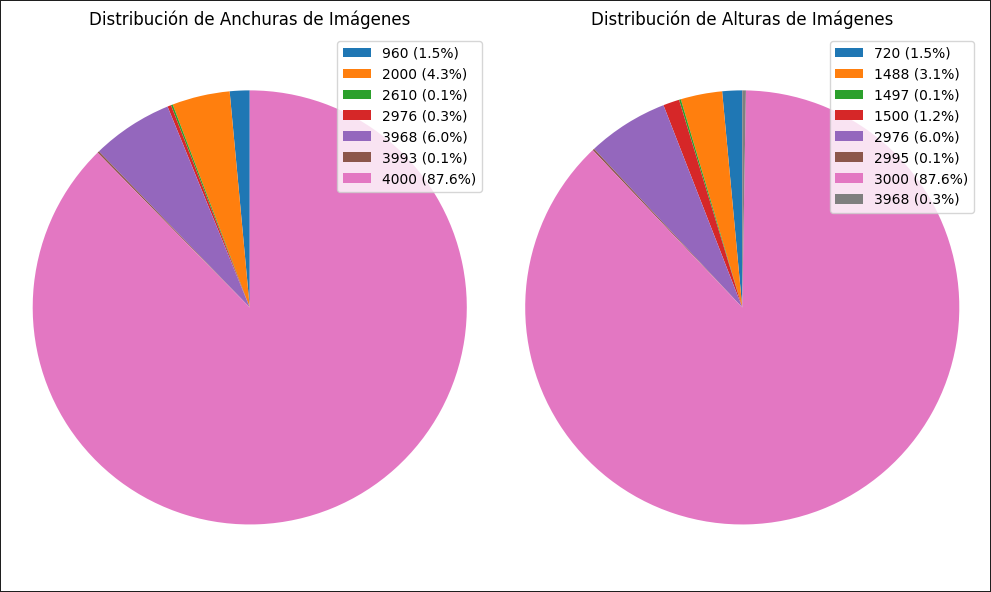
\includegraphics[width=1\textwidth]{resultados/distAlturas.png}
\caption*{\footnotesize Fuente: Elaboración Propia}
\label{fig:figuraDistAlturas}
\end{figure}

A continuación el código que me genera la distribución por alto y ancho de cada imagen

\newpage

\begin{figure}[h]
\centering
\caption{código de distribución alto y ancho}
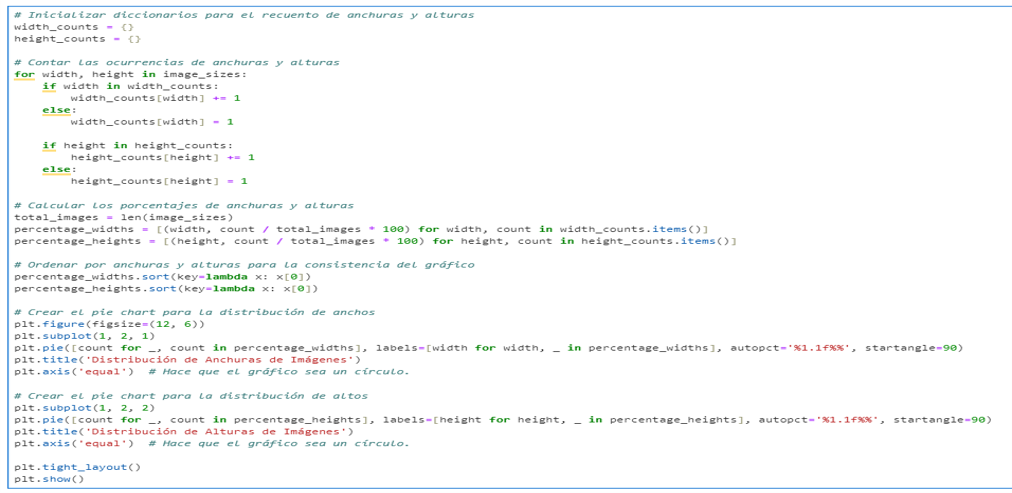
\includegraphics[width=1\textwidth]{resultados/codDistAlturas.png}
\caption*{\footnotesize Fuente: Elaboración Propia}
\label{fig:figuraCodDistAlturas}
\end{figure}

La exploración de datos, en una aplicación interactiva como Jupyter Notebook con Python, es relevante en el desarrollo de modelos de Machine Learning, ya que proporciona una comprensión de las características propias de los datos, facilita la toma de decisiones informadas sobre las imágenes que expresan información sobre si tienen plagas o no en el cultivo de aguacate Hass.

\subsubsection{Remoción de fondo de imagen}

Quitar el fondo de cada una de las imágenes dejando solo el aguacate, enfocándose solamente en las imágenes que muestra signos de plagas, es esencial en el análisis de las imágenes para la detección y monitoreo de enfermedades. Al aislar el aguacate de su entorno, se simplifica la tarea de identificación de posibles plagas y enfermedades, permitiendo una evaluación más precisa y eficiente.

\newpage

La extracción del fondo proporciona un contexto visual claro para el análisis de las lesiones y síntomas presentes en el aguacate Hass. Este enfoque mejora la capacidad de los algoritmos de visión para identificar patrones sutiles asociados con enfermedades específicas, ya que elimina distracciones no relevantes y optimiza la focalización en las características de interés.

\begin{figure}[h]
\centering
\caption{Proceso de remoción de fondo de las imágenes}
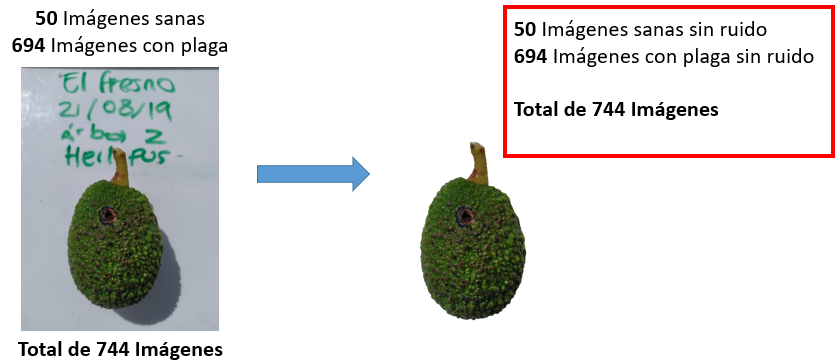
\includegraphics[width=1\textwidth]{resultados/remFondo.png}
\caption*{\footnotesize Fuente: Elaboración Propia}
\label{fig:figuraRemFondo}
\end{figure}

Todas las 744 imágenes presentaban un fondo que podría introducir ruido durante el análisis. Por lo tanto, se llevó a cabo un proceso para eliminar o separar las imágenes del fondo, dejándolas libres de ruido. El resultado final consiste en la preservación únicamente de la parte central de la imagen, que destaca el aguacate Hass, como se aprecia en la imagen anterior con el código implementado realiza la tarea de eliminar el fondo y retener solo la imagen del aguacate. 

Este proceso es crucial para mejorar la calidad del análisis de las imágenes, ya que reduce interferencias externas y resalta la región de interés. La efectividad de este código asegura que las imágenes estén listas para ser utilizadas en análisis más detallados y precisos relacionados con el aguacate y cualquier aspecto asociado, sin la interferencia de fondos indeseados.


\newpage

\begin{figure}[h]
\centering
\caption{código de eliminación de fondo}
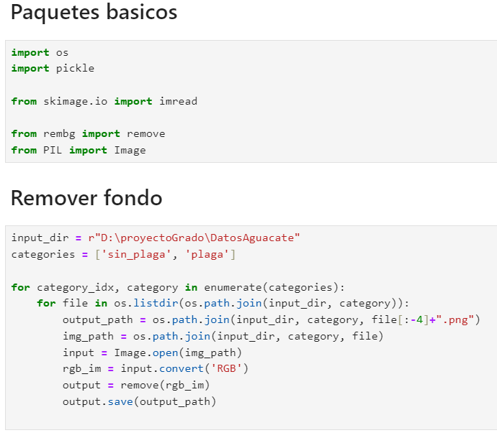
\includegraphics[width=1\textwidth]{resultados/codRemFondo.png}
\caption*{\footnotesize Fuente: Elaboración Propia}
\label{fig:figuraCodRemFondo}
\end{figure}

\subsubsection{Procesamiento de imágenes}

En el procesamiento de la segmentación de imágenes como se viene señalando en los anteriores momentos, permite resaltar la zona en donde se encuentra las caracteristicas propias de la plaga. El proceso tiene como fin facilitarle al algoritmo de Machine learning interpretar las imágenes. Este enfoque se integra en la fase de pre-procesamiento para resaltar la zona afectada por la plaga, simplificando la tarea del algoritmo y mejorando su capacidad de interpretación.

A cada una de estas 694 imágenes que presentan afectaciones de la plaga se trazó un polígono para saber en dónde estaba ubicada la plaga, este polígono genera unas coordenadas que luego van a ser interpretadas por uno de los algoritmos usados para el proyecto. 

\begin{figure}[h]
\centering
\caption{Proceso de segmentación de las imágenes}
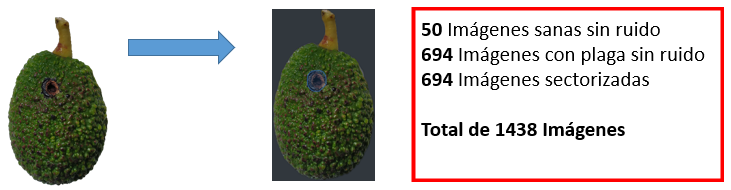
\includegraphics[width=1\textwidth]{resultados/proSeg.png}
\caption*{\footnotesize Fuente: Elaboración Propia}
\label{fig:figuraProSeg}
\end{figure}

Posteriormente se utilizó la aplicación DataTorch para hacer el trazado de los polígonos, en donde se coge una por una de las imágenes y se empieza a trazar cada una de las áreas en que se expresa la plaga, teniendo en cuenta que se hizo por cada una de las 694 imágenes dando un total de 1.438 imágenes, que incluye las imágenes sanas, las imágenes con plagas y las imágenes con los polígonos.

\begin{figure}[h]
\centering
\caption{Proceso de segmentación de las imágenes con DataTorch}
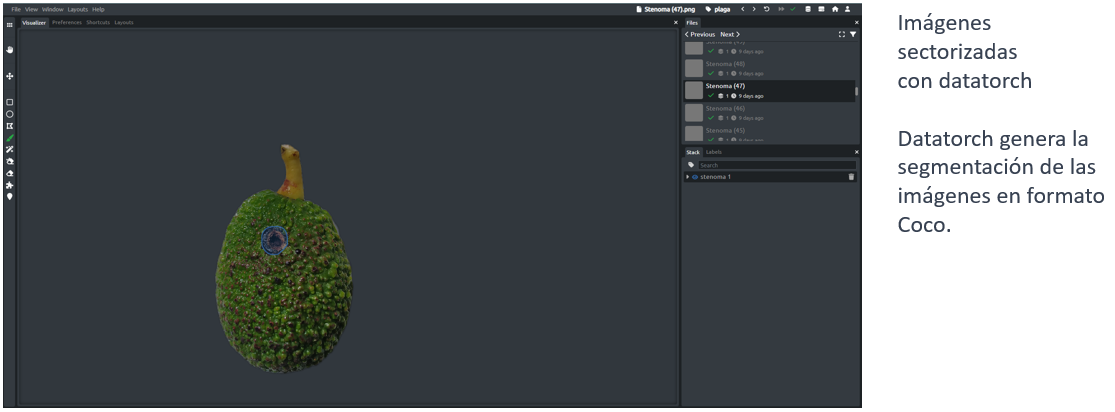
\includegraphics[width=1\textwidth]{resultados/proSeg2.png}
\caption*{\footnotesize Fuente: Elaboración Propia}
\label{fig:figuraProSegDatatorch}
\end{figure}


\newpage

\subsubsection{Conjunto de entrenamiento y prueba}

El proceso de entrenamiento en Machine Learning implica enseñar a un modelo a reconocer patrones y tomar decisiones basadas en datos. Para lograr esto, es necesario dividir el conjunto de datos normalmente en dos partes: la primera, conocida como conjunto de entrenamiento, se utiliza para alimentar al modelo con ejemplos que le permitan aprender patrones y relaciones entre variables. Esta fase busca ajustar los parámetros del modelo para que pueda generalizar y hacer predicciones precisas sobre datos no vistos anteriormente.

La segunda parte es el conjunto de validación, que actúa como una evaluación independiente del rendimiento del modelo. Al utilizar datos que el modelo no ha visto durante el entrenamiento, se puede evaluar su capacidad y prevenir problemas como el sobreajuste, donde el modelo memoriza los datos de entrenamiento en lugar de aprender patrones generales.

Dividir el conjunto de datos de las imágenes con plaga en conjuntos de entrenamiento y prueba como se describe a continuación:

\newpage

\begin{figure}[h]
\centering
\caption{Proceso de entrenamiento y validación}
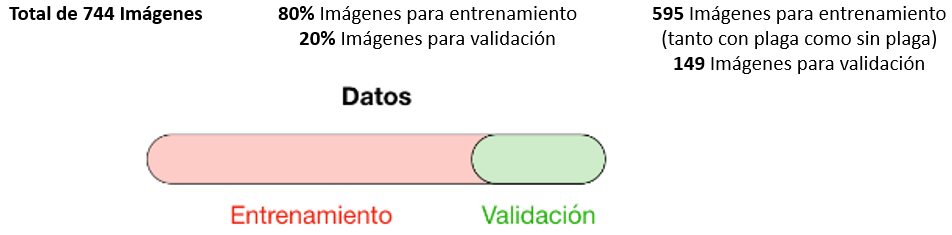
\includegraphics[width=1\textwidth]{resultados/proEntrenamiento.png}
\caption*{\footnotesize Fuente: Elaboración Propia}
\label{fig:figuraProEntrenamiento}
\end{figure}

Esta división en conjuntos de entrenamiento y validación es crucial para garantizar que el modelo pueda adaptarse a nuevos datos de manera efectiva, lo que mejora su capacidad predictiva y su utilidad en situaciones del mundo real. El proceso de la investigación es moderado, y puede manejar información de porcentajes de 80\% para entrenamiento y 20\% para validación. Cabe señalar que existen otros porcentajes como el 70 /30 refiriéndose a 70\% entrenamiento y 30\% de validación pero estos porcentajes son más útiles en conjuntos de datos más pequeños. 

Como para esta investigación se tiene un conjunto de datos moderado, es posible manejar un entrenamiento del de un 80/20; eso quiere decir que, del total de las imágenes 595 irán para el entrenamiento y 149 para validación, tanto la información con plaga como sin plaga, es decir se tiene toda la información conjunta.

\subsection{Metodología MLOps permitiendo la integración, automatización y monitoreo del modelo de Machine Learning diseñado para el reconocimiento y control de las plagas Stenoma catenifer y heilipus lauri en el cultivo de aguacate Hass}

\subsubsection{Selección de algoritmos}

Para el proyecto se deben seleccionar algoritmos de aprendizaje supervisado o no supervisado adecuados para el problema de detección de plagas. Se seleccionó el algoritmo de la regresión logística, que es un algoritmo de clasificación que ayuda a determinar la probabilidad de que una imagen tenga o no tenga un objeto en este caso una plaga. El proceso corresponde a clasificar de manera binaria, entre cero y uno, donde cero es que no tiene plaga y el objeto uno donde sí tiene plaga.

También, se seleccionó el algoritmo de Yolo V8, que sus siglas en ingles significan You Only Look Once. Este algoritmo emplea redes neuronales convolucionales, estamos hablando de Deep learning, para facilitar e interpretar las imágenes. Este enfoque se integra en la fase de pre-procesamiento que se encarga de resaltar la zona afectada por la plaga, simplificando la tarea del algoritmo de Machine Learning y mejorando su capacidad de interpretación.

Estas redes neuronales convolucionales pueden aprender patrones y características complejas, permitiendo la identificación precisa de plagas en imágenes agrícolas. Además, el Deep Learning facilita la interpretación de las imágenes al automatizar la extracción de características, eliminando la necesidad de diseñar manualmente algoritmos específicos.

\newpage

Para \cite{schmidhuber2015deep}, la capacidad del Deep Learning para adaptarse a patrones variados en imágenes, aprende automáticamente, agrupan gran cantidad de información, predicen comportamiento, los cuales contribuyen significativamente a mejorar la eficiencia y precisión en la detección de plagas. Su habilidad para generalizar a partir de conjuntos de datos grandes y diversos lo convierte en una herramienta poderosa para interpretar imágenes, proporcionando una base sólida para aplicaciones prácticas en la identificación y monitoreo de plagas, lo que en última instancia beneficia la gestión y la seguridad del proceso del cultivo de aguacate Hass.

\begin{figure}[h]
\centering
\caption{Acción del algoritmo Yolo V8}
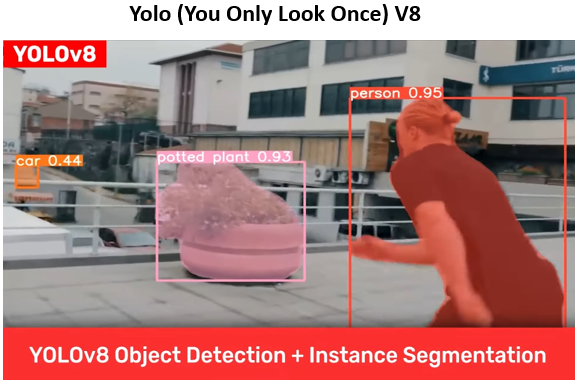
\includegraphics[width=1\textwidth]{resultados/yoloV8.png}
\caption*{\footnotesize Fuente: Elaboración Propia}
\label{fig:figuraYoloV8}
\end{figure}

\newpage

En la imagen se puede ver que se clasifica un objeto con un 95\% de probabilidad de que sea una persona, un 93\% de establecer el objeto como “planta” y el otro objeto que se ve corresponde a un 44\% que el objeto sea un “carro”. El algoritmo Yolo V8 incluso puede ser usado en video, permitiendo en este caso detectar objetos incluso en tiempo real.

La selección del algoritmo de regresión logística se da porque es uno de los estándares para trabajar clasificación de imágenes en la industria. Por otro lado, el algoritmo Yolo es un algoritmo de Deep learning, para detectar objetos en imágenes esto se hace para determinar con una probabilidad de qué objetos se tienen en una imagen o imágenes e incluso en videos, siendo posible clasificar cada objeto que se encuentra en una imagen o video.

\subsubsection{Pre-procesamiento adicional}

El pre-procesamiento adicional correspondió a normalizar el tamaño de las imágenes. Esta acción fue necesaria debido a que permite trabajar con modelos de aprendizaje automático, como la regresión logística y Yolo. Esto se hace con el fin de reducir la complejidad computacional porque al tener imágenes de una resolución muy alta se va a requerir más procesamiento de cómputo para empezar a analizar pixel por pixel; a su vez ayuda a tener una consistencia en la entrada del modelo, porque todos los valores o variables del entrenamiento tendrán las mismas dimensiones y así se evitan problemas relacionados con la variabilidad que se puedan tener en el tamaño de las imágenes.

También habrá una normalización del modelo con datos nuevos, es decir que, si es necesario ingresar datos nuevos al modelo, pasaran por esta normalización cada uno de los datos en una resolución determinada.

\newpage

Para la normalización de las dimensiones se definió un tamaño fijo de 640 píxeles, tanto de ancho como de alto, debido a que Yolo en su versión 8 maneja valores por defecto en esta resolución. Por esta razón, se mantuvo la misma resolución en los dos modelos seleccionados, tanto para el Yolo, que ya tiene por defecto este valor, como en la regresión logística. El siguiente código hace referencia a la normalización del tamaño de las imágenes, pero únicamente para el modelo de regresión logística, debido a que Yolo internamente hace esta normalización.

\begin{figure}[h]
\centering
\caption{normalización de las imágenes para la regresión logística}
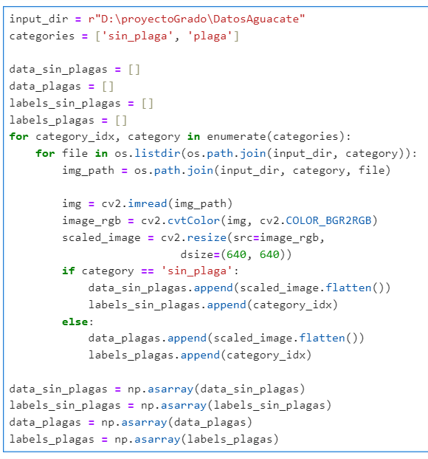
\includegraphics[width=0.7\textwidth]{resultados/normRegresion.png}
\caption*{\footnotesize Fuente: Elaboración Propia}
\label{fig:figuraNormRegresion}
\end{figure}

\newpage

\subsubsection{Implementación del modelo de regresión logística}

Para realizar la implementación del modelo de regresión logística, se realizó un balanceo de la información debido a la disparidad entre los datos con plagas (694), de los datos sanos (50). De allí que, se implementó un balanceo de información hacia abajo, es decir que la clase mayoritaria se tiene que igualar a su clase minoritaria para poder hacer comparaciones y hacer un entrenamiento más proporcional con la información.

\begin{figure}[h]
\centering
\caption{proceso de normalización de imágenes}
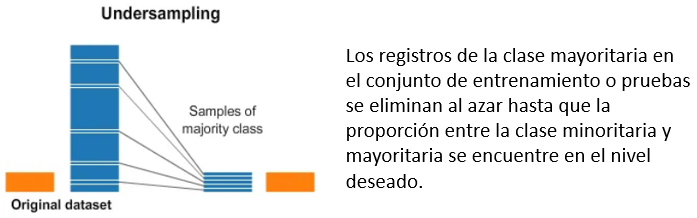
\includegraphics[width=0.8\textwidth]{resultados/proNormalizacion.png}
\caption*{\footnotesize Fuente: Elaboración Propia}
\label{fig:figuraProNormalizacion}
\end{figure}

Se realizó un submuestreo con validación cruzada (cross-validated subsampling). En este enfoque, se realiza repetidamente un submuestreo de la clase mayoritaria para equilibrar las clases y se evalúa el modelo en cada iteración utilizando la clase minoritaria. Luego, se promedian los resultados obtenidos en todas las iteraciones.

Este enfoque es especialmente útil cuando se trata con conjuntos de datos desequilibrados, donde una clase tiene muchas más datos (imágenes) que otra. Al realizar varias iteraciones y calcular promedios, se busca obtener una evaluación más robusta del rendimiento del modelo, ya que cada iteración puede tener una muestra diferente de la clase mayoritaria.

En el desarrollo de los scripts para implementar el modelo de regresión logística se realizan los siguientes pasos:

\newpage

\begin{enumerate}
    \item Se va a repetir el proceso de entrenamiento y evaluación 10 veces.
    \item Se realiza el balanceo de los datos en la clase mayoritaria (con plagas) sacando subconjuntos aleatorios de 50 imágenes del conjunto total (694).
    \item Se combinan los datos de 'sin plaga' y datos balanceados de 'plaga’ para tener un subconjunto de 100 imágenes totales 50 sin plaga y 50 con plaga.
    \item Se dividen los datos en conjuntos de entrenamiento y prueba en 80/20, es decir, 80 imágenes de entrenamiento y 20 imágenes para prueba.
    \item Se inicializa el modelo de regresión logística con la dependencia sklearn.
    \item Se pasa a entrenar el modelo con los subconjuntos de entrenamiento.
    \item Se realizan las predicciones en los subconjuntos de prueba.
    \item Se calcula la matriz de confusión y se almacena por cada subconjunto.
    \item Se calcula el promedio de las exactitudes (accuracy) obtenidas desde las matrices de confusión.
    \item Se calcula el promedio de las precisiones obtenidas desde las matrices de confusión.
    \item Se calcula el promedio de las sensibilidades (recall) obtenidas desde las matrices de confusión.
\end{enumerate}

\newpage

\begin{figure}[h]
\centering
\caption{código desarrollado para el modelo de regresión logística}
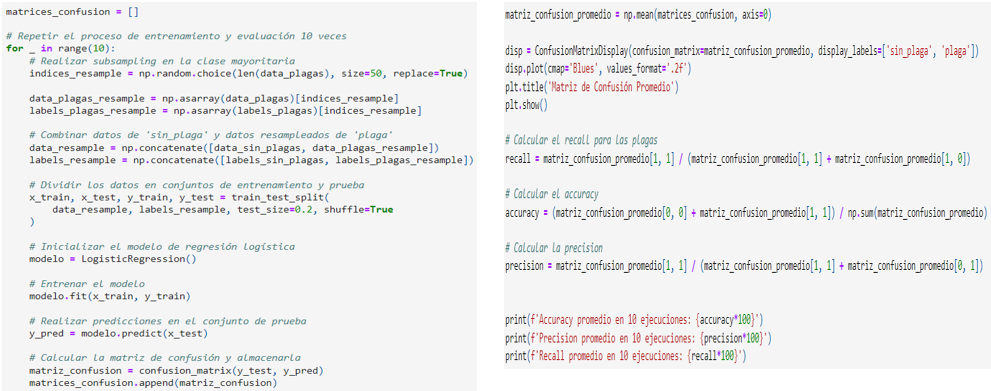
\includegraphics[width=1\textwidth]{resultados/codModelRegresion.png}
\caption*{\footnotesize Fuente: Elaboración Propia}
\label{fig:figuraCodModelRegresion}
\end{figure}

Para el desarrollo de los scripts que implementan el modelo Yolo V8 se realizaron los siguientes pasos:

\begin{enumerate}
    \item Se establece que se van a manejar por convención del modelo Yolo, dos particiones (entrenamiento – train y validación – validation) (ver figura \ref{fig:figuraConvencionYolo}).
    \item Se dividen los datos en las particiones de entrenamiento y prueba en 80\%/20\% de 744 imágenes, es decir, 595 imágenes de entrenamiento y 149 imágenes para prueba.
    \item Se realiza la transformación del formato Coco al formato Yolo para cada imagen  (ver figura \ref{fig:figuraCocoAYolo})\footnote{Se realiza la transformación del formato Coco para cada imagen al formato Yolo, porque en el objetivo uno la segmentación de imágenes se realizó con la herramienta DataTorch la cual utiliza el formato Coco para generar las anotaciones correspondientes en las imágenes, pero el algoritmo Yolo solo funciona con el formato Yolo.}.
    \item Se escribe en un archivo de texto la transformación del formato resultante.
    \item Se copia el archivo en la partición correspondiente (entrenamiento o prueba).
    \item Se importa la dependencia para trabajar con Yolo (ultralytics).
    \item Se establece el modelo a Yolo small \footnote{Yolo en su versión 8 salió en enero del año de 2023 y presenta diferentes modelos para diferentes tareas teniendo en cuenta las necesidades para detectar o segmentar información. Para esta investigación se manejó el modelo correspondiente a la detección de objetos. Para saber más sobre los diferentes tipos de modelos, se puede encontrar información detallada en el enlace \href{https://docs.ultralytics.com/es/models/yolov8/\#tareas-y-modos-compatibles}{tipos de modelos Yolo}. }. 
    \item Se establecen 10 épocas para correr el modelo.
    \item Se obtienen los resultados arrojados por el algoritmo (predicciones y sensibilidades - recall).
\end{enumerate}

El concepto de "épocas" se refiere a la cantidad de veces que todo el conjunto de datos se ha pasado hacia adelante y hacia atrás a través de la red neuronal durante el proceso de entrenamiento. Cada época representa una iteración completa a través de todo el conjunto de datos.
Manejar múltiples épocas durante el entrenamiento puede tener varios beneficios:

\textbf{Aprendizaje más Profundo:}

Las redes neuronales, incluidas las arquitecturas complejas como YOLO, pueden aprender patrones más profundos y sutiles a medida que se exponen repetidamente a los datos. Las épocas adicionales permiten que el modelo ajuste sus pesos en consecuencia y mejore su capacidad para generalizar a patrones más complejos.

\textbf{Mejora de la Generalización:}

El entrenamiento con más épocas puede ayudar a mejorar la capacidad del modelo para generalizar a datos no vistos. Esto es particularmente útil para evitar el sobreajuste, donde el modelo memoriza los datos de entrenamiento en lugar de aprender patrones, ubicaciones o lugares generales.

\textbf{Ajuste Fino de Parámetros:}

Las épocas adicionales permiten ajustar finamente los parámetros del modelo. A medida que el modelo ve los datos varias veces, puede hacer ajustes más precisos en los pesos para mejorar el rendimiento en el conjunto de entrenamiento.

\newpage

\textbf{Mejora de Métricas de Rendimiento:}

En muchos casos, las métricas de rendimiento (como precisión, recall, F1-score, etc.) pueden mejorar con un entrenamiento más prolongado. Las métricas estabilizan y pueden alcanzar su mejor rendimiento después de varias épocas.

Manejar 10 épocas podría ser mejor que manejar pocas épocas, esto puede depender de la complejidad del problema, del tamaño del conjunto de datos y de la arquitectura específica del modelo. Más épocas generalmente significan más oportunidades para que el modelo aprenda y mejore, siempre y cuando se evite el sobreajuste. Sin embargo, no siempre es necesario o beneficioso utilizar un gran número de épocas, ya que podría aumentar los costos computacionales sin proporcionar mejoras significativas en el rendimiento del modelo.

\begin{figure}[h]
\centering
\caption{código convención del modelo Yolo}
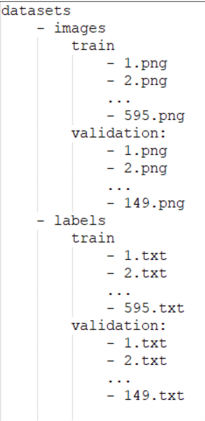
\includegraphics[width=1\textwidth]{resultados/convencionYolo.png}
\caption*{\footnotesize Fuente: Elaboración Propia}
\label{fig:figuraConvencionYolo}
\end{figure}

\newpage

\begin{figure}[h]
\centering
\caption{código transformación de formato Coco a formato Yolo}
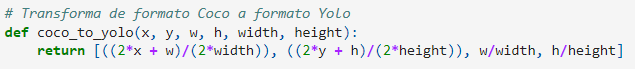
\includegraphics[width=1\textwidth]{resultados/cocoAYolo.png}
\caption*{\footnotesize Fuente: Elaboración Propia}
\label{fig:figuraCocoAYolo}
\end{figure}

Dentro del código anterior se especifica el cambio del formato Coco a Yolo partiendo de las categorías establecidas con la plaga y si no tiene plaga no se denota. Como se describe en el código se escribe las dimensiones de ancho y alto para las anotaciones, donde dice que para una imagen dentro del polígono se encuentra la plaga denotada en los cuatro lados expresados en cuatro valores (x, y, w, h) que son la coordenada X y Y en donde se ubica el extremo superior del polígono a marcar, como el ancho y alto en donde se encuentra la placa.

Estos parámetros de la cooredanada X y Y del polígono en formato Yolo, se posicionan en el centro de la imagen donde está ubicado el objeto, en este caso se mueve a su centro, y esto se hace con una fórmula matemática  como se observa en la siguiente imagen:


\begin{figure}[h]
\centering
\caption{proceso de cambio de Coco a Yolo}
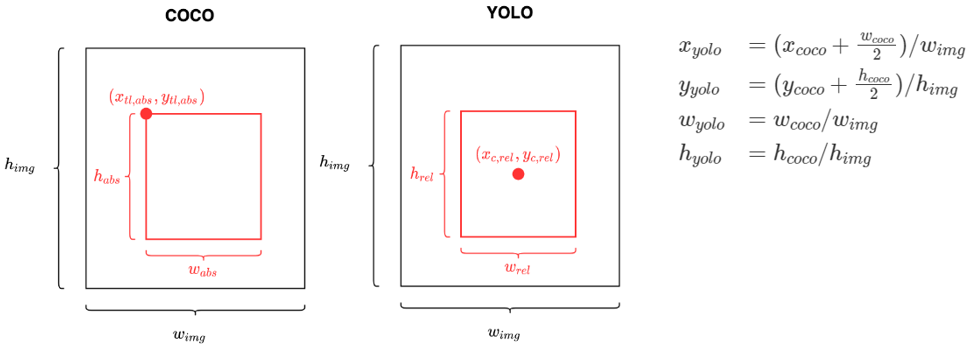
\includegraphics[width=1\textwidth]{resultados/camCocoAYolo.png}
\caption*{\footnotesize Fuente: Elaboración Propia}
\label{fig:figuraCamCocoAYolo}
\end{figure}

\newpage

Después de realizar la transformación, el procedimiento implica identificar y organizar la información (ver figura \ref{fig:figuraPoligonoCocoAYolo}) de la siguiente manera:
\begin{itemize}
    \item La primera columna especifica la clase a utilizar, en este caso, "plaga" \footnote{La acción matemática es descrita en \cite{rehman2022conversion} especificando los procedimientos para el cambio de Coco a Yolo.}. 
    \item La segunda y tercera columna indican las coordenadas del punto medio de un cuadro delimitador, correspondiente a la posición central del objeto a identificar, en este caso, la plaga. 
    \item La cuarta y quinta columna contienen las dimensiones del cuadro delimitador, representando respectivamente el ancho y alto del objeto en cuestión. Para clarificar. la cuarta columna representa el ancho, mientras que la quinta columna refleja el alto. Este proceso se aplica para facilitar la identificación y delimitación de la plaga.
\end{itemize}

\begin{figure}[h]
\centering
\caption{identificación del polígono cambio de Coco a Yolo}
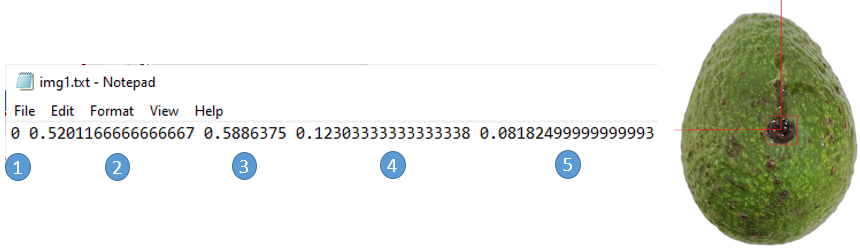
\includegraphics[width=1\textwidth]{resultados/poligonoCocoAYolo.png}
\caption*{\footnotesize Fuente: Elaboración Propia}
\label{fig:figuraPoligonoCocoAYolo}
\end{figure}

\newpage

Este proceso corresponde a la conversión del formato Coco a Yolo. En otras palabras, se especifica una clase, en este caso, "plaga" designada como cero. Los dos primeros valores indican las coordenadas del punto medio del cuadro que se va a delimitar, mientras que los dos valores restantes representan el alto y el ancho de la imagen en cuestión. Este código pertenece al modelo Yolo V8, donde se lleva a cabo la distribución de las imágenes en las dos particiones correspondientes de entrenamiento y validación.


\subsubsection{Implementación del modelo Yolo}

La siguiente imagen \ref{fig:figuraCodModelYolo} hace referencia a la implementación para el modelo Yolo. En donde:

\begin{itemize}
    \item Los puntos 1 y 2 hacen referencia al preprocesamiento que se le van a aplicar a las imágenes para el modelo Yolo.
    \item El punto 3 se observa que se carga el modelo en el código Yolo V8 en su versión small, definiendo las épocas, en este caso 10, las cuales van a procesar la información, teniendo en cuenta que entre más épocas mayor es el costo computacional para obtener un resultado. 
\end{itemize}

\newpage

\begin{figure}[h]
\centering
\caption{código desarrollado para el modelo Yolo V8}
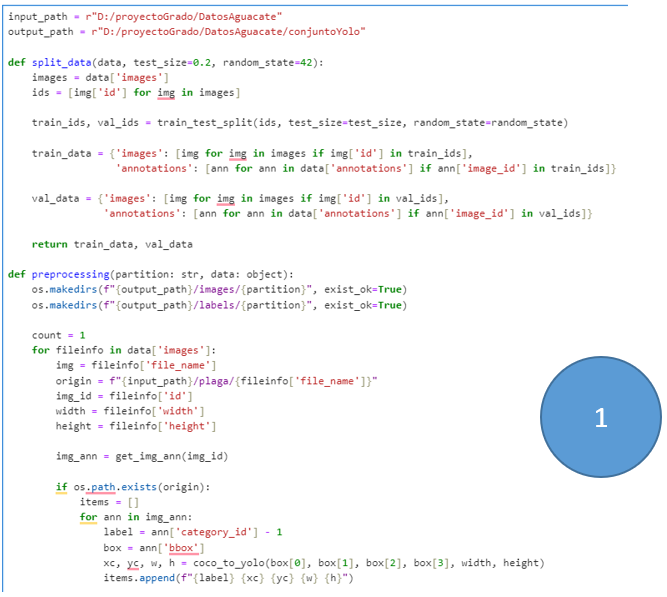
\includegraphics[width=0.4\textwidth]{resultados/codModelYoloP1.png}
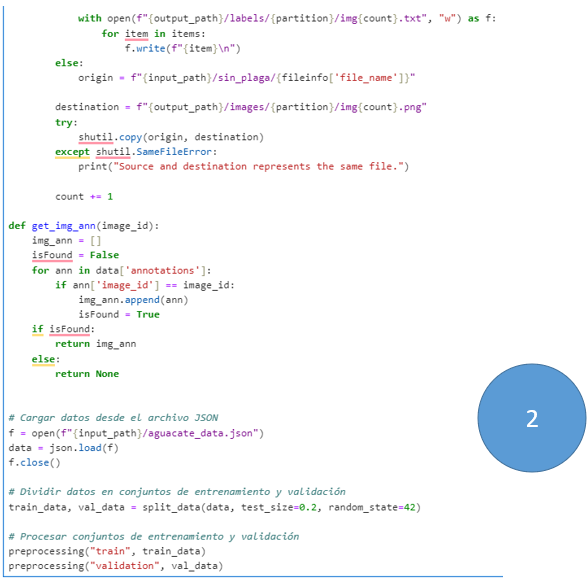
\includegraphics[width=0.4\textwidth]{resultados/codModelYoloP2.png}
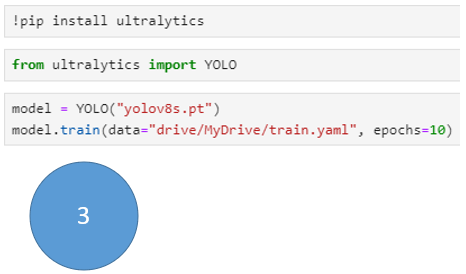
\includegraphics[width=0.4\textwidth]{resultados/codModelYoloP3.png}
\caption*{\footnotesize Fuente: Elaboración Propia}
\label{fig:figuraCodModelYolo}
\end{figure}

\subsubsection{Evaluación de los modelos}

Después de haber entrenado los modelos y pasar a predecir la información que se tenga del  conjunto de prueba, es decir identificar qué tanto aprendió y cuál fue el porcentaje de aprendizaje que se tuvo, para ambos casos se manejó una matriz de confusión donde se tienen cuatro lados: falso positivo, falso negativo, verdadero negativo, verdadero positivo (ver figura \ref{fig:figuraEvaModelos}).

\newpage

\begin{figure}[h]
\centering
\caption{Matriz de confusión para la evaluación de los modelos}
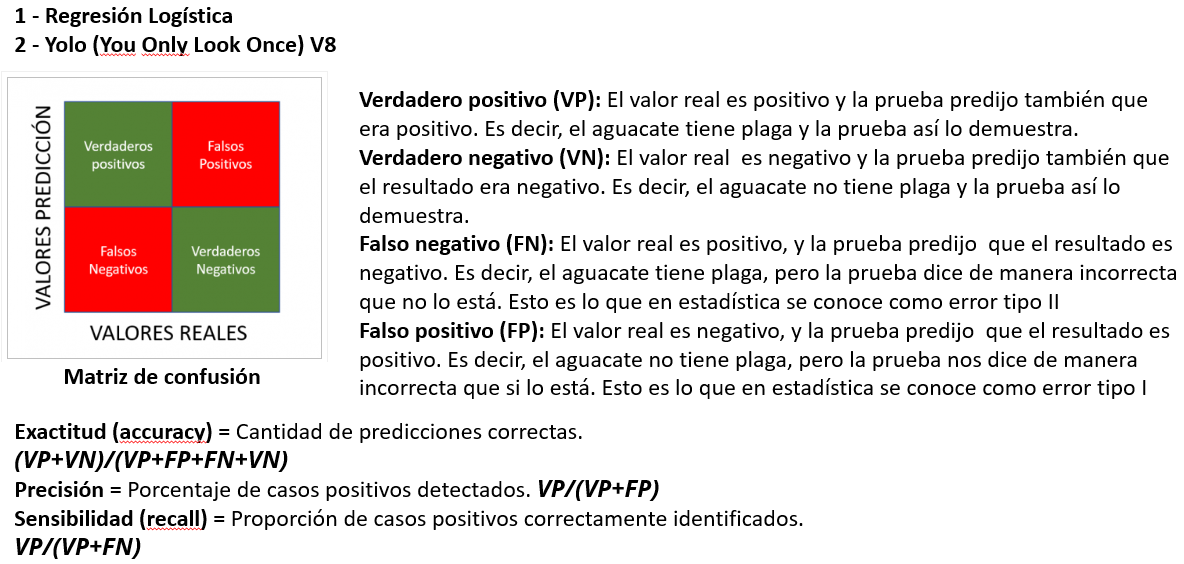
\includegraphics[width=1\textwidth]{resultados/evaModelos.png}
\caption*{\footnotesize Fuente: Elaboración Propia}
\label{fig:figuraEvaModelos}
\end{figure}

Una interpretación efectiva de la matriz de confusión en un modelo YOLO es esencial para entender cómo se comporta en términos de identificación y ubicación de objetos en las imágenes de entrada. Al analizar los elementos de la matriz, los científicos de datos pueden ajustar el modelo para mejorar su rendimiento y garantizar una detección precisa de objetos en diferentes escenarios y condiciones.

Para la regresión logística al tener 10 iteraciones se calculó el promedio de esas matrices de confusión, es decir que cada vez que se pasaba el modelo en este subconjunto de datos de 100 imágenes se estaba calculando una matriz de confusión, se van guardando cada una de esas matrices y al final lo que se hace es promediarlas, para tener los resultados de exactitud, precisión y sensibilidad como se describe en la imagen \ref{fig:figuraEjeProMatrizConfusion}.


\newpage

\begin{figure}[h]
\centering
\caption{resultado promedio de la matriz de confusión del modelo de regresión}
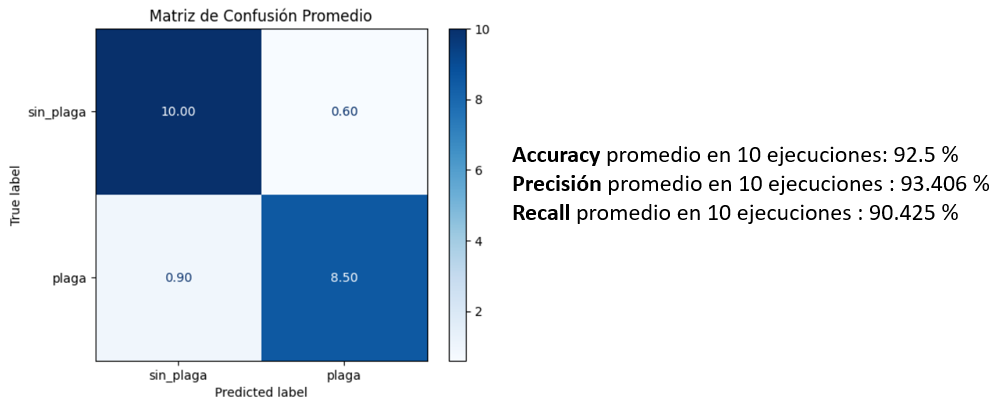
\includegraphics[width=1\textwidth]{resultados/ejeProMatrizConfusion.png}
\caption*{\footnotesize Fuente: Elaboración Propia}
\label{fig:figuraEjeProMatrizConfusion}
\end{figure}

El objetivo es determinar la cantidad de datos que estaban etiquetados como afectados por una plaga durante la prueba del modelo. En este escenario, se utiliza un subconjunto de 100 imágenes para llevar a cabo las pruebas, y se espera que dicho subconjunto represente un porcentaje específico del total correspondiente al 20\% para las pruehas.

Además, la parte de evaluación del modelo de regresión logística, después de haber hecho las iteraciones de la información para entrenar el modelo, en cada iteración se fue almacenando su matriz de confusión. Este proceso obtiene la matriz de confusión de cada uno de las iteraciones, las cuales se promedian y se obtienen el cálculo de la exactitud (accuracy), la precisión y la sensibilidad (recall), como se describe en el código de la imagen \ref{fig:figuraCodEvaModelRegresion}. 

Entonces eso quiere decir que cuando se habla de precisión se especifica la cantidad de casos positivos detectados, lo que significa que para este caso fueron realmente positivos detectados en un 93.4\%, una sensibilidad que corresponde a la proporción de los casos positivos correctamente identificados que fue de un 90.4\%. Para el caso de la exactitud se evidenció un 92.5\%, es decir la cantidad de predicciones correctas esta en este porcentaje, siendo un buen promedio de predicción para validar si una imagen tiene o no tiene plaga en un 92.5\%.



\begin{figure}[h]
\centering
\caption{código evaluación del modelo utilizando regresión logística en el conjunto de prueba.}
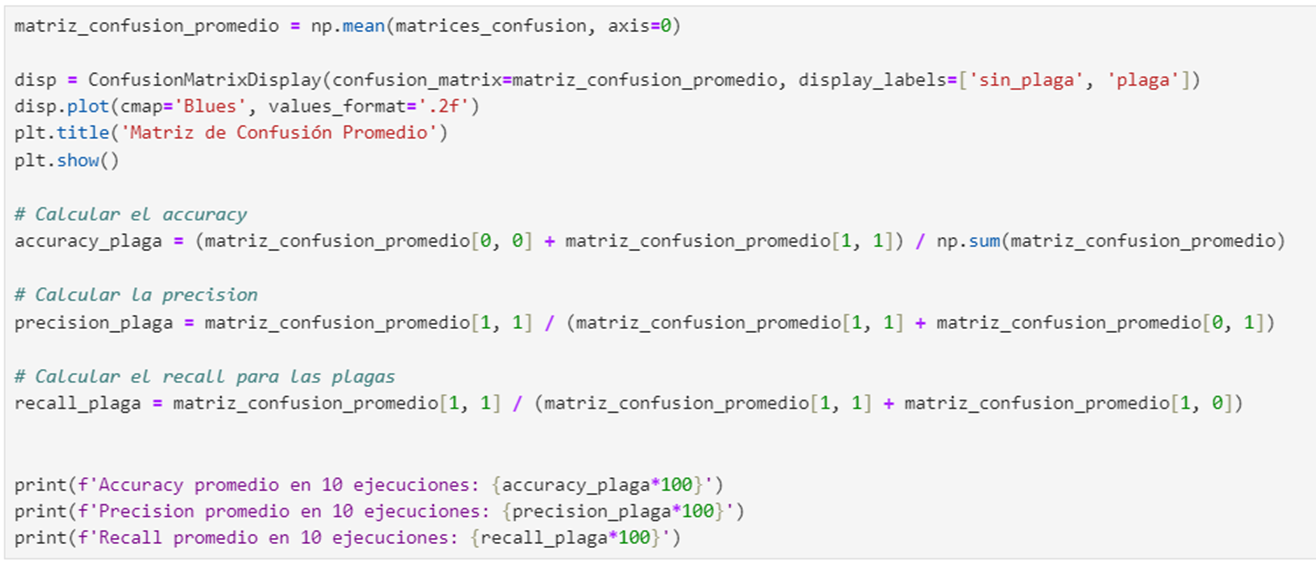
\includegraphics[width=1\textwidth]{resultados/codEvaModelRegresion.png}
\caption*{\footnotesize Fuente: Elaboración Propia}
\label{fig:figuraCodEvaModelRegresion}
\end{figure}

Si se volviera a ejecutar el programa, es posible que la información varíe ligeramente, pero en términos generales, los resultados que se presentan corresponden a la ejecución más reciente del algoritmo. Es importante destacar que las variaciones observadas en la exactitud, la precisión y la sensibilidad son mínimas. Estas fluctuaciones, aunque pueden existir cambios sutiles, la diferencia no es significativa.

En Yolo V8, ya no es necesario clasificar las imágenes que no contienen plagas. Ahora, el enfoque se centra únicamente en clasificar las imágenes que efectivamente presentan plagas. Cuando se procesa la información que carece de plagas, el algoritmo simplemente ignora o descarta dicha información, ya que el objetivo principal consiste en identificar si una imagen específica del conjunto de prueba contiene o no una subimagen, polígono o recuadro que pueda representar una plaga. En otras palabras, el propósito es determinar si dentro de la representación visual de un aguacate existe o no la presencia de una plaga. El enfoque se ha optimizado para dirigir la atención exclusivamente a las instancias relevantes, simplificando el proceso de clasificación y mejorando la eficiencia del modelo.


\newpage

\begin{figure}[h]
\centering
\caption{resultado del modelo Yolo V8}
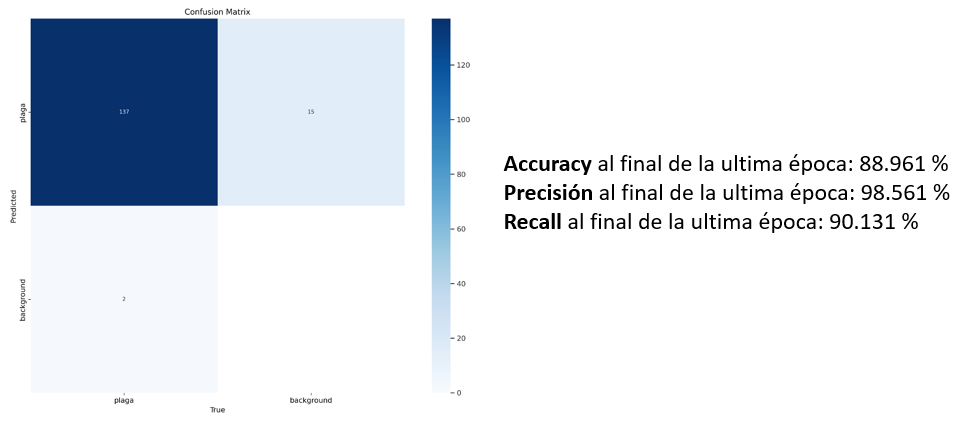
\includegraphics[width=1\textwidth]{resultados/ejeProMatrizConfusionYolo.png}
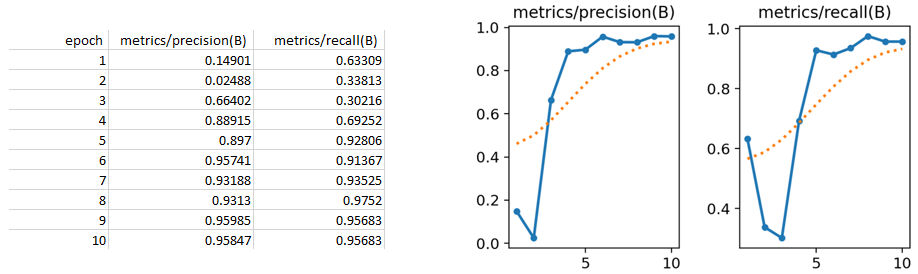
\includegraphics[width=1\textwidth]{resultados/resYolo.png}
\caption*{\footnotesize Fuente: Elaboración Propia}
\label{fig:figuraEjeProMatrizConfusion}
\end{figure}

Después de realizar la evaluación, observamos que la sensibilidad (recall) alcanzó un 90\%, indicando que el 90\% de los casos positivos fueron correctamente identificados respecto al total de imágenes. La precisión, que mide la proporción de casos positivos correctamente detectados entre las predicciones positivas, se situó en un sólido 98\%. Por otro lado, la exactitud (accuracy), que representa la cantidad general de predicciones correctas, se registró en un 88\%. Esto implica que, aunque se logró una alta precisión, hubo algunas predicciones incorrectas, especialmente en casos específicos evaluados por el modelo Yolo.


\newpage

Es importante destacar que la evaluación se llevó a cabo con imágenes que tenian y carecían de plagas, es decir, imágenes consideradas como "sanas". Además, es relevante señalar que la matriz de confusión se generó de manera automática, proporcionando una representación visual detallada de los resultados de la evaluación.

Yolo genera imágenes y proporciona métricas clave como precisión, recall y curvas de aprendizaje por época. Al analizar las estadísticas por época, se observa una progresión significativa en la precisión a lo largo del entrenamiento. En las primeras épocas, la precisión fue baja, alcanzando solo el 14.1\% en la primera y el 2\% en la segunda. Sin embargo, a partir de la tercera época, se observa un aumento marcado, llegando al 66\% en la época 6 y alcanzando un impresionante 95\% en la época 7. Las épocas 8, 9 y 10 mantienen rendimientos destacados, con la época 9 mostrando una precisión aún mayor que la 10 (ver figura \ref{fig:figuraEjeProMatrizConfusion}).

El análisis detallado revela que, a pesar de obtener altos valores de recall, la precisión disminuyó en la época 10, este análisis subraya la importancia de equilibrar la precisión y el recall al ajustar el número de épocas. La representación gráfica destaca cómo el modelo evoluciona en cada época, evidenciando mejoras notables a partir de la quinta época. La tabla complementa visualmente la información proporcionando valores precisos de precisión y recall para cada época. En retrospectiva, la decisión de detener el entrenamiento en la época 9 podría haber resultado en un rendimiento óptimo, ya que se logró una alta precisión sin comprometer significativamente el recall. Este análisis proporciona valiosas percepciones para optimizar futuros entrenamientos del modelo Yolo.

En los resultados proporcionados por el modelo, se presentan imágenes que fueron clasificadas como casos de plagas. Al analizar estas imágenes, es evidente que el modelo ha identificado correctamente la presencia de plagas, ya que estas son las mismas imágenes que proporcioné individualmente al algoritmo para su evaluación. En el conjunto de prueba generado, las representaciones visuales de plagas son claramente evidentes en las imágenes que se muestran en el lado derecho. Estas imágenes son el resultado de la aplicación del algoritmo, demostrando su capacidad para discernir y clasificar eficazmente las instancias de plagas en base a los patrones aprendidos durante el entrenamiento.

\newpage

\begin{figure}[h]
\centering
\caption{visualización de la evaluación realizada con Yolo V8}
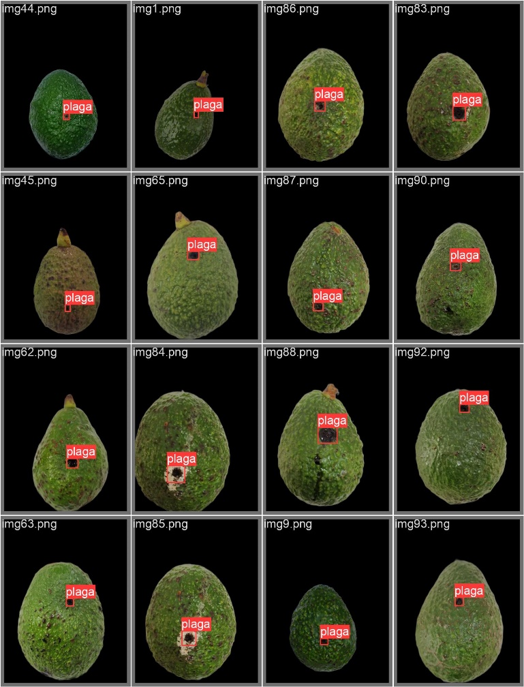
\includegraphics[width=1\textwidth]{resultados/visPruebasYolo.png}
\caption*{\footnotesize Fuente: Elaboración Propia}
\label{fig:figuraVisPruebasYolo}
\end{figure}

Este conjunto de resultados subraya la eficacia del modelo Yolo en la tarea específica de identificación de plagas, respaldando la calidad de las predicciones al compararlas con la evaluación visual que se realizó de manera automática. La capacidad del algoritmo para generalizar y reconocer patrones de plagas en nuevas imágenes es un indicativo positivo de su rendimiento y validez en aplicaciones prácticas relacionadas con la detección y clasificación de problemas específicos, como la presencia de plagas en cultivos.

Al evaluar el desempeño del algoritmo Yolo V8 en la validación de imágenes de plagas, se destaca la efectividad de la detección. En el conjunto de validación, el algoritmo demuestra su capacidad para identificar plagas en imágenes específicas sin conocer previamente la ubicación de los polígonos anotados. La separación del conjunto de datos en entrenamiento y prueba es esencial, y el conjunto de validación, con un 20\% de las imágenes, se utiliza para evaluar el rendimiento del modelo.

\newpage

Las imágenes seleccionadas para la validación no siguen un orden específico y son elegidas al azar por el algoritmo. Al analizar las imágenes detectadas, el algoritmo asigna porcentajes de confianza para cada región identificada como plaga, facilitando la interpretación de la certeza de las predicciones. Se observa que el algoritmo genera predicciones de plagas con confianza superior al 70\%.

La potencial aplicación práctica del modelo se ilustra al considerar su capacidad para clasificar imágenes en tiempo real, incluso mediante el análisis de videos. Esta capacidad permite no solo la detección de plagas, sino también la visualización gráfica instantánea de las áreas afectadas. La versatilidad del modelo Yolo V8 corresponde al poder aplicarse en situaciones dinámicas y en tiempo real.

\subsection{Modelo de Machine Learning utilizando técnicas apropiadas de preprocesamiento y selección de características, así como algoritmos de aprendizaje supervisado o no supervisado, para lograr una detección de las plagas Stenoma catenifer y heilipus lauri en el cultivo de aguacate Hass}

\subsubsection{Creación del flujo de trabajo con MLOps}

Dentro del un flujo de trabajo con MLOps que incluya la integración continua, entrega continua y monitoreo del modelo o los modelos normalmente siguiendo una fuente de información presentan una serie de niveles de madurez que permiten implementar la metodología de acuerdo con los avances u objetivos propios requeridos (ver tabla \ref{tab:tabFlujoTrabajo}).

\begin{longtable}{|p{2cm}|p{3cm}|p{5cm}|p{5cm}|}

\caption{Flujo de trabajo con MLOps}\\
    \hline
    \textbf{Nivel} & \textbf{Descripción} & \textbf{Características} & \textbf{Tecnología} \\
    \hline
    \endhead
        0 & Sin MLOps & \begin{itemize}\item Difícil gestionar el ciclo de vida completo del modelo de aprendizaje automático. \item Los equipos son dispares y las liberaciones son difíciles. \item La mayoría de los sistemas existen como "cajas negras", poca retroalimentación durante o después de la implementación.\end{itemize} & \begin{itemize}\item Construcciones e implementaciones manuales. \item Prueba manual de modelo y aplicación. \item Sin seguimiento centralizado del rendimiento del modelo. \item El entrenamiento del modelo es manual.\end{itemize} \\
        \hline
        1 & DevOps pero sin MLOps & \begin{itemize}\item Los despliegues son menos difíciles que el nivel 0, pero dependen del equipo de datos para cada modelo nuevo. \item Comentarios aún limitados sobre qué tan bien se desempeña un modelo en producción. \item Difícil rastrear/reproducir resultados.\end{itemize} & \begin{itemize}\item Construcciones automatizadas. \item Pruebas automatizadas para el código de la aplicación.\end{itemize} \\
        \hline
        2 & Entrenamiento automatizado & \begin{itemize}\item El ambiente de entrenamiento está totalmente gestionado y rastreable. \item Modelo fácil de reproducir. \item Los despliegues son manuales, pero de baja fricción.\end{itemize} & \begin{itemize}\item Entrenamiento de modelos automatizado. \item Seguimiento centralizado del rendimiento del entrenamiento del modelo. \item Gestión de modelos.\end{itemize} \\
        \hline
        3 & Implementación automatizada del modelo & \begin{itemize}\item Los despliegues son de baja fricción y automáticos. \item Trazabilidad completa desde la implementación hasta los datos originales. \item Todo el entorno gestionado: entrenamiento - prueba - producción\end{itemize} & \begin{itemize}\item Pruebas automatizadas para todo el código. \item Seguimiento centralizado del rendimiento del entrenamiento del modelo.\end{itemize} \\
        \hline
        4 & Operaciones automatizadas completas de MLOps & \begin{itemize}\item Sistema completo automatizado y fácilmente monitoreado. \item Los sistemas de producción están proporcionando información sobre cómo mejorar y, en algunos casos, mejorar automáticamente con nuevos modelos. \item Acercándose a un sistema sin tiempo de inactividad.\end{itemize} & \begin{itemize}\item Entrenamiento y pruebas de modelos automatizados. \item Métricas detalladas y centralizadas del modelo implementado.\end{itemize} \\
    \hline
    \caption*{\footnotesize Fuente: \cite{microsoft2023}}
    \label{tab:tabFlujoTrabajo}
\end{longtable}

\newpage

Como se puede observar en la tabla, en el nivel 0 para aplicar MLOps, nos encontramos con diversas características y tecnologías aplicables, pero predominan procesos manuales en varias etapas del modelo y su aplicación. Al avanzar al nivel 1, la atención se centra en la mejora del proceso, aquí, la generación de un nuevo modelo sigue siendo intensiva en términos de intervención del profesional ya que, rastrear y reproducir resultados se convierte en una tarea complicada. Dependiendo fuertemente del equipo de trabajo, el nivel 1 destaca la necesidad de mejorar la automatización en el ciclo de vida del modelo. \newline

Para el nivel 2 se marca un paso hacia la automatización del modelo, porque el ambiente de entrenamiento está completamente gestionado y se puede rastrear y reproducir fácilmente los resultados. Con el entrenamiento automatizado de modelos, se supera la dependencia manual del proceso y se avanza hacia una mayor eficiencia. Al llegar al nivel 3, se implementa la automatización del modelo, acompañado de pruebas automatizadas. La columna de tecnología resalta la importancia de la automatización de pruebas para todo el código, o al menos para partes críticas. Este nivel representa una mejora del ciclo de vida del modelo. \newline

Finalmente, en el nivel 4, se alcanza un estado avanzado de MLOps, tanto el entrenamiento como las pruebas ya que son completamente automatizados. Se incorporan métricas detalladas y descentralizadas del modelo implementado. Este nivel cumple plenamente con los principios de MLOps, marcando la culminación de un ciclo de vida de modelo altamente eficiente y gestionado. \citep{rivero2022, visengeriyeva2020}.

Para la implementación del modelo MLOps se encuentra detallada en un diagrama de flujo

\newpage

\begin{figure}[h]
\centering
\caption{Diagrama de flujo MLOps aplicado al proyecto}
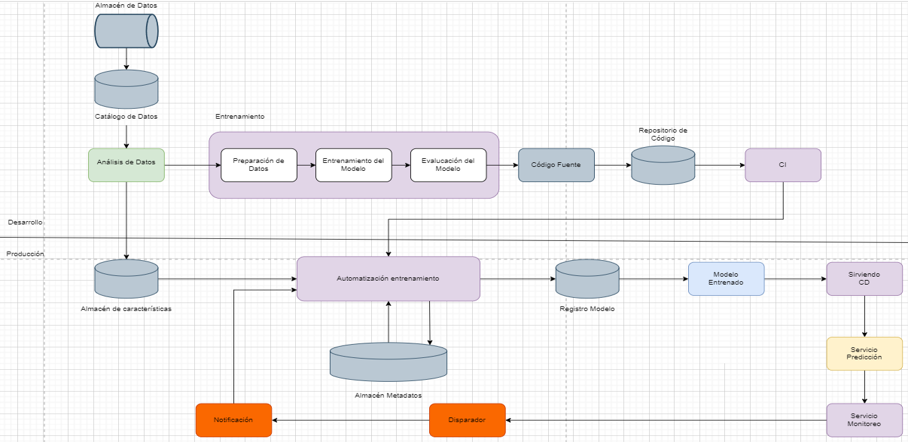
\includegraphics[width=1\textwidth]{resultados/flujoMLOps.png}
\caption*{\footnotesize Fuente: Elaboración Propia}
\label{fig:figuraFlujoMLOps}
\end{figure}

Se observa un proceso que se divide en dos etapas fundamentales: la etapa de desarrollo y la etapa de producción. En la fase de desarrollo, que generalmente se alinea con los objetivos uno y dos, se enfoca en el preprocesamiento de datos, abordando tareas como normalización, escalado de imágenes o redimensionamiento a dimensiones específicas. \newline

Durante esta etapa, se inicia la definición del entrenamiento y evaluación de datos. Con la implementación del MLOps, se introduce el versionado del código, permitiendo el control de cambios y la trazabilidad de la información. Un aspecto destacado es la iniciación del versionado de datos, donde se almacenan características específicas. En el contexto de un modelo de regresión logística, se determinan parámetros críticos como la cantidad de ciclos para el balanceo de datos, el tamaño de la muestra y el porcentaje asignado para las pruebas, cumpliendo con el previamente establecido 20\%. En la fase de producción se identifican los procesos de guardar la información esencial, como los modelos resultantes y sus respectivos desempeños, precisión y otros indicadores, todo centralizado en un sistema de registro de modelos. \newline

Continuando con el flujo del proceso, se registra la información del código fuente, es decir, la ubicación donde se crearon los códigos para la generación del modelo, siendo esta información cargada en una fuente de datos en línea. Este momento marca la viabilidad de realizar la integración continua, que se lleva a cabo mediante la misma herramienta de versionado de código, estableciendo así un flujo de trabajo continuo en el desarrollo del modelo. \newline

La fase de integración continua se realiza a través de la misma herramienta de repositorio de código que respalda el versionado del código. A continuación, se automatiza el proceso de entrenamiento del modelo, descrito en la fase de producción, que contribuye a una automatización progresiva. En este enfoque, el entrenamiento se configura automáticamente en intervalos regulares o después de ciertas tareas específicas, generando de manera continua registros de modelos en desarrollo. \newline

En otras palabras, cada vez que se inicia un entrenamiento, se registra un nuevo modelo, listo para su implementación posterior. Este modelo entrenado se despliega y se expone a través de una API, facilitando el acceso desde diversos dispositivos, ya sea una computadora o un teléfono celular. Además, se crea una aplicación web que permite a los usuarios cargar imágenes simples para realizar predicciones sobre la presencia o ausencia de plagas. \newline

El proceso se complementa con un servicio de monitoreo diseñado para supervisar, registrar y verificar la información de los distintos modelos. Este monitoreo también se utiliza para analizar el rendimiento de los modelos, y en caso de un bajo rendimiento según las métricas establecidas, se activa un mecanismo de notificación. \newline

\newpage

Cuando el sistema detecta un bajo rendimiento, se dispara una notificación, generalmente a través de correo electrónico, que se envía directamente a un científico de datos. Este profesional evalúa la situación y determina los procesos a seguir para modificar y mejorar el rendimiento del modelo. El ciclo de integración continua, entrenamiento automatizado y monitoreo proactivo contribuyen a mantener y mejorar constantemente la eficacia de los modelos en producción. \newline

Un proceso de entrenamiento de un modelo debe ser escalable, colaborativo y reproducible. Los principios, herramientas y técnicas que garantizan que la construcción de modelos sea escalable, colaborativo y reproducible se conoce como MLOps. El MLOps seria llevar un modelo de ML desde su etapa de desarrollo a la etapa de producción y que se encuentre disponible para un usuario final, y a su vez sea confiable y eficiente.

Dentro de las características del MLOps confiable y eficiente se encuentran:

\begin{itemize}
    \item Buenas prácticas para crear código (variables y funciones de métodos adecuados para que se entienda el código elaborado).
    \item Control de versiones (código, datos y modelos de ML).
    \item Pruebas automáticas (sobre el flujo del sistema de ML para evitar fallas en el modelo que es el usado por los usuarios finales).
    \item Reproducibilidad (ayuda a obtener y replicar los mismos resultados con los datos y modelos anteriores).
    \item Documentación (ayuda a entender como fue realizado el código).
    \item Monitoreo (verifica cambios que pasan con el tiempo al modelo).
\end{itemize}

\newpage

A partir de estas características y específicamente después de realizar varias iteraciones para ajustar la parametrización de los modelos, se busca determinar cuál es el modelo óptimo que será implementado en producción. Durante este proceso de búsqueda, se versiona cada uno de los modelos en consideración y se compara su rendimiento para identificar el más eficiente. Cabe señalar que, se llevan a cabo pruebas automáticas en todo el modelo, contribuyendo así a la detección y prevención de posibles fallos en el flujo del modelo para ponerlo en producción. \newline

Las pruebas se realizan al modelo, siempre y cuando este no sea demasiado complejo de reentrenar o validar. En particular, se destaca que es más factible y eficiente entrenar el modelo de regresión logística en comparación con modelos más exigentes computacionalmente, como el modelo Yolo V8. Incluso con el primero, es posible usar la CPU únicamente para obtener un resulto, en contraste, el segundo requiere de la CPU y GPU simultáneamente. \newline

En el contexto de la reproducibilidad, se refiere a la capacidad de tener los datos en un punto específico, lo que significa que se puede rastrear qué datos se utilizaron exactamente para entrenar un modelo en particular. La reproducibilidad es esencial para replicar resultados en diferentes momentos en el tiempo. Este proceso se ve facilitado mediante una documentación que ayuda a comprender las acciones realizadas, especialmente en relación con el código de la solución implementada. La documentación proporciona la transparencia necesaria para entender el enfoque adoptado y los resultados obtenidos en cada fase del proceso.

\newpage

\begin{longtable}{|p{3cm}|p{5cm}|p{6cm}|}
\caption{Flujo de trabajo con MLOps}\\
    \hline
    \textbf{Elementos} & \textbf{Características} & \textbf{Acciones} \\
    \hline
    \endhead
        Análisis de datos & El análisis de datos se refiere al proceso de inspeccionar, limpiar, transformar y modelar datos con el objetivo de descubrir información útil, llegar a conclusiones y respaldar la toma de decisiones. & Durante esta etapa, se aborda la tarea de comprender la naturaleza de los datos, especialmente en el contexto de la identificación de plagas. Se busca discernir la presencia o ausencia de plagas, examinando la estructura y características de los datos. Se destacan acciones específicas, como la identificación de dimensiones desiguales en los datos, donde algunas muestras presentan mayor cantidad de píxeles en el ancho que en la altura. Ante esta diversidad, se afronta el desafío de establecer uniformidad en las dimensiones, asegurando coherencia en el conjunto de datos. \\
        \hline
        Feature Store (almacén de funciones) & Se almacenan las transformaciones que se le han aplicado a los datos, para después entrenar los modelos. & En el modelo de la regresión logística se remueve el fondo de las imágenes y después se redimensionan a un valor indicado de 640 x 640 pixeles. \\
        \hline
        Versionado del código & En donde se guarda todo el código generado, y se sube a internet. & Facilitar una integración adecuada de la solución realizada para los modelos tanto de regresión logística como Yolo V8. \\
        \hline
        Integración continua & Se refiere a la práctica de fusionar y validar regularmente los cambios de código en un repositorio compartido. & Permitir que diferentes miembros de un equipo de trabajo, pueden realizar una integración correcta de los códigos que se van agregando a un repositorio. \\
        \hline
        Versionado del modelo & Permite cambiar entre modelos en tiempo real o monitorear diferentes modelos & Se verifica cómo se van comportando los modelos dependiendo a parámetros que se le vayan cambiando y determinar cuál entre ellos es el mejor y poder después de haberlo identificado colocarlo en producción.  \\
        \hline
        Registro de modelos & Una vez que se ha entrenado un modelo, se almacena en un sistema de registro de modelos junto con sus metadatos. & Selección de parámetros por modelo a registrar, como ciclos de entrenamiento y numero de imágenes a emplear para la regresión logística. Cada una de estos parámetros, junto con el modelo entrenado, es agregado de manera integral al registro del modelo. La práctica de agregar estos metadatos al registro del modelo se realiza de manera continua, generando así versiones sucesivas del modelo a medida que se lleva a cabo el proceso de validación. \\
        \hline
        Model serving & Desplegar el modelo para que pueda ser usado por los usuarios, por medio de API y/o aplicación. & Sea en un computador, en una tablet o en un celular, el acceso al modelo se facilita para cualquier usuario, ya sea un individuo común o incluso un científico de datos. Se desarrolla una API y una aplicación con la finalidad de que el usuario final, pueda observar el comportamiento del modelo. La API y la aplicación permite pasar datos de prueba o datos reales, permitiendo así la validación de la existencia o no de plagas en un aguacate Hass. \\
        \hline
        Monitoreo de modelos & Se deben monitorear los modelos, para detectar cambios en el desempeño o puesta en producción. Esto es debido a que los modelos en producción pueden degradarse con el tiempo por los cambios en los datos de entrada, fallas en el sistema o fallas al momento de la generación del modelo. & Se lleva a cabo una monitorización continua para identificar cualquier cambio que pueda surgir en el rendimiento de un modelo. Este cambio puede manifestarse a través de variaciones en el rendimiento comparándose con una métrica global, así como errores de los servicios. Estas discrepancias pueden originarse por posibles fallas en diversas etapas del proceso. \\
        \hline
        CI / CD & Garantizan que el código se fusione frecuentemente donde se realicen compilaciones y pruebas automatizadas en un repositorio central. & En el proceso de MLOps, implica no solo probar el código, sino los modelos resultantes y desplegar el modelo en una API y/o una aplicación para los usuarios finales. \\
        \hline
        Almacén de metadatos & El registro es fundamental para la reproducibilidad. Se pueden registrar todos los parámetros pasados a un modelo, como las métricas después de evaluarlo o registros del hardware usado. & Se permite el registro de información de los modelos, debido a que es parte esencial para la reproducibilidad. Esto implica la retención de información, específica para el modelo, como los parámetros y las iteraciones realizadas, así como la cantidad de datos empleados durante el proceso de entrenamiento de un modelo, entre otros. Este registro es para garantizar la capacidad de reproducir exactamente las condiciones bajo las cuales se desarrolló un modelo en particular. \\
        \hline
        Almacén de metadatos & El registro es fundamental para la reproducibilidad. Se pueden registrar todos los parámetros pasados a un modelo, como las métricas después de evaluarlo o registros del hardware usado. & Se permite el registro de información de los modelos, debido a que es parte esencial para la reproducibilidad. Esto implica la retención de información, específica para el modelo, como los parámetros y las iteraciones realizadas, así como la cantidad de datos empleados durante el proceso de entrenamiento de un modelo, entre otros. Este registro es para garantizar la capacidad de reproducir exactamente las condiciones bajo las cuales se desarrolló un modelo en particular. \\
    \hline
    \caption*{\footnotesize Fuente: Elaboración propia}
    \label{tab:tabCicloMlops}
\end{longtable}

Profundizando en el ciclo del MLOps, se retoma la referencia previa a la integración continua y despliegue continuo. Estas dos fases trabajan en conjunto para asegurar que el código se fusiona de manera regular y que las implementaciones son compiladas y automatizadas en un repositorio central. La integración continua se centra en fusionar el código con frecuencia, implementando compilaciones automatizadas que son almacenadas en un repositorio central.

\newpage

En cuanto al proceso, no se limita únicamente a probar el código; también implica evaluar los modelos resultantes. Este paso incluye el despliegue del modelo en una aplicación, permitiendo que los usuarios finales consuman los resultados. La entrega continua va más allá, implicando la implementación de cambios en el código en un entorno de pruebas o producción. Esta fase facilita despliegues rápidos para corregir fallos o implementar cambios en un modelo, posibilitando su incorporación en un entorno de producción.

\subsubsection{Las diferentes herramientas que implementan MLOps}

Entre las diversas herramientas disponibles para el MLOps, se pueden clasificar en dos categorías distintas: las sencillas y las complejas. Las herramientas sencillas son particularmente útiles para facilitar el despliegue local, es decir, en un mismo ordenador o un servidor local. Este enfoque es especialmente adecuado para pequeñas empresas o equipos pequeños de investigación, donde varios miembros de un equipo de trabajo pueden acceder desde diferentes computadoras de manera local. Estas herramientas sencillas representan el primer paso para llevar la solución a la fase de despliegue, especialmente en entornos de producción. \newline

Por otro lado, las herramientas complejas están diseñadas para gestionar mayores capacidades de cómputo. Estas pueden configurarse con capacidades específicas, e incluso el sistema puede autoajustarse según el tráfico y los requisitos de almacenamiento, incorporando la funcionalidad conocida como "On Demand", donde son capaces de autoescalar según las necesidades del momento. \newline

\newpage

Después de implementar las herramientas sencillas, se puede aprovechar lo creado para desplegar una aplicación. Esta aplicación, inicialmente desarrollada o creada localmente, puede integrarse con uno de los servicios en la nube más comunes y populares. Estos servicios en la nube, como AWS, Azure, GCP, son seleccionados debido a su amplia cuota de mercado y su uso generalizado en la actualidad. Esto permite llevar la aplicación creada localmente a aprovechar las capacidades y escalabilidad que ofrecen los servicios en la nube para su despliegue. \newline

La implementación de un monitoreo completo plantea ciertas consideraciones, especialmente cuando se considera la adopción de herramientas complejas. La complejidad de estas herramientas conlleva un aumento en los costos, ya que se aplican cargos por el conjunto completo de funcionalidades que ofrecen. En comparación, optar por el despliegue local y utilizar solo una fracción de estas herramientas resulta más económico. \newline

Además del aspecto financiero, es crucial tener en cuenta que el uso de herramientas complejas implica una curva de aprendizaje significativa. Se requiere una inversión de tiempo y esfuerzo para adquirir los conocimientos necesarios y comprender cómo manipular eficazmente todo el ciclo del MLOps (ver figura \ref{fig:figuraHerramientasMLOps}). Esta curva de aprendizaje elevada puede representar una desventaja, ya que impone una barrera para aquellos que buscan implementar estas herramientas de manera efectiva. \newline

Se han ido desarrollando muchas herramientas que se pueden utilizar para implementar la metodología de MLOps tanto de acceso libre (open source) o de pago, para usar localmente o desde internet. Y se deben escoger cada una con base a las necesidades del proyecto.

\newpage

\begin{figure}[h]
\centering
\caption{Herramientas que implementan ciclo completo de MLOps}
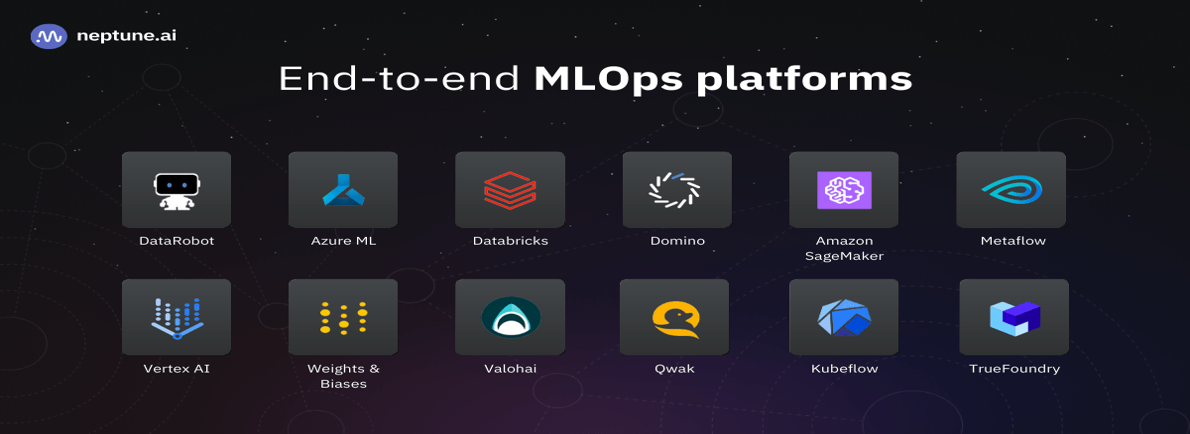
\includegraphics[width=1\textwidth]{resultados/herramientasMLOps.png}
\caption*{\footnotesize Fuente: \cite{neptune2024}}
\label{fig:figuraHerramientasMLOps}
\end{figure}

Dentro de las plataformas descritas en la imagen anterior se encuentra MetaFlow, esta plataforma en sí misma, es una herramienta gratuita, aunque algunas de sus funcionalidades pueden requerir pagos. Por ejemplo, el despliegue en internet podría estar sujeto a tarifas adicionales. Para completar todo el ciclo de vida del MLOps, es necesario considerar diversas herramientas, muchas de las cuales ofrecen características completas o parciales para gestionar eficazmente este ciclo. \newline

Para esta investigación se optó por seleccionar metodologías Open Source y se integraron  con Google Cloud Platform (GCP) para aprovechar características específicas. Aunque GCP es un servicio de pago, se ha utilizado la opción gratuita que proporciona un periodo de 90 días con fines educativos. Antes de que expire este período, es necesario cerrar la cuenta para evitar cargos adicionales. \newline

Como se viene mencionando, cada etapa del ciclo de vida del MLOps se cumple, total o parcialmente, mediante el uso de herramientas específicas (ver figura \ref{fig:figuraHerramientasAlmaAuto}, figura \ref{fig:figuraHerramientasAnaRepo}, figura \ref{fig:figuraHerramientasRegModDatos} e figura \ref{fig:figuraHerramientasDespApiApp}). Este enfoque garantiza una implementación efectiva y personalizada del ciclo de vida del MLOps, adaptándolo a las necesidades y requisitos específicos del proyecto.

\newpage

\begin{figure}[h]
\centering
\caption{Herramientas para almacenamiento y automatización de procesos}
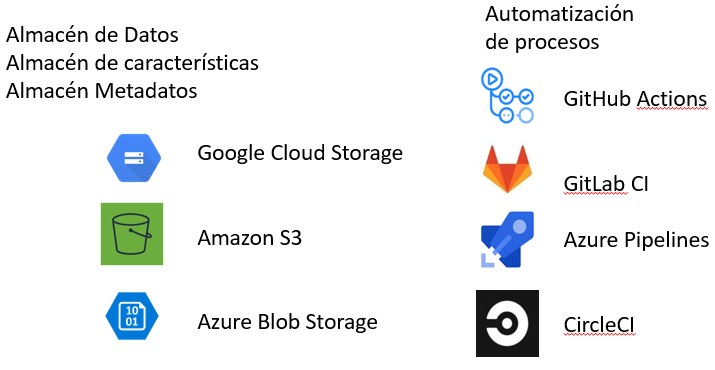
\includegraphics[width=1\textwidth]{resultados/herramientasAlmaAuto.png}
\caption*{\footnotesize Fuente: Elaboración propia}
\label{fig:figuraHerramientasAlmaAuto}
\end{figure}

Para esta implementación de MLOps se utilizó Jupyter, como se viene describiendo desde el objetivo 1. En cuanto al repositorio de código es en GitHub, que es una plataforma líder en el desarrollo colaborativo de software que proporciona servicios de alojamiento de repositorios Git, permitiendo a los miembros de un equipo trabajar juntos en proyectos, gestionar versiones de código y facilitar la colaboración distribuida.

\newpage

\begin{figure}[h]
\centering
\caption{Herramientas de análisis de datos y repositorio de código}
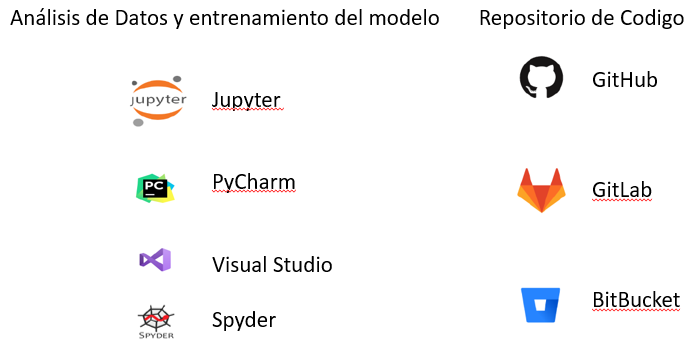
\includegraphics[width=1\textwidth]{resultados/herramientasAnaRepo.png}
\caption*{\footnotesize Fuente: Elaboración propia}
\label{fig:figuraHerramientasAnaRepo}
\end{figure}

\newpage

\begin{figure}[h]
\centering
\caption{Herramientas de registro de modelo, versionado del modelo y versionado de datos}
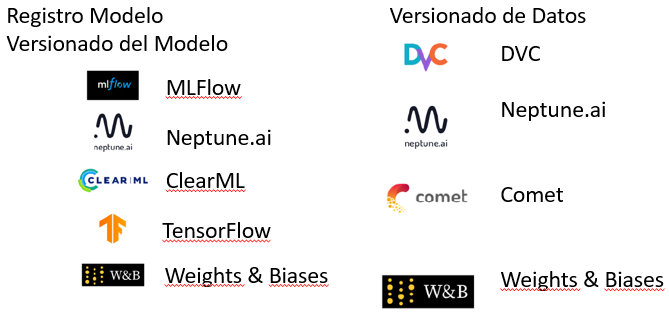
\includegraphics[width=0.7\textwidth]{resultados/herramientasRegModDatos.png}
\caption*{\footnotesize Fuente: Elaboración propia}
\label{fig:figuraHerramientasRegModDatos}
\end{figure}

\begin{figure}[h]
\centering
\caption{Herramientas para Construcción de API y Construcción de aplicación Web}
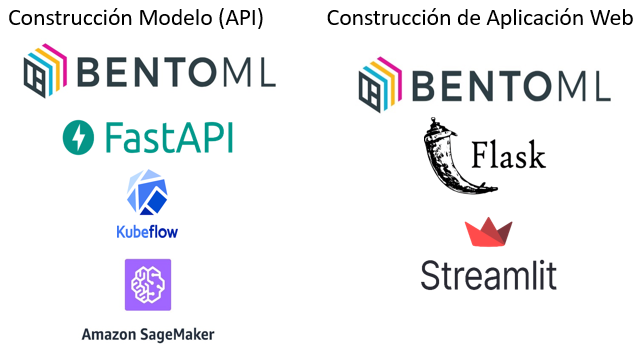
\includegraphics[width=0.6\textwidth]{resultados/herramientasDespApiApp.png}
\caption*{\footnotesize Fuente: Elaboración propia}
\label{fig:figuraHerramientasDespApiApp}
\end{figure}

\newpage

\begin{figure}[h]
\centering
\caption{Herramientas de Feature Store y Monitoreo del Modelo}
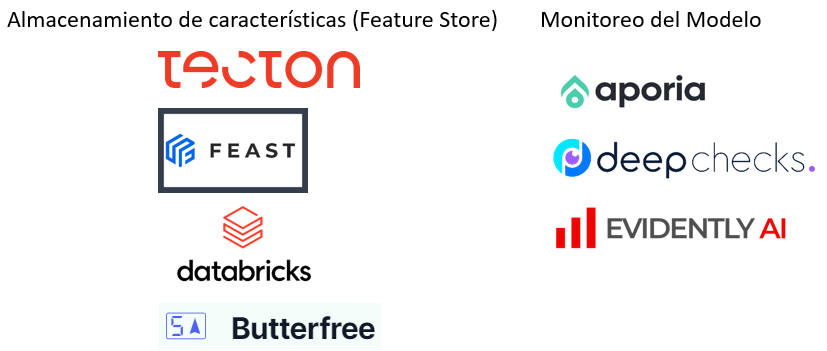
\includegraphics[width=0.9\textwidth]{resultados/herramientasFeaMon.png}
\caption*{\footnotesize Fuente: Elaboración propia}
\label{fig:figuraHerramientasFeaMon}
\end{figure}

\begin{figure}[h]
\centering
\caption{Herramientas utilizadas en el proyecto de MLOps para plagas en aguacate Hass}
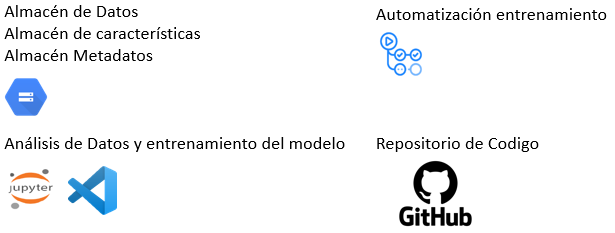
\includegraphics[width=0.7\textwidth]{resultados/herramientasAlmAutoAnaRep.png}
\caption*{\footnotesize Fuente: Elaboración propia}
\label{fig:figuraHerramientasAlmAutoAnaRep}
\end{figure}

\newpage

Las herramientas seleccionadas, como se mencionó una de ellas es Google Cloud Storage, elegida por su acceso gratuito durante 90 días, lo que permite manipular eficazmente este almacenamiento. Además, Google Cloud ofrece un crédito de alrededor de \$300 para utilizar diversas funciones de Google, lo cual resulta beneficioso para el análisis de datos. \newline

Otra herramienta clave es Visual Studio Code, que desempeñó un papel esencial en las transformaciones mencionadas. Fue especialmente útil para la transformación de los cuadernos de Jupyter a Python, proporcionando una interfaz intuitiva para manipular el código directamente en formato Python. Esto facilitó la gestión del código en un repositorio utilizando Git, donde se lleva a cabo el versionado de todas las partes del código y todo lo realizado en el desarrollo.

\newpage

\begin{figure}[h]
\centering
\caption{Herramientas utilizadas en el proyecto de MLOps para plagas en aguacate Hass}
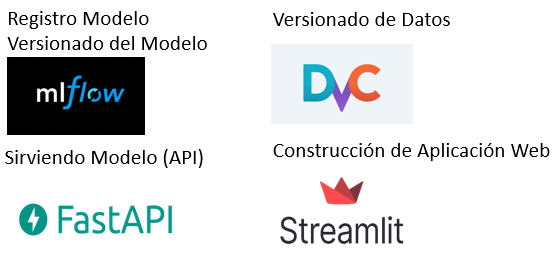
\includegraphics[width=0.7\textwidth]{resultados/herramientasRegVerCons.png}
\caption*{\footnotesize Fuente: Elaboración propia}
\label{fig:figuraHerramientasRegVerCons}
\end{figure}

Para el registro de modelos, se optó por MLFlow, una herramienta elegida por su eficacia en la gestión de versiones de modelos. En el ámbito del versionado de datos, se seleccionó la herramienta DVC, que facilita el almacenamiento de los datos por versiones. Para la construcción de aplicaciones web, se utilizó Streamlit. Para la implementación de la API, tanto local como remotamente, se empleó FastAPI. Es importante señalar que esta parte del proyecto, aunque extensa, es una extensión de la actividad 2 del objetivo tres, que implica la identificación de las herramientas empleadas para desarrollar la metodología MLOps en el proyecto.

\newpage

\begin{figure}[h]
\centering
\caption{Herramientas utilizadas en el proyecto de MLOps para plagas en aguacate Hass}

\includegraphics[width=0.7\textwidth]{resultados/herramientasMonAlmInt.png}
\caption*{\footnotesize Fuente: Elaboración propia}
\label{fig:figuraHerramientasMonAlmInt}
\end{figure}

En lo que respecta al monitoreo del modelo, se eligió realizar pruebas con Pytest, una dependencia de Python que evalúa el código y ejecuta pruebas. Este proceso de evaluación se lleva a cabo de manera programada a diario a las 4 de la mañana utilizando GitHub Actions, una herramienta de automatización de procesos. \newline

La elección del horario específico, las 4 de la mañana, se estableció para automatizar la ejecución de tareas en un momento menos propenso a la manipulación activa de modelos, especialmente por parte de los científicos de datos. No obstante, este horario podría ajustarse según necesidades y criterios específicos. \newline

En cuanto al almacenamiento de características, se utilizó Google Cloud Storage, empleando sus capacidades para almacenar las transformaciones aplicadas a las imágenes en el modelo de regresión logística. Cabe mencionar que, aunque se optó por este modelo para implementar la metodología MLOps debido a su menor consumo de recursos computacionales y tiempos de respuesta más rápidos en comparación con el modelo Yolo, esta metodología también se podría adaptar para Yolo según los requisitos específicos del modelo. \newline

Estas herramientas, cuidadosamente seleccionadas, ofrecieron una solución integral que abarcó desde el almacenamiento y análisis de datos hasta la gestión efectiva del código, de los datos, de los modelos y sus versiones, contribuyendo así al éxito del proyecto en el ámbito de la ingeniería de software.

\newpage

\subsubsection{Integración con herramientas MLOps}

Después de haber identificado las herramientas utilizadas para implementar MLOps. La sección se centra en el uso de estas herramientas y destaca el código disponible en un enlace proporcionado, organizado en una estructura específica de carpetas basada en una plantilla de ciencia de datos de cookiecutter\footnote{La plantilla se encuentra en el siguiente enlace de acceso público en GitHub \href{https://github.com/khuyentran1401/data-science-template/tree/dvc-pip}{aquí}.}, la cual es una dependencia de Python. El enlace a continuación proporciona acceso al código completo del proyecto, organizado de manera estructurada en carpetas con GitHub\footnote{Las carpetas y el código se encuentran en el siguiente enlace de acceso público en GitHub \href{https://github.com/juferoto/mlops_project}{aquí}.}.

\begin{figure}[h]
\centering
\caption{Estructura de las carpetas para el proyecto}
\includegraphics[width=1\textwidth]{resultados/estructuraCarpetas.png}
\caption*{\footnotesize Fuente: Elaboración propia}
\label{fig:figuraEstructuraCarpetas}
\end{figure}

La estructura de carpetas utilizada es esencial para comprender la lógica detrás de la implementación. Uno de los componentes de esta estructura es el "workflows", que almacena los archivos con extensiones Yaml y actúa como la base de las tareas automatizadas. Este punto será abordado de manera más detallada en el objetivo 4. Este enfoque en la organización y el propósito de las carpetas proporciona una visión clara de la implementación subyacente.

\newpage

Para realizar la ejecución local y obtener la estructura completa de carpetas desde el enlace proporcionado, se sigue un proceso que implica la clonación del repositorio desde GitHub. Una vez obtenida la información localmente, el código disponible puede ejecutarse para aquellos que lo necesiten. Todas las dependencias necesarias para el funcionamiento sin problemas del proyecto localmente están detalladas a continuación:


\begin{figure}[h]
\centering
\caption{Dependencias para trabajar con el proyecto localmente}
\includegraphics[width=0.5\textwidth]{resultados/dependenciasLocal.png}
\caption*{\footnotesize Fuente: Elaboración propia}
\label{fig:figuraDependenciasLocal}
\end{figure}

\newpage

Las dependencias del proyecto para trabajar de forma local se encuentran en la raíz del proyecto, en un archivo llamado dev-requirements.txt. Para instalar las diferentes dependencias seria con el comando: 
\begin{verbatim}
pip install -r dev-requirements.txt
\end{verbatim}

Cuando se clona el proyecto, se obtienen todos los archivos y carpetas en la ubicación local deseada. Una vez completada la clonación, se puede acceder a la estructura completa del proyecto. Este proyecto ha sido diseñado considerando todas las dependencias necesarias para su ejecución. \newline

En cuanto a la estructura de carpetas, se destaca la carpeta "models", que desempeña un papel crucial en el almacenamiento del modelo entrenado. En este contexto, el modelo de regresión logística, se almacena en formato “joblib”, una dependencia de Python diseñada para guardar modelos de Machine Learning de manera eficiente, que facilita su obtención y reproducibilidad. \newline

Adicionalmente, se tiene la carpeta "notebooks", la cual contiene los códigos asociados del modelo de regresión logística mencionado anteriormente en formato jpynb de Jupyter Notebook. En este sentido, los mismos códigos utilizados para el objetivo dos del proyecto se encuentran aquí, lo que facilita la revisión y comprensión de las implementaciones.


\begin{figure}[h]
\centering
\caption{Estructura de carpeta models y notebooks}
\includegraphics[width=0.8\textwidth]{resultados/estructuraCarModNote.png}
\caption*{\footnotesize Fuente: Elaboración propia}
\label{fig:figuraEstructuraCarModNote}
\end{figure}

\newpage

Cabe resaltar que estos códigos no solo representan lo realizado del modelo de regresión logística, sino que también abarcan los procedimientos aplicados en la implementación del modelo Yolo V8. La inclusión de ambas implementaciones se encuentra en la carpeta "notebooks" ofreciendo una visión completa y organizada de las soluciones realizadas, permitiendo una fácil referencia y reproducción de los procesos aplicados. \newline

En pos de simplificar y preservar la integridad de las configuraciones durante el entrenamiento o evaluación de un modelo, se implementó una estrategia que evita la manipulación directa de los valores dentro del código. Para lograr esto, se incorporó una dependencia adicional llamada Hydra, la cual facilita la gestión de configuraciones al externalizarlas en archivos dedicados.

\newpage

En lugar de codificar valores directamente, se optó por utilizar archivos de configuración, aprovechando la funcionalidad proporcionada por Hydra. Esta herramienta permite centralizar todas las configuraciones en un archivo específico, que contiene los parámetros que definen la configuración para la ejecución de un programa. Estos archivos de configuración adoptan el formato YAML, proporcionando una estructura clara y legible, la adopción de archivos de configuración no solo mejora la legibilidad del código al eliminar valores directos, sino que también facilita la adaptabilidad del programa a diferentes contextos y escenarios. \newline

Otro aspecto es que, con Hydra, cada vez que se evalúa un modelo, las configuraciones se guardan automáticamente en una carpeta designada llamada "outputs". En esta carpeta, cada ejecución del modelo genera automáticamente un subdirectorio con la fecha, hora, minutos y segundos precisos en los que se llevó a cabo. Este enfoque asegura un registro detallado de las configuraciones utilizadas en cada ejecución, lo que no solo facilita la reproducibilidad, sino que también permite un seguimiento de los parámetros específicos utilizados en diferentes ejecuciones.

\begin{figure}[h]
\centering
\caption{Estructura carpeta outputs}
\includegraphics[width=0.4\textwidth]{resultados/carpetaOutputs.png}
\caption*{\footnotesize Fuente: Elaboración propia}
\label{fig:figuraEstructuraCarpetaOutputs}
\end{figure}

\newpage

Este enfoque ofrece una trazabilidad exhaustiva, beneficiando a aquellos que requieren información detallada sobre las ejecuciones del modelo, y también contribuye al registro y versionado de los modelos. Cada ejecución crea un marcador temporal, proporcionando una forma sistemática y organizada de rastrear las diferentes versiones del modelo. Además, se extiende al versionado de los datos, lo que añade un nivel adicional de control y seguimiento en cada ejecución de un modelo. \newline

En el archivo main.yml, se guardan todas las configuraciones que se tienen para el proyecto, como las variables al seleccionar el modelo por defecto a trabajar, que en este caso es el modelo de regresión logística. Como también, la ruta en donde se encuentran ubicadas las imágenes procesadas de la información del cultivo del aguacate Hass, las cuales pueden variar en términos de tener o no tener fondo. Todas estas imágenes se almacenan en la carpeta “data/raw” y se guardan los dos tipos mencionados en el objetivo uno: las imágenes con plaga y las imágenes sin plaga.

\begin{figure}[h]
\centering
\caption{Configuraciones del archivo main.yml y del archivo model1.yml}
\includegraphics[width=0.7\textwidth]{resultados/configuracionesMain.png}
\caption*{\footnotesize Fuente: Elaboración propia}
\label{fig:figuraConfiguracionesMain}
\end{figure}

\newpage

Es en esta sección donde se define la ubicación específica para almacenar el modelo de regresión. La carpeta designada para este propósito es la carpeta ``models'', y se asigna un nombre único a dicho modelo. El ``artifact path'' es un componente manejado internamente por la herramienta MLFlow, para identificar el espacio de trabajo en donde se van almacenar los distintos modelos. \newline

Además, se configura el ``random state'' para la división de conjuntos de entrenamiento y prueba. Aunque esta división se realiza de manera aleatoria, se garantiza que, aunque sea de manera aleatoria, la semilla (random state) permanezca constante. Este enfoque asegura que, al ejecutar el código en diferentes maquinas locales o remotas, se obtenga consistentemente la misma información en términos de conjuntos de datos de entrenamiento y prueba. \newline

En la ruta especificada ``data/processed'', es donde se almacena la información ya procesada, es decir, las transformaciones que se realizan al modelo, como la redimensión de las imágenes, la normalización y la eliminación de fondos de las imágenes. \newline

Durante este proceso, la información se redimensiona, normaliza y se eliminan los fondos de las imágenes, acciones fundamentales en la solución del modelo de regresión lineal. Además, se establecen diferentes conjuntos de entrenamiento y pruebas utilizando las variables disponibles en el archivo ``model1''. \newline

Además, se tienen las configuraciones de acceso de la herramienta MLFlow para realizar el versionado de datos. La función específica de esta configuración se explicará detalladamente en el objetivo cuatro. En resumen, MLFlow desempeña un papel crucial en el seguimiento y versionado de los datos, proporcionando un registro detallado de las diferentes iteraciones y cambios realizados durante el proceso de entrenamiento de un modelo. La configuración detallada no solo garantiza la consistencia en la preparación de datos y la separación de conjuntos, sino que también establece las bases para el seguimiento exhaustivo del versionado de datos a lo largo del proyecto.

\newpage

Como se mencionó anteriormente, fue necesario reestructurar por completo el modelo de regresión logística, trasladándolo desde cuadernos de Jupyter a extensión Python. Esta transformación se llevó a cabo con el objetivo de simplificar el proceso, especialmente para poder llevar a cabo la implementación de tareas automatizadas. La reorganización del código implicó la división en archivos separados, cada uno destinado a cumplir una función específica. Los archivos son: \newline

\begin{itemize}
    \item \textbf{evaluate\_model.py}: Aquí se tiene una función que evalúa el modelo que se acaba de generar después de haberlo procesado y entrenado. Se hace con los conjuntos de prueba generados de la función que está en el archivo process.py (ver figura \ref{fig:figuraCodEvaModel}).
    \item \textbf{helper.py}: Aquí se tiene una función que se crea con el propósito de loguear información para la herramienta de registro de modelos MLFlow (ver figura \ref{fig:figuraCodHelper}).
    \item \textbf{main.py}: Aquí se tiene una función encargada de ejecutar paso a paso todo el proceso de generación del modelo de ML (procesamiento de las imágenes, entrenar y evaluar el modelo) (ver figura \ref{fig:figuraCodMain}).
    \item \textbf{preprocessor.py}: Esta es una clase auxiliar que se contiene las funciones para remover el fondo de las imágenes del aguacate y para cambiar el tamaño de las imágenes (normalizar las imágenes) a valores entre 640 X 640 (ver figura \ref{fig:figuraCodPreprocessor}).
    \item \textbf{process.py}: Aquí se tiene una función que llama a la clase auxiliar preprocessor.py para realizar el procesamiento de las imágenes y así generar los diferentes conjuntos de entrenamiento y pruebas que se van a usar para entrenar el modelo (ver figura \ref{fig:figuraCodProcess}).
    \item \textbf{train\_model.py}: Aquí se tiene una función que se encarga de entrenar el modelo, con los conjuntos de entrenamiento generados de la función que esta en el archivo process.py (ver figura \ref{fig:figuraCodTrainModel}).
\end{itemize}

\newpage

\begin{figure}[h]
\centering
\caption{Código del archivo evaluate\_model.py}
\includegraphics[width=1\textwidth]{resultados/codEvaModel.png}
\caption*{\footnotesize Fuente: Elaboración propia}
\label{fig:figuraCodEvaModel}
\end{figure}

\newpage

\begin{figure}[h]
\centering
\caption{Código del archivo helper.py}
\includegraphics[width=1\textwidth]{resultados/codHelper.png}
\caption*{\footnotesize Fuente: Elaboración propia}
\label{fig:figuraCodHelper}
\end{figure}

\newpage

\begin{figure}[h]
\centering
\caption{Código del archivo main.py}
\includegraphics[width=1\textwidth]{resultados/codMain.png}
\caption*{\footnotesize Fuente: Elaboración propia}
\label{fig:figuraCodMain}
\end{figure}

\newpage

\begin{figure}[h]
\centering
\caption{Código del archivo preprocessor.py}
\includegraphics[width=0.7\textwidth]{resultados/codPreprocessor.png}
\includegraphics[width=0.6\textwidth]{resultados/codPreprocessor2.png}
\caption*{\footnotesize Fuente: Elaboración propia}
\label{fig:figuraCodPreprocessor}
\end{figure}

\newpage

\begin{figure}[h]
\centering
\caption{Código del archivo process.py}
\includegraphics[width=0.6\textwidth]{resultados/codProcess.png}
\includegraphics[width=0.6\textwidth]{resultados/codProcess2.png}
\caption*{\footnotesize Fuente: Elaboración propia}
\label{fig:figuraCodProcess}
\end{figure}

\newpage

\begin{figure}[h]
\centering
\caption{Código del archivo train\_model.py}
\includegraphics[width=1\textwidth]{resultados/codTrainModel.png}
\caption*{\footnotesize Fuente: Elaboración propia}
\label{fig:figuraCodTrainModel}
\end{figure}

Para entrenar un modelo, se puede realizar mediante la línea de comandos utilizando el siguiente comando en Python: 
\begin{verbatim}
python training\src\main.py
\end{verbatim}

\newpage

Este comando dirige la ejecución al archivo principal main.py ubicado en el directorio `training', iniciando el paso a paso de las operaciones correspondientes, para generar un modelo de regresión logística. Este proceso abarca desde el procesamiento de imágenes hasta el entrenamiento y la evaluación del modelo. \newline

Adicionalmente, durante el proceso se almacenan las métricas resultantes del modelo recién entrenado. Junto con estas métricas, se guarda otra información relevante, como los parámetros utilizados en el modelo. En este caso, se registra el número de evaluaciones, el porcentaje de la prueba y el tamaño del conjunto de datos. Todos estos detalles se conservan para facilitar el registro del modelo utilizando la herramienta de MLFlow, como se mencionó anteriormente.

En relación a como se versiona el código, se realiza por medio de GitHub, la cual es una plataforma web que proporciona servicios para el control de versiones y la colaboración en el desarrollo de software. Algunas características clave y conceptos asociados con GitHub son:

\begin{itemize}
    \item \textbf{Repositorios}: Un repositorio es un espacio donde se almacenan los archivos de un proyecto, junto con la información de seguimiento de versiones. Cada proyecto en GitHub se guarda en un repositorio.
    \item \textbf{Control de Versiones}: GitHub utiliza Git, un sistema de control de versiones distribuido. Esto significa que cada desarrollador o miembro de un equipo, que trabaja en un proyecto tiene una copia completa del historial de cambios del proyecto en su máquina local. Git permite rastrear cambios, fusionar contribuciones y revertir a versiones anteriores del código.
\end{itemize}

\newpage

\begin{figure}[h]
\centering
\caption{Herramienta para versionado de código - GitHub}
\includegraphics[width=1\textwidth]{resultados/herramientaVerCod.png}
\caption*{\footnotesize Fuente: Elaboración propia}
\label{fig:figuraHerramientaVerCod}
\end{figure}

Ahora, en relación a como se versiona el modelo de regresión logística, pasamos a la herramienta MLOps que estamos aplicando, y esta es MLFlow. Esta es la herramienta elegida para versionar modelos y realizar trazabilidad de experimentos, así como para el registro de modelos. MLFlow es integral para el desarrollo y la gestión de proyectos de aprendizaje automático, facilitando el seguimiento, la reproducción y el registro, así como la trazabilidad de los experimentos. Ofrece una solución unificada que abarca todo el ciclo del MLOps. \newline

Sin embargo, es importante destacar que algunas funcionalidades de MLFlow son de pago. Por esta razón, únicamente estamos utilizando la parte gratuita de ML Flow, específicamente la que se enfoca en el registro de modelos y trazabilidad de experimentos. Estas características permiten almacenar y validar los modelos localmente o incluso en la nube, integrándose si se requiere con otras herramientas.

\newpage

\begin{figure}[h]
\centering
\caption{Herramienta para versionar modelos y trazabilidad de experimentos - MLFlow}
\includegraphics[width=1\textwidth]{resultados/herramientaMlflow.png}
\caption*{\footnotesize Fuente: Elaboración propia}
\label{fig:figuraHerramientaMlflow}
\end{figure}

Esta es la interfaz de MLFlow, donde se presentan de manera clara y organizada cada uno de los experimentos que están en ejecución. Además, se exhiben los modelos que han sido registrados. En un vídeo posterior, detallaré cómo funciona esta herramienta, mostrando paso a paso su operatividad y funcionalidades. \newline

Todas las configuraciones y modelos pueden almacenarse en una máquina o servidor local. Más adelante, en el objetivo cuatro, exploraremos la posibilidad de integrar el MLFlow con una herramienta por internet. Por el momento, se ha optado por la solución local, donde todos los modelos, configuraciones y datos se guardan de manera local. \newline

Con la integración de las herramientas seleccionadas para la metodología MLOps, se cuenta con la presencia de DVC, una herramienta que simplifica la gestión de versiones en proyectos de ciencia de datos y aprendizaje automático. DVC proporciona un control de versiones específico para datos, lo que facilita la colaboración, garantiza la reproducibilidad y favorece la integración con otras herramientas de machine learning.

\newpage

Esta herramienta al permite el versionado de datos, es decir, la capacidad de transitar de un punto a otro, es especialmente útil cuando se ejecuta un código o un modelo. DVC posibilita conocer exactamente cuáles fueron los datos específicos utilizados en una ejecución particular. Así, al ejecutar un modelo y utilizar la versión de datos con DVC, es posible obtener una visión precisa de los datos involucrados en esa ejecución específica.

\begin{figure}[h]
\centering
\caption{Estructura de la carpeta ``data'' del proyecto}
\includegraphics[width=0.4\textwidth]{resultados/estructuraDatos.png}
\caption*{\footnotesize Fuente: Elaboración propia}
\label{fig:figuraEstructuraDatos}
\end{figure}

Para este proyecto en particular, se implementó la siguiente estructura de carpetas para gestionar los datos. En la carpeta ``data’’, se encuentra el subdirectorio ``raw’’, que alberga todos los datos procesados o sin procesar, clasificados en carpetas clave como ``sin plaga’’ y ``con plaga‘’.

\newpage

En la sección ``processed’’, como se detalla en el archivo de configuraciones ``main.yml’’, se encuentran los valores ya procesados y separados en conjuntos de entrenamiento y pruebas. Esta configuración es esencial para la gestión eficiente de DVC. \newline

La estructura de archivos utilizada para el control de versiones de datos se presenta como un ejemplo en pantalla. Automáticamente, al agregar versionado a la carpeta ``raw’’, se genera un archivo como el que se muestra aquí (ver figura \ref{fig:figuraEstructuraArchivoRaw}), el cual es esencial para el versionado de datos con DVC. Este proceso garantiza la trazabilidad y el control de versiones de los datos que se requieren para la ejecución de un modelo.

\begin{figure}[h]
\centering
\caption{Estructura del archivo para realizar control de versiónes de los datos a la carpeta ``data/raw''}
\includegraphics[width=1\textwidth]{resultados/estructuraArchivoRaw.png}
\caption*{\footnotesize Fuente: Elaboración propia}
\label{fig:figuraEstructuraArchivoRaw}
\end{figure}

\newpage

La herramienta DVC, se utiliza comúnmente para registrar el estado de los datos, es decir, en qué punto se encuentran los datos. Estos datos pueden transitar por diferentes estados a lo largo de las diversas etapas del proceso para generar un modelo de regresión logística (ver figura \ref{fig:figuraEstructuraDatosDvc}).

\begin{figure}[h]
\centering
\caption{Estructura de archivos de los datos del proyecto con DVC}
\includegraphics[width=0.8\textwidth]{resultados/estructuraDatosDvc.png}
\caption*{\footnotesize Fuente: Elaboración propia}
\label{fig:figuraEstructuraDatosDvc}
\end{figure}

\newpage

En el contexto de esta investigación, el procedimiento sigue varias etapas. Por ejemplo, existe una etapa en la que los datos se encuentran sin procesar. Luego, se pasa a una etapa donde los datos son procesados y se almacenan en su estado modificado. Posteriormente, se avanza a la etapa de entrenamiento del modelo, y después de completar esta fase, se obtiene un modelo ya entrenado. Por lo tanto, la herramienta DVC permite gestionar eficazmente los diferentes estados de los datos a medida que avanzan a través de las distintas etapas del proceso. \newline

La estructura que se presenta aquí (ver figura \ref{fig:figuraEstadoDatos}) es extraída directamente de la herramienta DagsHub que será detallada en el objetivo cuatro. Esta herramienta integra tanto MLFlow para el versionado de modelos, DVC para el versionado de datos y GitHub para el versionado de código.

\begin{figure}[h]
\centering
\caption{Estado de los datos del proyecto con DVC}
\includegraphics[width=0.7\textwidth]{resultados/estadoDatos.png}
\caption*{\footnotesize Fuente: Elaboración propia}
\label{fig:figuraEstadoDatos}
\end{figure}

\newpage

Estas son las seis etapas de los datos que se están manejando:

\begin{enumerate}
    \item Estado inicial de los datos (datos sin procesar).
    \item Carpeta donde se ubican los datos, archivo de configuración y script para procesar los datos.
    \item Estado que se va a realizar para el proceso de los datos (process\_data).
    \item Carpeta donde se guardan los datos ya procesados y se separan el conjunto de entrenamiento y prueba. También está el script para entrenar el modelo.
    \item Estado que se va a realizar para el entrenamiento del modelo (train\_model).
    \item Carpeta donde se guarda el modelo.
    \item Estado que se va a realizar para la evaluación del modelo (evaluate\_model).
\end{enumerate}

La otra herramienta que es utilizada para la creación de API es FastAPI, la cual es un marco web moderno y rápido para desarrolladores que desean construir APIs rápidas, seguras y bien documentadas con Python\footnote{El código que genera la API se encuentra en el siguiente enlace en GitHub \href{https://github.com/juferoto/mlops_project/tree/master/application/src}{aquí},}. Su enfoque basado en tipos y su compatibilidad con estándares modernos hacen que el desarrollo de APIs sea una tarea eficiente y robusta.

\newpage

\begin{figure}[h]
\centering
\caption{Estructura de la carpeta de la API del proyecto}
\includegraphics[width=0.3\textwidth]{resultados/estructuraCarpetaAPI.png}
\caption*{\footnotesize Fuente: Elaboración propia}
\label{fig:figuraEstructuraCarpetaAPI}
\end{figure}

Aquí se presenta la estructura de carpetas de la API del proyecto. El archivo Docker, en particular, forma parte del objetivo 4. El código empleado para generar la API está contenido en el archivo ``main.py’’. En este código, se expone un método HTTP - GET que sirve para obtener una respuesta después de que un usuario suba una imagen, para validar contra el modelo seleccionado para ser usado en la API.

\newpage

\begin{figure}[h]
\centering
\caption{Código del archivo main.py para generar la API}
\includegraphics[width=1\textwidth]{resultados/codigoAPI.png}
\caption*{\footnotesize Fuente: Elaboración propia}
\label{fig:figuraCodigoAPI}
\end{figure}

Para la creación de aplicaciones web, se utiliza la herramienta Streamlit, una dependencia de Python que simplifica la creación de aplicaciones web interactivas diseñadas para la visualización de datos y prototipos\footnote{El código que genera la aplicación se encuentra en el siguiente enlace en GitHub \href{https://github.com/juferoto/mlops_project/tree/master/application/src/webapp}{aquí}}.

\newpage

\begin{figure}[h]
\centering
\caption{Estructura de la carpeta de la aplicación del proyecto}
\includegraphics[width=0.4\textwidth]{resultados/estructuraCarpetaApp.png}
\caption*{\footnotesize Fuente: Elaboración propia}
\label{fig:figuraEstructuraCarpetaApp}
\end{figure}

Del contenido sobre el archivo Dockerfile se mencionara en el objetivo 4 y el archivo requirements.txt son las dependencias de Python que necesita la aplicación para funcionar.

\newpage

\begin{figure}[h]
\centering
\caption{Código del archivo create\_app.py para generar la aplicación}
\includegraphics[width=0.8\textwidth]{resultados/codigoAPI.png}
\caption*{\footnotesize Fuente: Elaboración propia}
\label{fig:figuraCodigoAPI}
\end{figure}

Este es el código desarrollado para generar una aplicación destinada a ser consumida por los usuarios finales. Streamlit simplifica este proceso, ofreciendo una herramienta poderosa para desarrolladores que buscan crear rápidamente aplicaciones web interactivas, en este caso, enfocadas en datos.

Por otro lado, para iniciar MLFlow desde una máquina local, se utiliza el comando 
\begin{verbatim}
mlflow server
\end{verbatim}

Al ejecutar este comando desde la línea de comandos, se genera una dirección HTTP local que permite su uso y acceso directo desde el propio computador o servidor local\footnote{El video en donde se muestra el uso de MLFlow de manera local se encuentra \href{https://youtu.be/w4WX-OeOkrQ}{aquí}}.
Para hacer uso apropiado del MLFlow en local se debe cambiar el archivo de configuraciones ``main.yml'' del proyecto, colocando la dirección HTTP del MLFlow en local.

\begin{figure}[h]
\centering
\caption{Configuración local del MLFlow en el archivo ``main.yml''}
\includegraphics[width=1\textwidth]{resultados/cambioArchivoMain.png}
\caption*{\footnotesize Fuente: Elaboración propia}
\label{fig:figuraCambioArchivoMain}
\end{figure}

\subsubsection{Despliegue en entorno de pruebas}

Se procede con el despliegue del entorno de pruebas, y en este contexto, se presenta un video completo donde se reentrena el modelo de regresión logística, se lanza la aplicación y la API, y se demuestra el funcionamiento de la herramienta MLFlow, todo en un entorno local\footnote{El enlace al video completo en YouTube se encuentra adjunto \href{https://youtu.be/1rctGi8Sb7Q}{aquí}.}.

Para iniciar la API desde una máquina local, basta con ejecutar el siguiente comando: \begin{verbatim}python application\src\main.py\end{verbatim}

A su vez, para iniciar la aplicación desde una maquina local se debe ejecutar el siguiente comando: \begin{verbatim}streamlit run application\src\webapp\create_app.py\end{verbatim}

Además, también se deberá lanzar MLFlow utilizando el comando mencionado previamente. Los comandos empleados están detallados en el video para facilitar el despliegue del entorno de pruebas.
\subsection{Uso de MLOps mediante despliegue en un ambiente controlado, con la capacidad de monitorear y mejorar continuamente el rendimiento del modelo}

\subsubsection{Despliegue en Cloud}

La plataforma DAGsHub se presenta como una solución integral específicamente diseñada para la ingeniería de software, fusionando de manera efectiva las funcionalidades esenciales de control de versiones del código, versionado de datos y seguimiento de experimentos. Este enfoque unificado facilita la administración de proyectos en los campos de aprendizaje automático, desde la fase inicial de experimentación hasta la colaboración en equipo y la entrega de resultados. \newline

La integración de DAGsHub con herramientas clave como Git, DVC y MLFlow fortalece aún más su versatilidad. Cada una de estas herramientas desempeña un papel específico y complementario en el proceso. Git se encarga del control de versiones del código, DVC se especializa en la gestión de datos, mientras que MLFlow se enfoca en el seguimiento de experimentos y versionado de modelos. Esta plataforma permite a cada herramienta cumplir eficientemente su función designada, optimizando así el flujo de trabajo en cada aspecto del proyecto.

\newpage

\begin{figure}[h]
\centering
\caption{Plataforma que integra el versionado del código, los datos y los modelos – DagsHub}
\includegraphics[width=1\textwidth]{resultados/herramientaDagshub.png}
\caption*{\footnotesize Fuente: Elaboración propia}
\label{fig:figuraHerramientaDagshub}
\end{figure}

Al acceder a la interfaz de DAGsHub mediante el enlace detallado\footnote{El código de DagsHub se encuentra \href{https://dagshub.com/juferoto/mlops_project}{aquí}.}, se inicia el proceso para utilizar esta plataforma. Para dar inicio a su uso, es posible crear una cuenta de forma gratuita. Esta suscripción no conlleva ningún costo y permite gestionar proyectos públicos sin restricciones. El límite máximo para el espacio de almacenamiento es de 100 gigabytes, proporcionando así un entorno accesible y eficiente para el manejo de datos en proyectos específicos. \newline

La configuración del proyecto sigue la misma estructura que se detalló en el objetivo 3, tal como se describe en la figura \ref{fig:figuraHerramientaDagshub}. Al crear una cuenta en DAGsHub, esta se vincula automáticamente con la cuenta Github utilizada para el versionado del código. Posteriormente, al compartir el enlace, se posibilita a otros usuarios acceder a la configuración del proyecto de manera sencilla. Este enfoque facilita la colaboración y el intercambio de información entre los miembros del equipo alineando la integración del proyecto de manera eficiente. \newline

Cuando se busca incorporar almacenamiento externo, se presentan dos opciones específicas: AWS (Amazon S3) y Google Cloud (Google Storage). En este proyecto en particular, se optó por utilizar Google Cloud Storage (ver figura \ref{fig:figuraOpcionesAlmacena}). Al hacer clic en la opción correspondiente, se despliegan las configuraciones necesarias, permitiendo así realizar las acciones pertinentes para integrar y agregar el almacenamiento en la nube de Google al proyecto. Este proceso se simplifica mediante una interfaz intuitiva que guía al usuario a través de las opciones necesarias para una configuración eficaz.

\begin{figure}[h]
\centering
\caption{Opciones para configurar un almacén de datos en DagsHub}
\includegraphics[width=0.7\textwidth]{resultados/opcionesAlmacena.png}
\caption*{\footnotesize Fuente: Elaboración propia}
\label{fig:figuraOpcionesAlmacena}
\end{figure}

\newpage

Al seleccionar la opción ``Remote’’, se habilita la capacidad de visualizar los experimentos realizados con MLFlow (ver figura \ref{fig:figuraOpcionesMLFlow}). Es importante destacar que, en este contexto, la visualización no ocurre a nivel local, sino que se realiza de forma remota a través de la plataforma proporcionada por DagsHub con la “Go to mlflow UI”. Esto implica que los datos y resultados almacenados en MLFlow se encuentran accesibles de manera remota, gracias a la integración facilitada por DagsHub.


\begin{figure}[h]
\centering
\caption{Opciones para usar remotamente MLFlow}
\includegraphics[width=0.8\textwidth]{resultados/opcionesMLFlow.png}
\caption*{\footnotesize Fuente: Elaboración propia}
\label{fig:figuraOpcionesMLFlow}
\end{figure}

Para contextualizar y entender cómo se integra MLFlow en la nube con DagsHub, es esencial considerar los ajustes necesarios en el archivo principal ``main.yml’’ de configuraciones. Al hacer la comparación, se identifica que en la configuración de MLFlow para trabajar en la nube, se requiere la adición de la URL que indica la ubicación específica del proyecto proporcionado por DagsHub, como el usuario y contraseña que provee DagsHub. Estos ajustes permiten que el proyecto se conecte con los recursos en la nube de MLFlow, facilitando así la gestión y visualización remota de experimentos y datos asociados con el proyecto realizado.

\newpage

\begin{figure}[h]
\centering
\caption{Configuración remota del MLFlow en el archivo ``main.yml''}
\includegraphics[width=1\textwidth]{resultados/confRemotaMLFlow.png}
\caption*{\footnotesize Fuente: Elaboración propia}
\label{fig:figuraOpcionesMLFlow}
\end{figure}

El enlace específico del proyecto que provee DagsHub para MLflow es \href{https://dagshub.com/juferoto/mlops_project.mlflow}{https://dagshub.com/juferoto/mlops_project.mlflow}. Este enlace es el que se debe sustituir en el archivo correspondiente\footnote{Dentro del video se demuestra la gestión remota de la herramienta MLflow, siguiendo un proceso similar al realizado localmente. La diferencia clave radica en que esta vez se realiza de manera remota. El enlace para acceder al video se encuentra disponible para su visualización en YouTube \href{https://youtu.be/U2DqNOixHWw?si=OrJcIFpGiqfodAQy}{aquí}.}, tal como se señala en la imagen anterior.

Siguiendo con el despliegue en la nube, con el objetivo de asegurar un funcionamiento sin contratiempos tanto para la aplicación como para la API, es crucial determinar las dependencias necesarias. Por esta razón, se genera un archivo llamado requirements.txt., Este archivo se crea para enumerar todas las dependencias esenciales. La instalación de estas dependencias se lleva a cabo mediante el comando 
\begin{verbatim}
pip install -r requirements.txt
\end{verbatim} 

Este proceso garantiza que todas las herramientas y dependencias necesarias se instalen de manera coherente, proporcionando así las condiciones apropiadas para el correcto funcionamiento de la aplicación y la API en la nube.


\newpage
\newpage

\section{Conclusiones}

\textbf{Dentro de implementar técnicas de procesamiento de imágenes para extraer características relevantes y mejorar la capacidad del modelo de Machine Learning en el reconocimiento y detección de las plagas Stenoma catenifer y heilipus lauri en el cultivo de aguacate Hass} a partir de imágenes capturadas en campo se tomó el código diseñado en Jupyter para el análisis de las imágenes del cultivo de aguacate Hass, clasificadas en las categorías ``con Plaga'' y ``sin Plaga'', proporcionar una herramienta efectiva para la inspección visual detallada de las características distintivas entre ambas clasificaciones. Este enfoque simplifica la tarea de análisis exploratorio de datos, revelando que el 93,28\% de las imágenes presentan plagas, mientras que el 6,72\% se consideran saludables. La distribución por dimensiones muestra que la mayoría de las imágenes tienen una resolución de 4,000 píxeles por ancho y 3,000 píxeles de alto. \newline

El procesamiento de la segmentación de imágenes, aplicando un algoritmo de redes neuronales convolucionales como Yolo, demuestra la eficacia del Deep Learning en la identificación precisa de plagas. La aplicación de polígonos para señalar las áreas afectadas permite una interpretación precisa por parte del algoritmo. \newline

La fase de pre-procesamiento, destacando las zonas afectadas por la plaga, simplifica la tarea del algoritmo y mejora su capacidad de interpretación. La estrategia de manejar un conjunto de datos moderado con un enfoque de entrenamiento del 80/20 demuestra la viabilidad de este enfoque para el desarrollo de modelos de Machine Learning. En conjunto, estas etapas contribuyen a la creación de modelos confiables en la detección de plagas en cultivos de aguacate Hass.

\newpage

\textbf{Para el desarrollo y entrenamiento de un modelo de Machine Learning utilizando técnicas apropiadas de preprocesamiento y selección de características, así como algoritmos de aprendizaje supervisado o no supervisado, para lograr una detección de las plagas Stenoma catenifer y heilipus lauri en el cultivo de aguacate Hass} se evidenció que, en el muestreo con validación cruzada (cross-validated subsampling) se realiza repetidamente a la clase mayoritaria para equilibrar las clases y se evalúa el modelo en cada iteración utilizando la clase minoritaria, donde es necesario promediar los resultados obtenidos en todas las iteraciones. Este enfoque es especialmente útil cuando se trata con conjuntos de datos desequilibrados, donde una clase tiene muchos más datos (imágenes) que otra. Al realizar varias iteraciones y calcular promedios, se busca obtener una evaluación más robusta del rendimiento del modelo, ya que cada iteración puede tener una muestra diferente de la clase mayoritaria. \newline

En el proceso de selección de algoritmos para abordar el problema de detección de plagas en cultivos de aguacate Hass, se optó por la regresión logística y Yolo (You Only Look Once) V8. La regresión logística se utiliza para clasificación binaria, asignando probabilidades a la presencia o ausencia de plagas en las imágenes. Por otro lado, Yolo V8 es un algoritmo de clasificación que determina la probabilidad de la presencia de objetos (plagas) en una imagen. \newline

El preprocesamiento desempeñó un papel crucial en la normalización del tamaño de las imágenes, reduciendo la complejidad computacional y asegurando la consistencia en las entradas del modelo. La normalización también evita problemas asociados con la variabilidad en el tamaño de las imágenes, facilitando el análisis pixel por pixel. \newline

La selección y aplicación de estos algoritmos, junto con las técnicas de preprocesamiento y evaluación, demuestran una aproximación analítica y cuidadosa para abordar la información para la detección de plagas.

\newpage

Tras el entrenamiento de modelos para la detección de plagas, la evaluación y comprensión de su desempeño se volvieron fundamentales. En el caso de la regresión logística, el análisis se centró en la matriz de confusión, permitiendo entender cómo el modelo clasifica los datos de prueba. Al calcular promedios de estas matrices tras 10 iteraciones, se obtuvo una precisión del 93.4\%, un recall del 90.4\%, y una exactitud del 92.5\%. Estos resultados demuestran una efectividad destacada en la identificación precisa de casos positivos y negativos, mostrando que el modelo tiene una capacidad sólida para predecir la presencia o ausencia de plagas. \newline

Por otro lado, la implementación de Yolo V8 simplificó el proceso al centrarse solo en las imágenes con plagas. La evaluación por épocas reveló un progreso notable en la precisión del modelo, superando el 95\% en la época 9. Este enfoque optimizado demuestra eficiencia al dirigir la atención a instancias relevantes, mejorando significativamente la capacidad del modelo para clasificar imágenes con precisión. \newline

Tanto la regresión logística como Yolo han demostrado ser herramientas efectivas para la detección de plagas, con sus respectivos enfoques y métricas de evaluación proporcionando información valiosa sobre el rendimiento de los modelos en distintas situaciones y condiciones. \newline

\textbf{En el desarrollo de una metodología MLOps que permita la integración, automatización y monitoreo del modelo de Machine Learning diseñado para el reconocimiento y control de las plagas Stenoma catenifer y heilipus lauri en el cultivo de aguacate Hass}, se planteó un proceso dividido en dos etapas fundamentales: desarrollo y producción. En la fase de desarrollo, alineada con los objetivos iniciales, se centra en el preprocesamiento de datos, abordando tareas como normalización y redimensionamiento. La implementación del MLOps introduce el versionado del código y datos, permitiendo el control de cambios y la trazabilidad. Destaca la iniciación del versionado de datos, almacenando características específicas, como los parámetros críticos del modelo de regresión logística. 

\newpage

En la fase de producción, se identifican procesos clave, desde guardar modelos hasta exponerlos a través de una API, facilitando el acceso desde diversos dispositivos. La aplicación web permite a los usuarios cargar imágenes para predicciones. La integración continua se automatiza, registrando modelos en cada entrenamiento y desplegándolos para su implementación posterior. El monitoreo proactivo y notificaciones ante bajo rendimiento aseguran un mantenimiento constante y mejora de la eficacia de los modelos. \newline

En el ámbito del monitoreo del modelo, se implementó una estrategia sólida utilizando Pytest, una dependencia de Python que permite evaluar y ejecutar pruebas de manera eficiente. Asimismo, con la automatización proporcionada por GitHub Actions permitió el proceso integral que abarca todo el flujo de trabajo. \newline

La elección de Google Cloud Storage para el almacenamiento de los datos desempeñó un papel fundamental en la ejecución eficiente del ciclo de MLOps, específicamente en el modelo de regresión logística. Esta decisión se basó en las capacidades de Google Cloud Storage para almacenar las transformaciones aplicadas a las imágenes, proporcionando una solución robusta para la gestión de datos. \newline

La selección del modelo de regresión logística sobre el modelo Yolo se basó en consideraciones de eficiencia computacional y tiempos de respuesta más rápidos. Aunque esta elección específica se alineó con los requisitos del proyecto, es importante destacar que la metodología empleada es flexible y adaptable. La misma estrategia puede extenderse al modelo Yolo según las necesidades y criterios específicos del propio modelo.

\newpage

En relación con la integración continua se encontró que, la integración de GitHub, MLFlow y DVC  proporciona una robusta solución para el control de versiones y la trazabilidad de código, datos y modelos. Esta combinación permite gestionar eficientemente diferentes estados de datos a lo largo del ciclo de vida del proyecto, facilitando la reproducibilidad y la comprensión de los experimentos. \newline

Por otro lado, la elección de FastAPI para la creación de una API agrega un componente ágil y bien documentado al desarrollo. FastAPI se destaca por su velocidad, proporcionando un entorno moderno para la construcción de una API de manera eficiente. Además, el uso de Streamlit para el desarrollo de aplicaciones web ofrece una solución potente y fácil de implementar. Streamlit simplifica la creación de aplicaciones interactivas centradas en datos, agilizando el proceso y permitiendo una rápida visualización de la información para los usuarios finales. En conjunto, estas herramientas conforman un conjunto integral que agiliza el desarrollo, la gestión y el despliegue de proyectos de aprendizaje automático. \newline

\textbf{Uso de MLOps mediante despliegue en un ambiente controlado, con la capacidad de monitorear y mejorar continuamente el rendimiento del modelo}, se puede señalar que DagsHub, como plataforma integral, permite una solución diseñada específicamente para abordar las complejidades en los modelos de despliegue o MLOps. Su integración de funciones como el control de versiones del código (GitHub), la gestión de los datos (DVC), el seguimiento de datos y experimentos (MLFlow), refleja un enfoque holístico hacia la gestión de proyectos de aprendizaje automático. Al consolidar estas capacidades críticas en una única plataforma, DagsHub facilita un entorno colaborativo para equipos multidisciplinares como científicos de datos e ingeniería de software.

\newpage

La sincronización entre el control de versiones del código y el seguimiento de datos ofrece una visión unificada del desarrollo, permitiendo un rastreo preciso de los cambios en el código y sus implicaciones en los datos. Además, la capacidad de realizar un seguimiento detallado de los experimentos facilita la evaluación y mejora continua de modelos de aprendizaje automático. \newline

La incorporación de contenedores, emerge como un componente relevante para el proceso de la información, simplificando de manera significativa el desarrollo, implementación y gestión de aplicaciones. Docker, al consolidarse como una solución líder, muestra coherencia en el empaquetado, distribución y ejecución de aplicaciones en este ámbito. \newline

La adopción de contenedores facilita la creación de entornos reproducibles, eliminando inconsistencias entre distintas etapas del desarrollo y asegurando una implementación uniforme en diferentes entornos. La portabilidad inherente de los contenedores amplifica la flexibilidad y agilidad en el despliegue de aplicaciones en este proyecto de detección de plagas para el cultivo del aguacate Hass. \newline

Los servicios de Google Cloud Platform (GCP), como Google Cloud Storage, Google Artifact Registry y Google Cloud Run, ofrecen beneficios característicos para un ecosistema de datos dinámico, como lo son las imágenes establecidas para detectar las plagas en el aguacate Hass. Google Cloud provee una solución escalable y segura para almacenar y gestionar datos, permitiendo una fácil integración con otros servicios de GCP y facilitando el acceso a los datos. 

\newpage

Con el proyecto se evidenciada a través de archivos clave como \\ validate\_deploy\_app.yml, validate\_model.yml y validate\_model\_automatically.yml, la importancia de la gestión de tareas automatizadas con GitHub actions. En conjunto, estos archivos ofrecen una visión completa de cómo se gestionan las validaciones y despliegues en el proyecto. La atención detallada a la validación del modelo, la estructura para el despliegue y la automatización de actualizaciones reflejan las prácticas adecuadas al momento de aplicar la metodología MLOps, asegurando la coherencia, fiabilidad y eficiencia en el desarrollo y despliegue de una API o aplicación. \newline

En la evaluación del modelo y despliegue del modelo, este enfoque centrado en el desempeño del modelo en relación a una métrica global permite una evaluación del rendimiento del modelo que se encuentre en producción. La generación de esta métrica es esencial para comprender la eficacia del modelo y tomar decisiones informadas sobre su viabilidad. \newline

Esta práctica en la definición de una o varias métricas refleja un enfoque cuantitativo en la evaluación del rendimiento en el ámbito de ciencia de datos. La claridad en la especificación de estos criterios facilita la toma de decisiones basadas en métricas bien definidas.


\section{Futuros Cambios}

\begin{enumerate}
	\item La implementación de parámetros personalizables para asignar a un científico de datos designado a cada modelo a evaluar representa una práctica clave, debido a que se logra una asignación clara de responsabilidades. La personalización de notificaciones a través de correos electrónicos dirigidos a científicos específicos agiliza la comunicación y permite una respuesta más rápida ante posibles problemas identificados durante la evaluación o el despliegue. \newpage

	\item La automatización del despliegue de modelos constituye un enfoque estratégico en la ciencia de datos, ofreciendo una mejora continua en el rendimiento de los modelos. La implementación de un nuevo “workflow” que evalúe y seleccione automáticamente el mejor modelo basándose en métricas predefinidas claras refleja una práctica analítica avanzada. Este proceso no solo agiliza la toma de decisiones, sino que también garantiza la implementación del modelo más apropiado en producción sin la intervención humana.

	De allí que, el cambio automatizado entre modelos, donde el modelo seleccionado se despliega en producción mientras que el modelo anterior se archiva, demuestra un enfoque dinámico y adaptativo. La capacidad de evaluar continuamente el rendimiento de los modelos en producción y realizar cambios automáticos aumenta la agilidad y la eficacia del sistema en su conjunto.

	\item Desacoplar el código para que permita manejar diferentes modelos de ML, y siga la metodología MLOps. Es relevante el desacoplamiento del código, para permitir la gestión de diversos modelos de machine learning (ML) y siguiendo la metodología MLOps, representa un enfoque estratégico y moderno para el desarrollo y despliegue de modelos. Al separar el código de la lógica específica del modelo, se logra una modularidad esencial que facilita la incorporación y gestión eficiente de diferentes modelos.

	La adopción de la metodología MLOps refleja una orientación hacia la integración continua y la entrega continua (CI/CD) en el ciclo de vida de los modelos de ML. Este enfoque promueve la automatización, la colaboración y la escalabilidad, contribuyendo a una implementación robusta y ágil.
\end{enumerate}



\newpage

\section{Referencias Bibliográficas}
%Se deben presentar de forma rigurosa y completa las referencias bibliográficas utilizadas en el documento (No incluir bibliografía no referenciada en el documento). Se debe seguir una sola norma de referenciación en todo el documento, ej. IEEE, Harvard o APA.

%Utilizar en lo posible bibliografía reciente de fuentes confiables y en inglés(libros, artículos científicos, etc.). Evitar utilizar fuentes no confiables como blogs, Wikipedia, o documentos sin autor.
%\bibliographystyle{IEEEtran}
\bibliographystyle{apalike}
\bibliography{bibfile}
\newpage

%% Glosario de terminos
\section{Glosario de Términos}

\begin{description}
\item[Big Data:] Se refiere a los datos que son tan grandes o complejos que es difícil o imposible procesarlos con los métodos tradicionales.
\item[Machine Learning:] Sub-área de la inteligencia artificial que consiste en desarrollar algoritmos con la capacidad de aprender y mejorar a través de experiencias, sin necesidad de programarlas explícitamente.
%\emph{overfitting}.
\item[MLOps:] Es una extensión de la metodología DevOps que busca incluir los procesos de aprendizaje automático y ciencia de datos en la cadena de desarrollo y operaciones para hacer que el desarrollo del ML sea más confiable y productivo.
\item[Feature Store:] Validación y preparación de los datos, donde una capa de gestión de datos para el aprendizaje automático que permite compartir y descubrir funciones y crear canalizaciones de aprendizaje automático más eficaces.
\item[Código de fuente:] Colección de líneas de texto, escritas en un lenguaje de programación, que guían el proceso de ejecución de un programa. Estas instrucciones, que son comprensibles por humanos, están redactadas por un programador.
\item[Model Registry:] Modelo requerido para los atributos se les asigna un clave para distinguirlos de los demás registros. Relación (el vínculo que define la dependencia entre varias entidades).
\item[Pipeline:] Tuberías virtuales se crean para segmentar los datos y, de este modo, incrementar el rendimiento de un sistema digital.
\item[Plagas:] Cualquier ser vivo que resulta perjudicial para otro ser vivo de interés para el ser humano.

\end{description}
\newpage

\end{document}
